\newpage{\ } 
\thispagestyle{empty} 

\chapter{Metodología propuesta}
\lhead{Capítulo 4. \emph{Metodología propuesta}} % This is for the header on each page - perhaps a shortened title
En este capítulo  se describe  el funcionamiento de la metodología propuesta, presentada en la FIGURA \ref{fig:metodo}, compuesta por 3 módulos:
En el primer módulo se realiza la detección y segmentación de los vasos sanguíneos,  exudados duros y microaneurismas. En el siguiente módulo, se extraen las características de los vasos sanguíneos, exudados duros y microaneurismas de manera que puedan ser utilizadas posteriormente. En el tercer módulo se realiza la clasificación en base a la características extraídas haciendo uso del clasificador support vector machine (SVM). 
\begin{figure}[H]
	\centering
		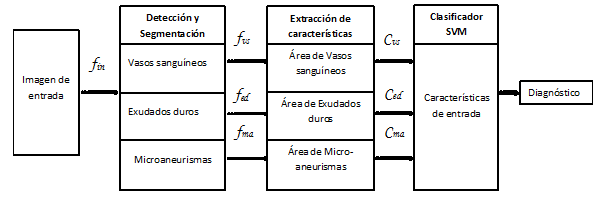
\includegraphics[width=0.6	\textwidth]{./Figures/cap4/metodologiaa.png}
	\caption{Metodología Propuesta.}
	\label{fig:metodo}
\end{figure}


\section{Módulo 1: Detección y Segmentación}
Como se había mencionado en el capítulo anterior la segmentación es el proceso de asignar una etiqueta  a cada pixel en una imagen, tal que los píxeles con las mismas etiquetas compartan ciertas características visuales. El objetivo de la segmentación es simplificar y cambiar la representación de una imagen en algo que sea más significativo y fácil de analizar \cite{seg1,seg2}.
  
La segmentación de imágenes es usada par localizar estructuras y patologías de los ojos tales como vasos sanguíneos, exudados duros y microaneurismas.

\subsection{Detección y segmentación de vasos sanguíneos}


%\subsubsection{Canal verde de la imagen}

Como primer paso en la detección y segmentación de vasos sanguíneos se obtiene del canal verde de la imagen de retina $f_{in}$ debido a que la vasos contienen características que aparecen más contrastadas en este canal (FIGURA \ref{fig:vaso_1}). Sobre el canal verde se aplica el estiramiento de contraste utilizando la técnica de ecualización adaptativa del histograma de contraste limitado (CLAHE) \cite{zuiderveld1994contrast} para suavizar el fondo de la imagen (FIGURA \ref{fig:vaso_2}).
\begin{figure}[H]
\centering
\subfigure[Imagen de retina.]{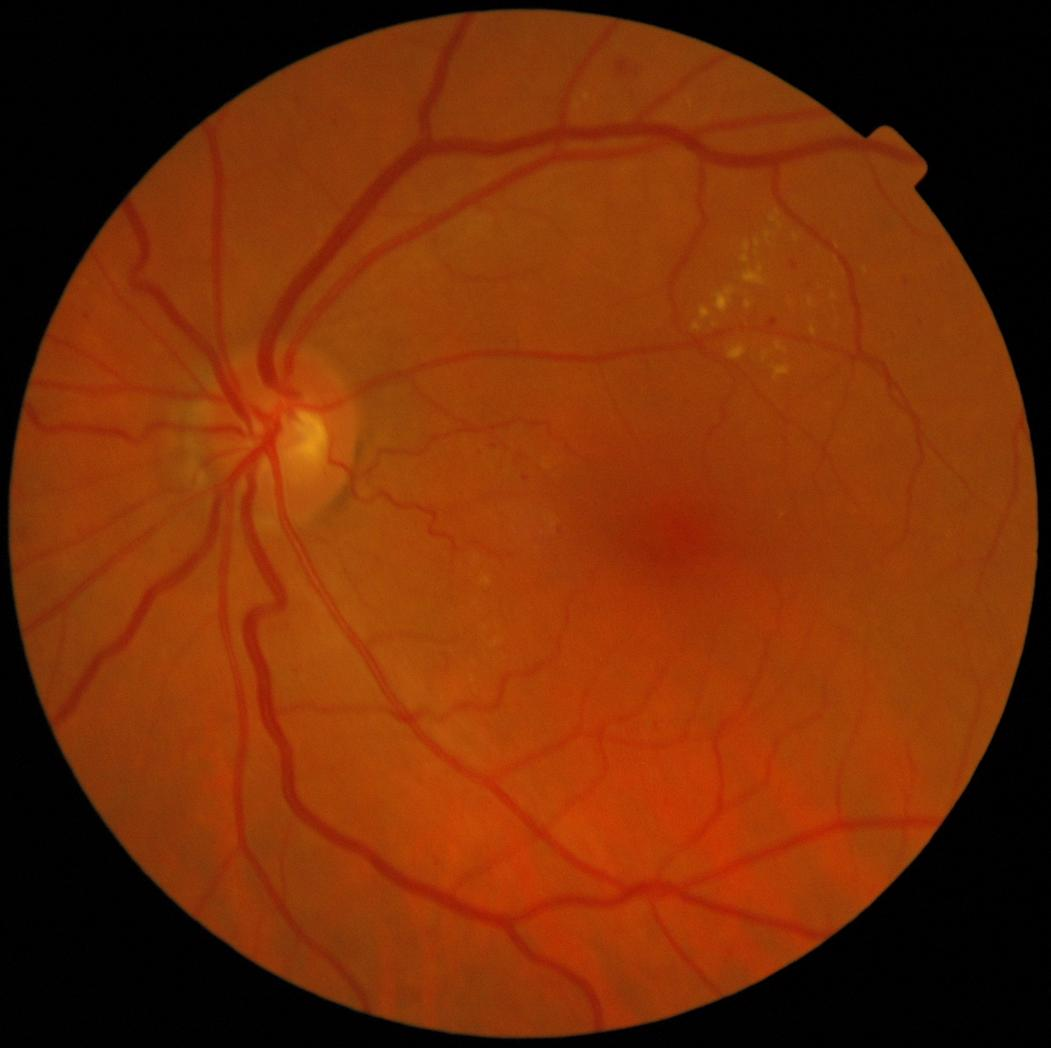
\includegraphics[width=50mm]{./Figures/cap4/vasos/vaso1.jpg}}
\subfigure[Canal verde de la Imagen.]{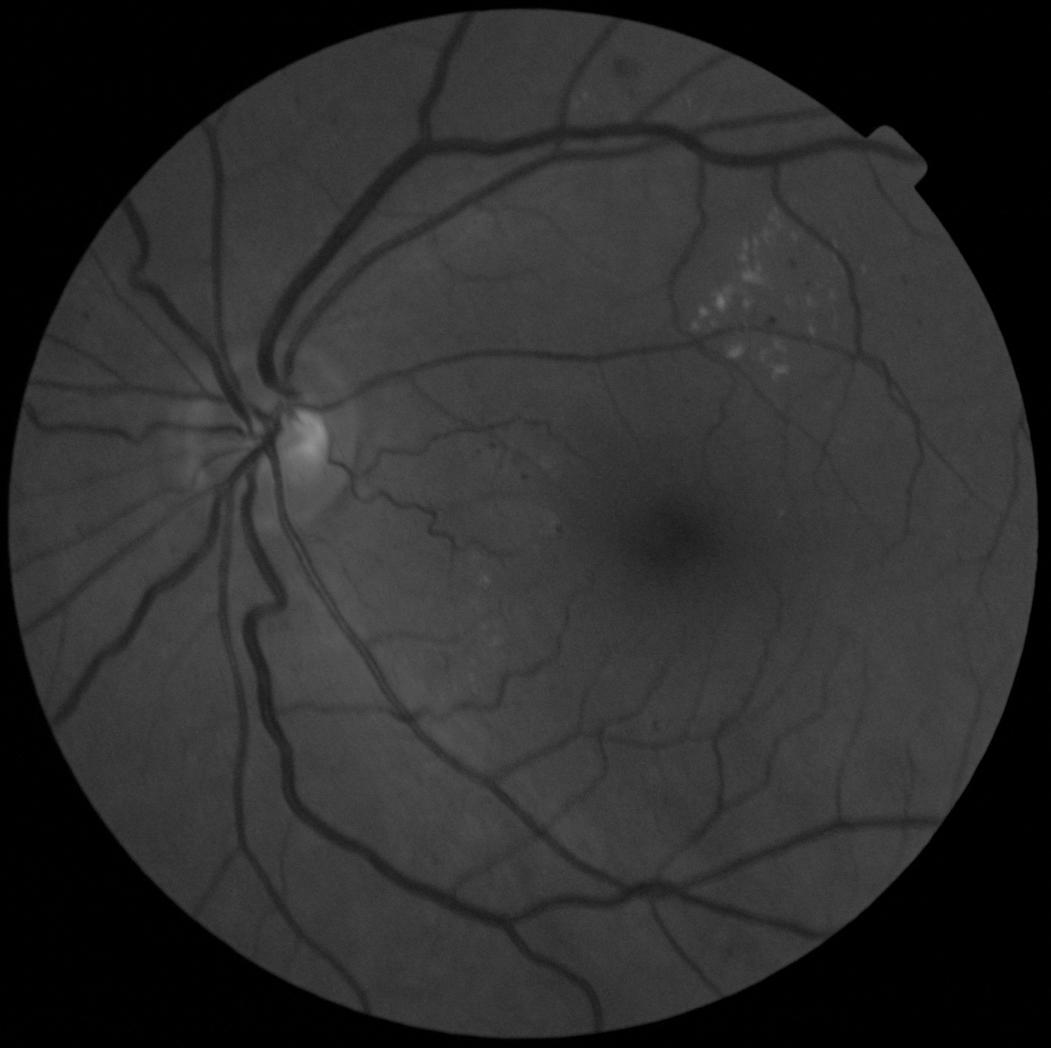
\includegraphics[width=50mm]{./Figures/cap4/micro0.jpg}}
\caption{Canal verde de la imagen.} \label{fig:vaso_1}
\end{figure}

%\subsubsection{CLAHE}

\begin{figure}[H]
\centering
\subfigure[Canal verde de la Imagen.]{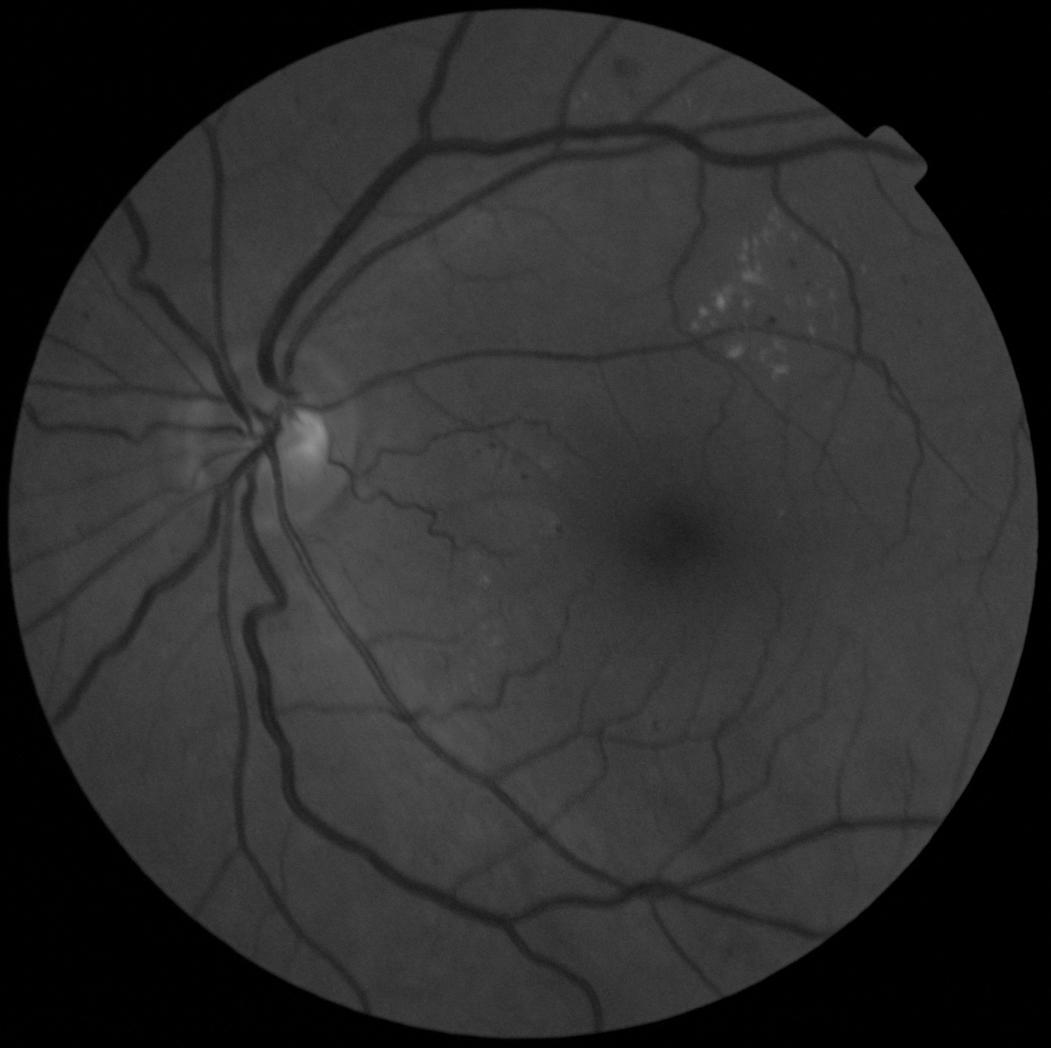
\includegraphics[width=50mm]{./Figures/cap4/micro0.jpg}}
\subfigure[Imagen ecualizada.]{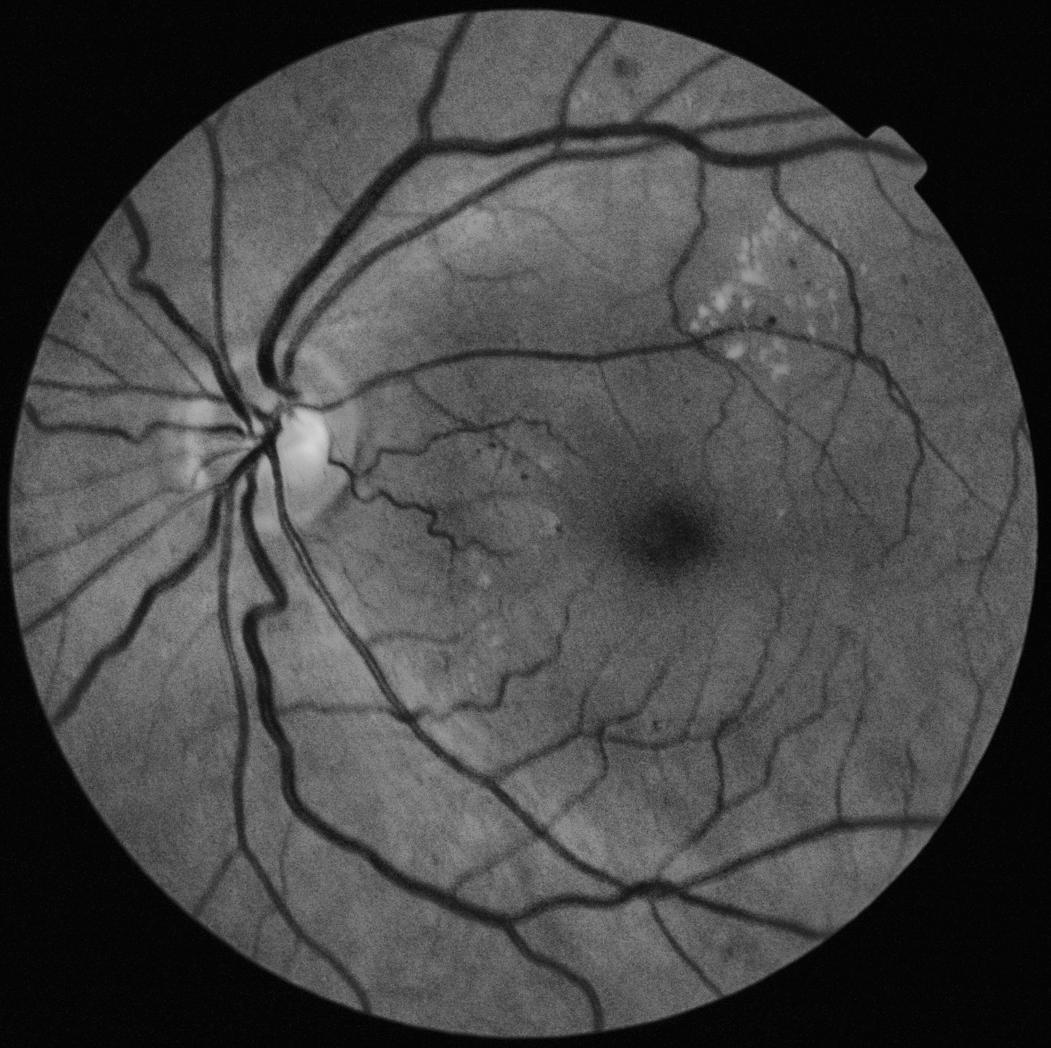
\includegraphics[width=50mm]{./Figures/cap4/vasos/vaso2.jpg}}
\caption{Ecualización del histograma.} \label{fig:vaso_2}
\end{figure}

%\subsubsection{Normalización de la intensidad}
Luego se normaliza la intensidad de tal manera que la misma se expanda a través del rango de intensidad obteniendo la imagen normalizada (FIGURA \ref{fig:vaso_3}). Sobre esta imagen se aplica el filtro de la mediana para obtener una imagen de fondo (FIGURA \ref{fig:vaso_4}).
 
\begin{figure}[H]
\centering
\subfigure[Imagen ecualizada.]{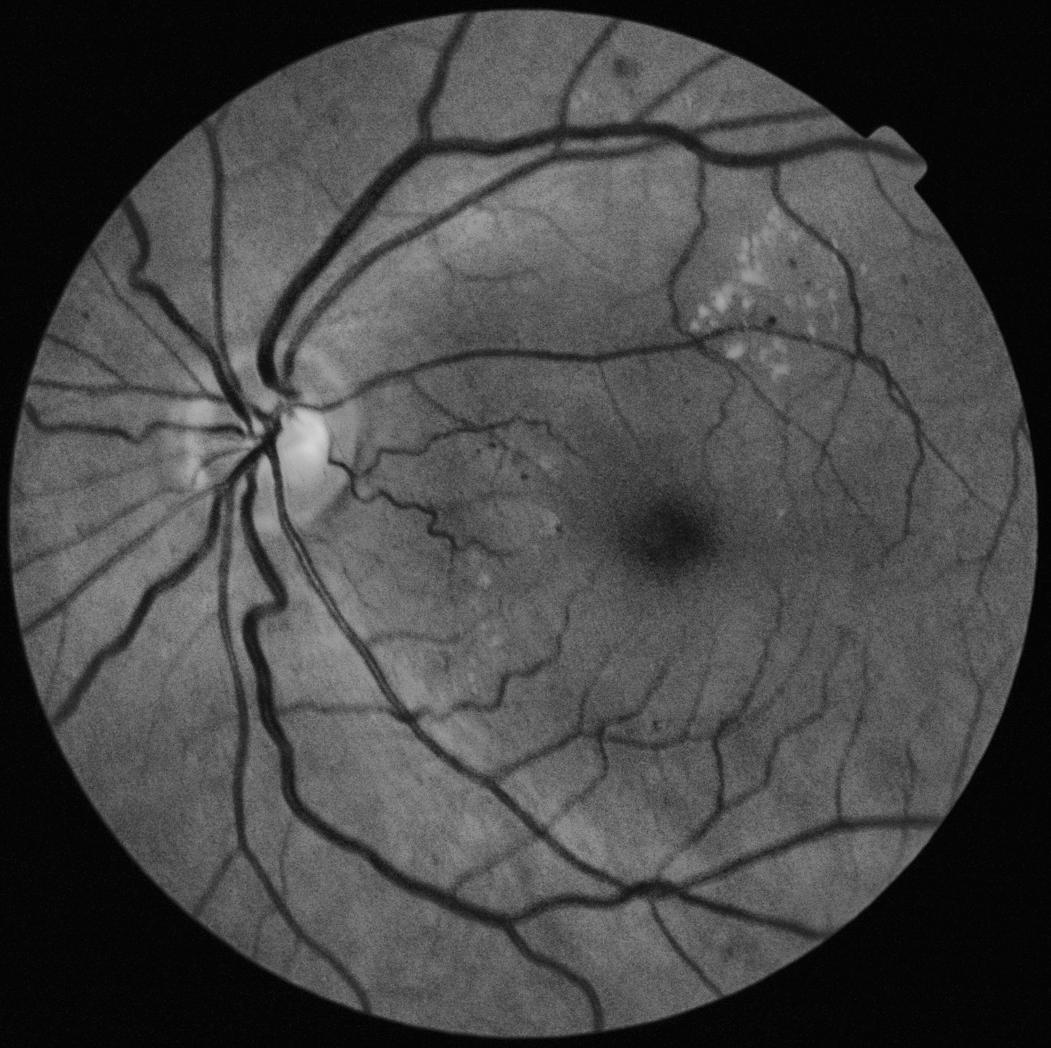
\includegraphics[width=50mm]{./Figures/cap4/vasos/vaso2.jpg}}
\subfigure[Imagen normalizada.]{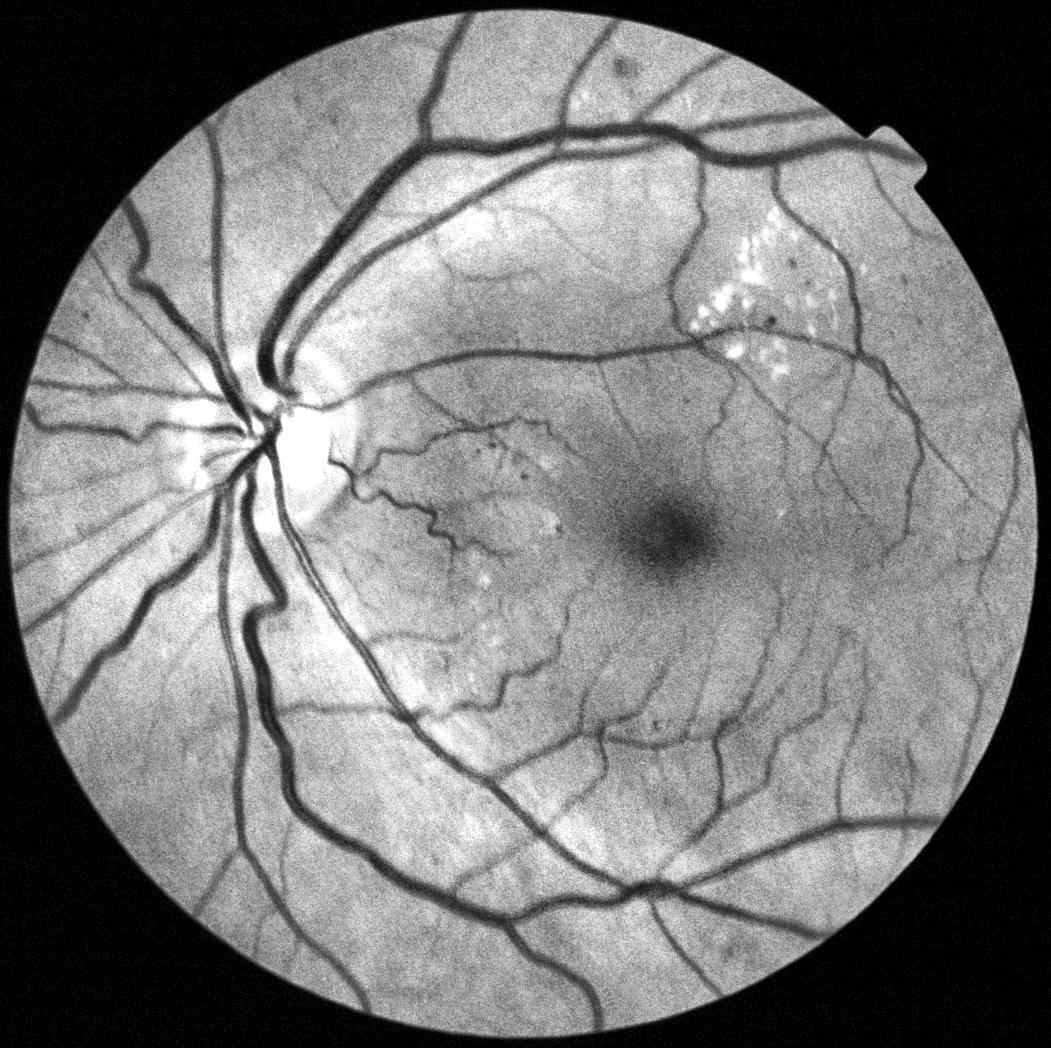
\includegraphics[width=50mm]{./Figures/cap4/vasos/vaso3.jpg}}
\caption{Normalización de la intensidad.} \label{fig:vaso_3}
\end{figure}


%\subsubsection{Filtro de la mediana}

\begin{figure}[H]
\centering
\subfigure[Imagen normalizada.]{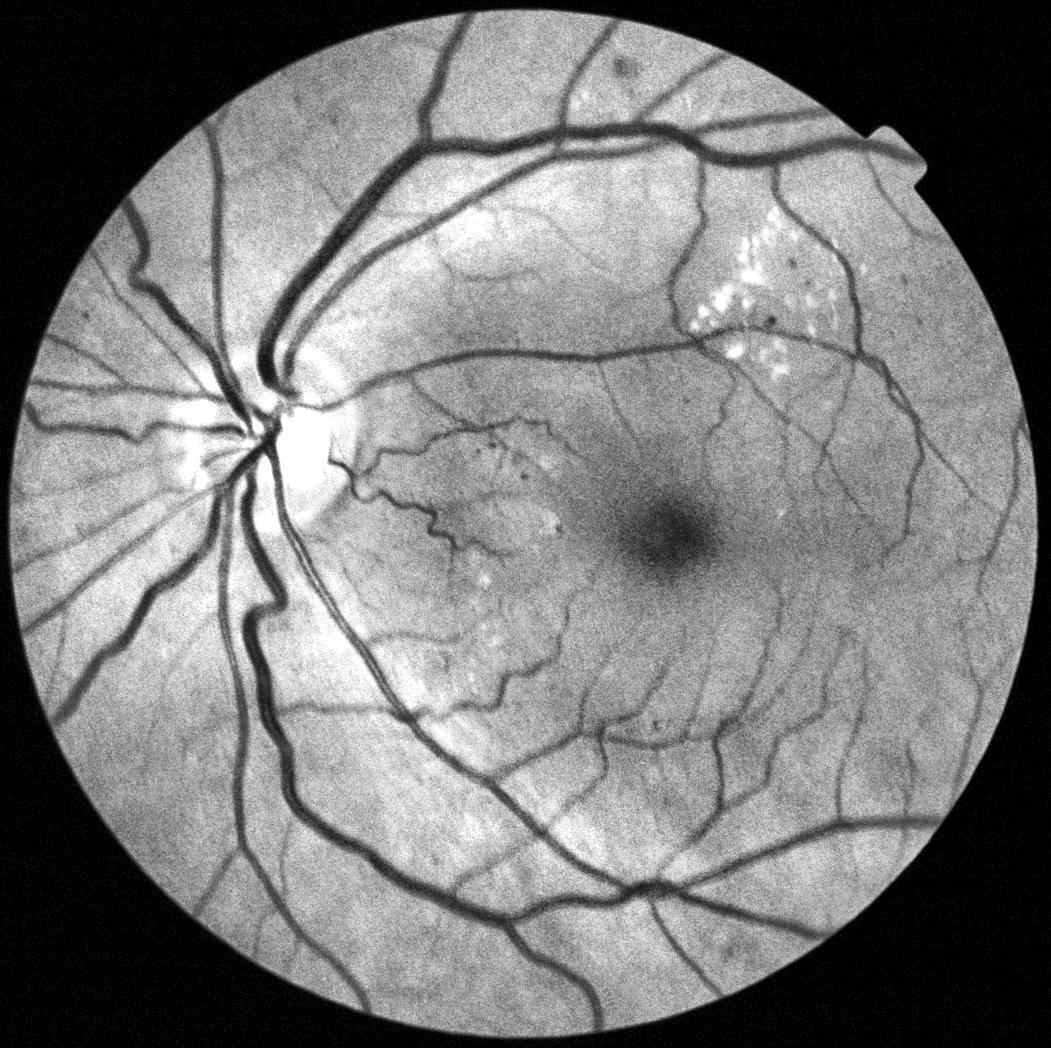
\includegraphics[width=50mm]{./Figures/cap4/vasos/vaso3.jpg}}
\subfigure[Imagen filtrada.]{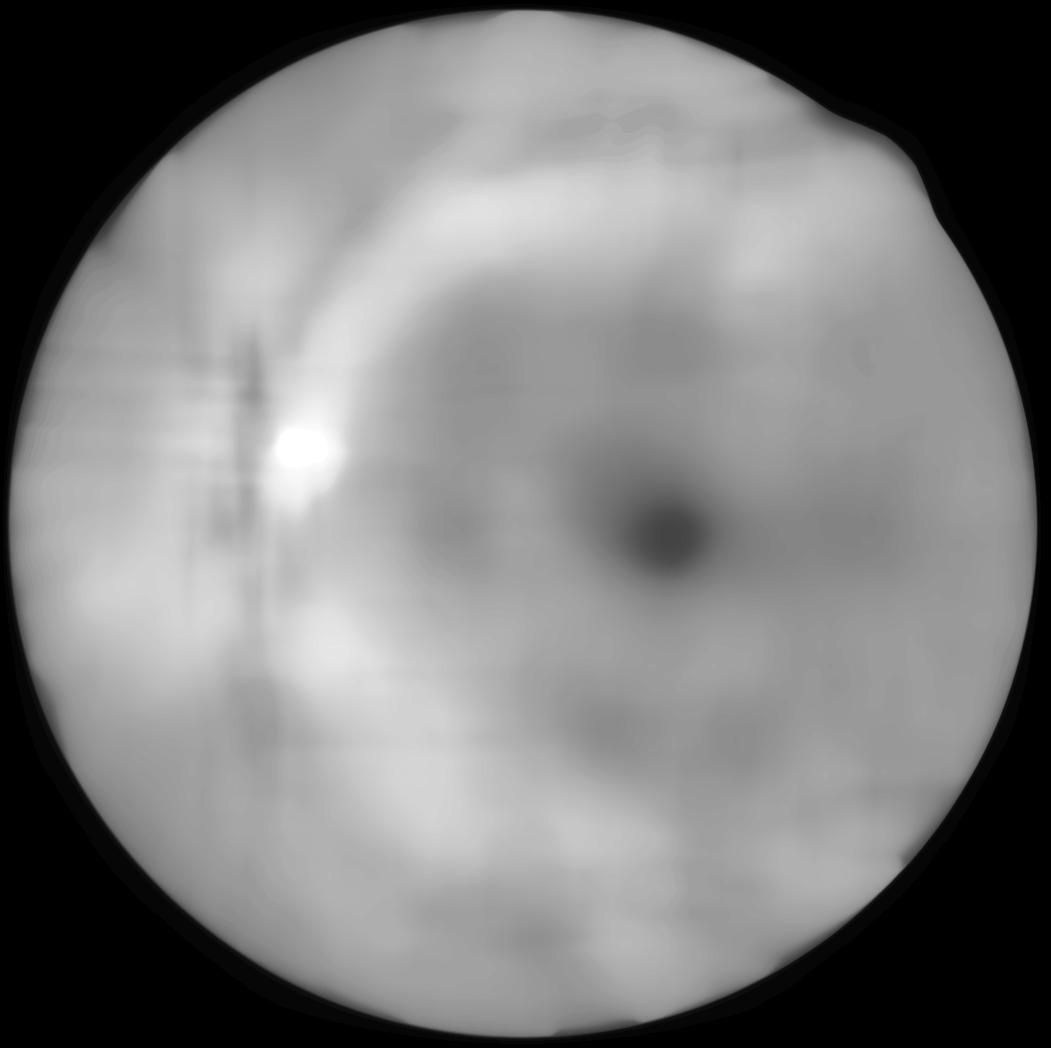
\includegraphics[width=50mm]{./Figures/cap4/vasos/vaso4.jpg}}
\caption{Filtro de la mediana.} \label{fig:vaso_4}
\end{figure}

%\subsubsection{Resta de imágenes}

%\subsubsection{Umbralización}
 Se resta de la imágen de fondo la imagen normalizada dando como resultado una imagen con vasos resaltados (FIGURA \ref{fig:vaso_5}). Esta imagen es umbralizada y se obtienen los vasos sanguíneos en una imagen binaria (FIGURA \ref{fig:vaso_6}).
\begin{figure}[H]
\centering
\subfigure[Imagen filtrada.]{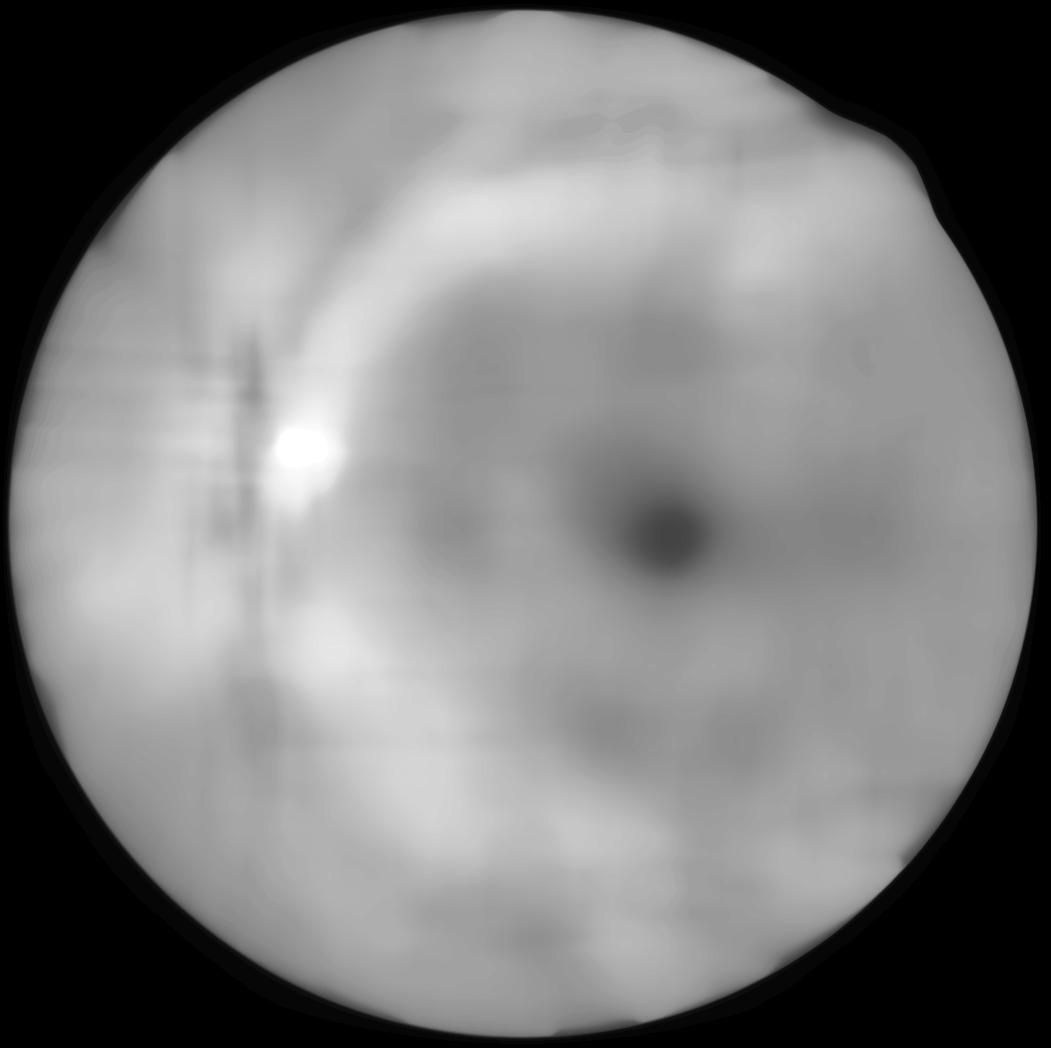
\includegraphics[width=50mm]{./Figures/cap4/vasos/vaso4.jpg}}
\subfigure[Imagen resultante.]{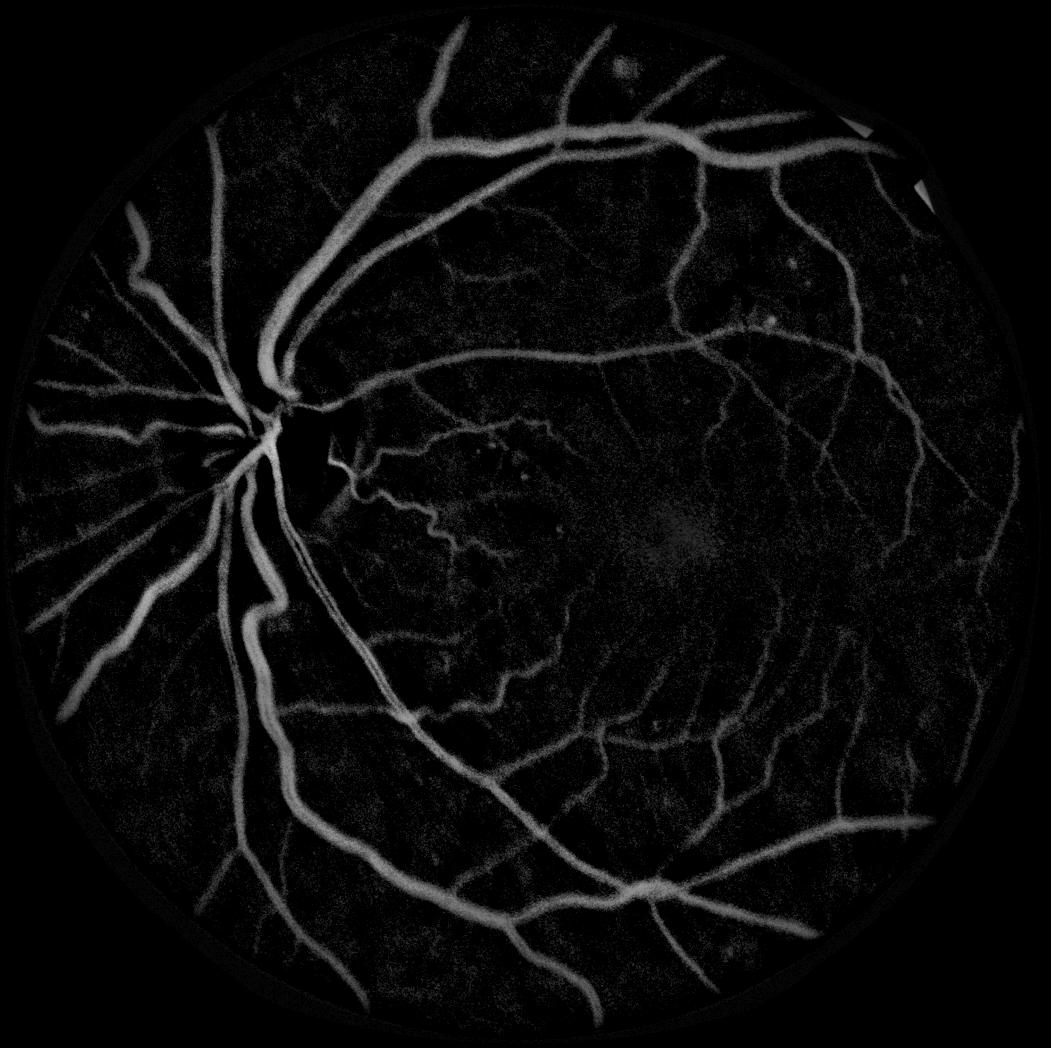
\includegraphics[width=50mm]{./Figures/cap4/vasos/vaso5.jpg}}
\caption{Resta de imágenes.} \label{fig:vaso_5}
\end{figure}


 
\begin{figure}[H]
\centering
\subfigure[Imagen resultante.]{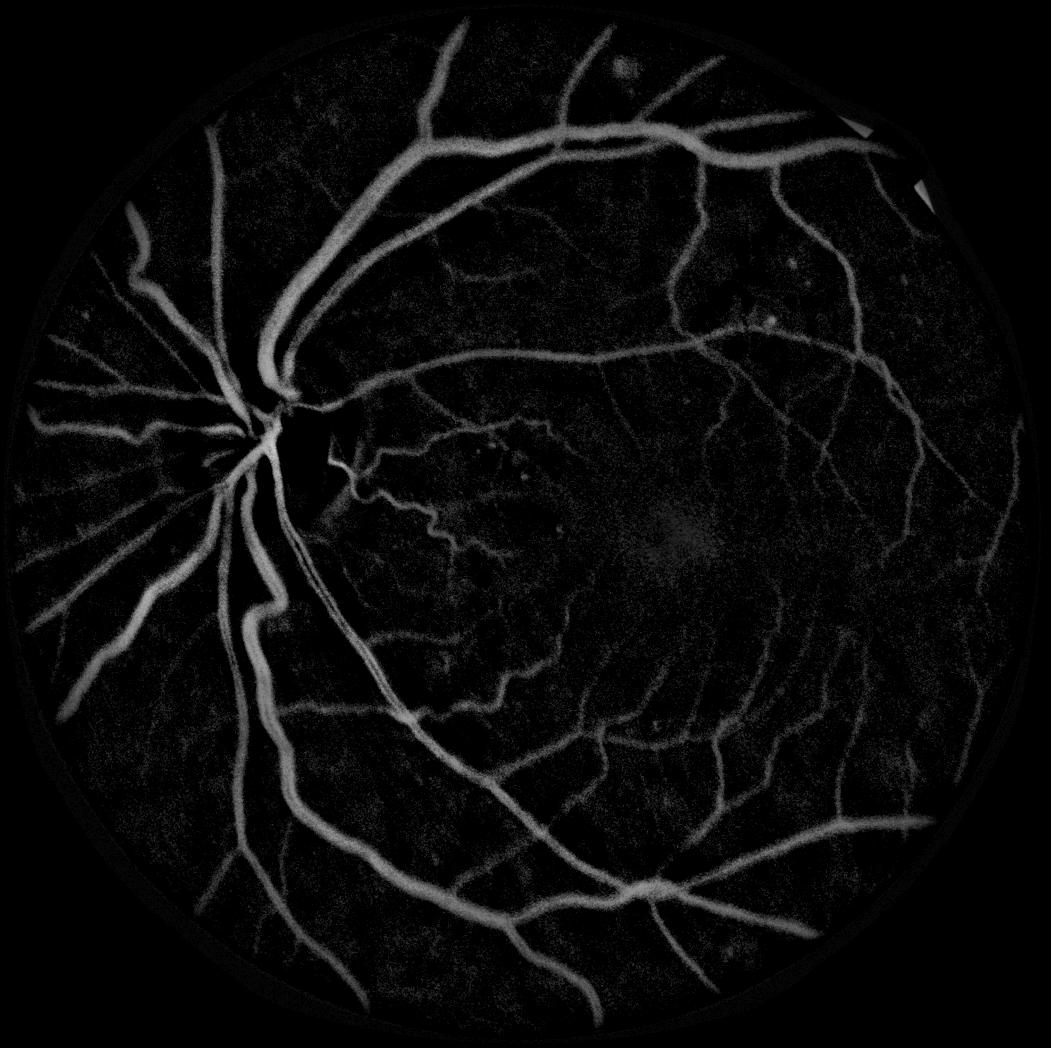
\includegraphics[width=50mm]{./Figures/cap4/vasos/vaso5.jpg}}
\subfigure[Imagen umbralizada.]{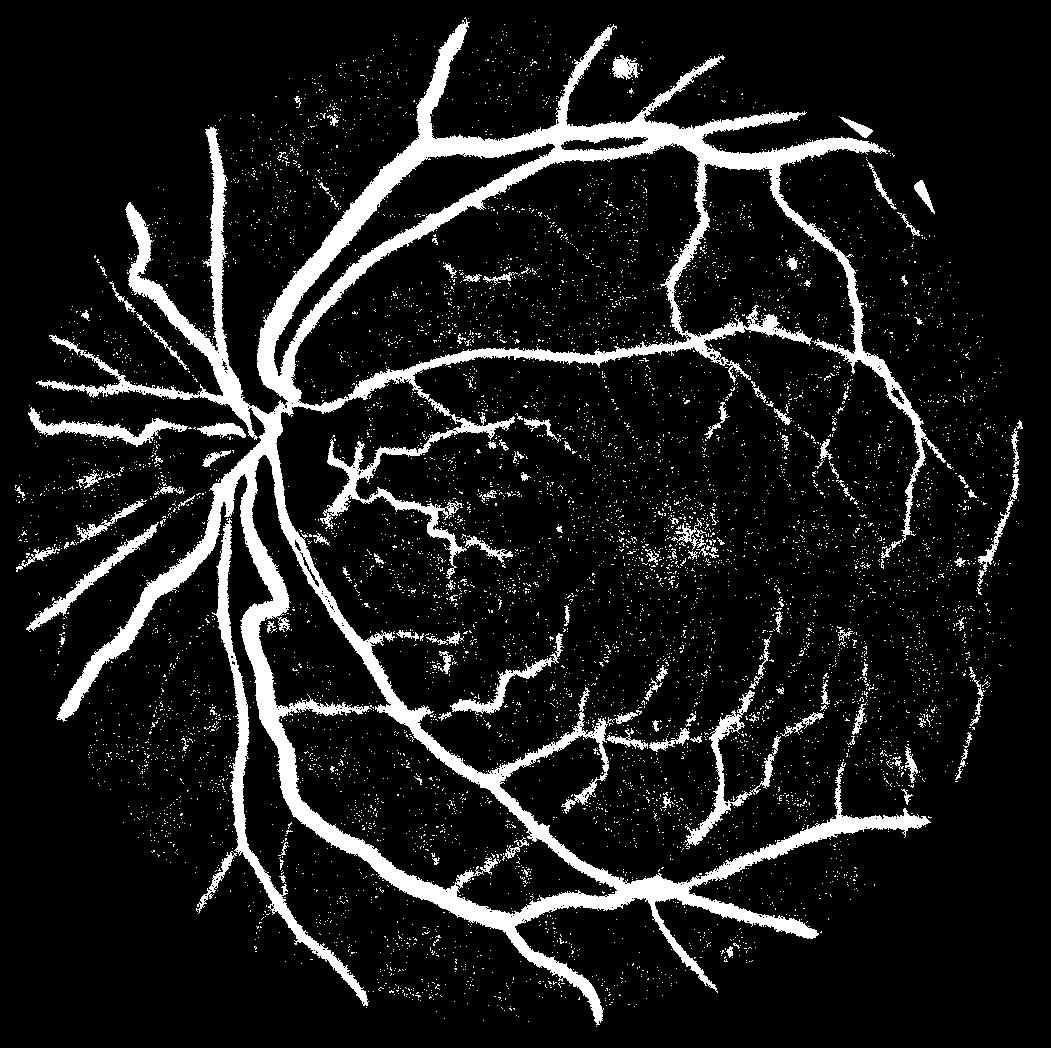
\includegraphics[width=50mm]{./Figures/cap4/vasos/vaso6.jpg}}
\caption{Umbralización.} \label{fig:vaso_6}
\end{figure}

%\subsubsection{Cierre de una imagen}
Luego, se aplica un cierre con elemento estructurante con forma de línea con un tamaño de 7 píxeles de manera a acentuar los vasos (FIGURA \ref{fig:vaso_7}). Para remover el ruido contenido en la imagen binaria se elimina los componentes conectados pequeños resultando en la imagen final $f_{vs}$ (FIGURA \ref{fig:vaso_8}). 

\begin{figure}[H]
\centering
\subfigure[Imagen umbralizada.]{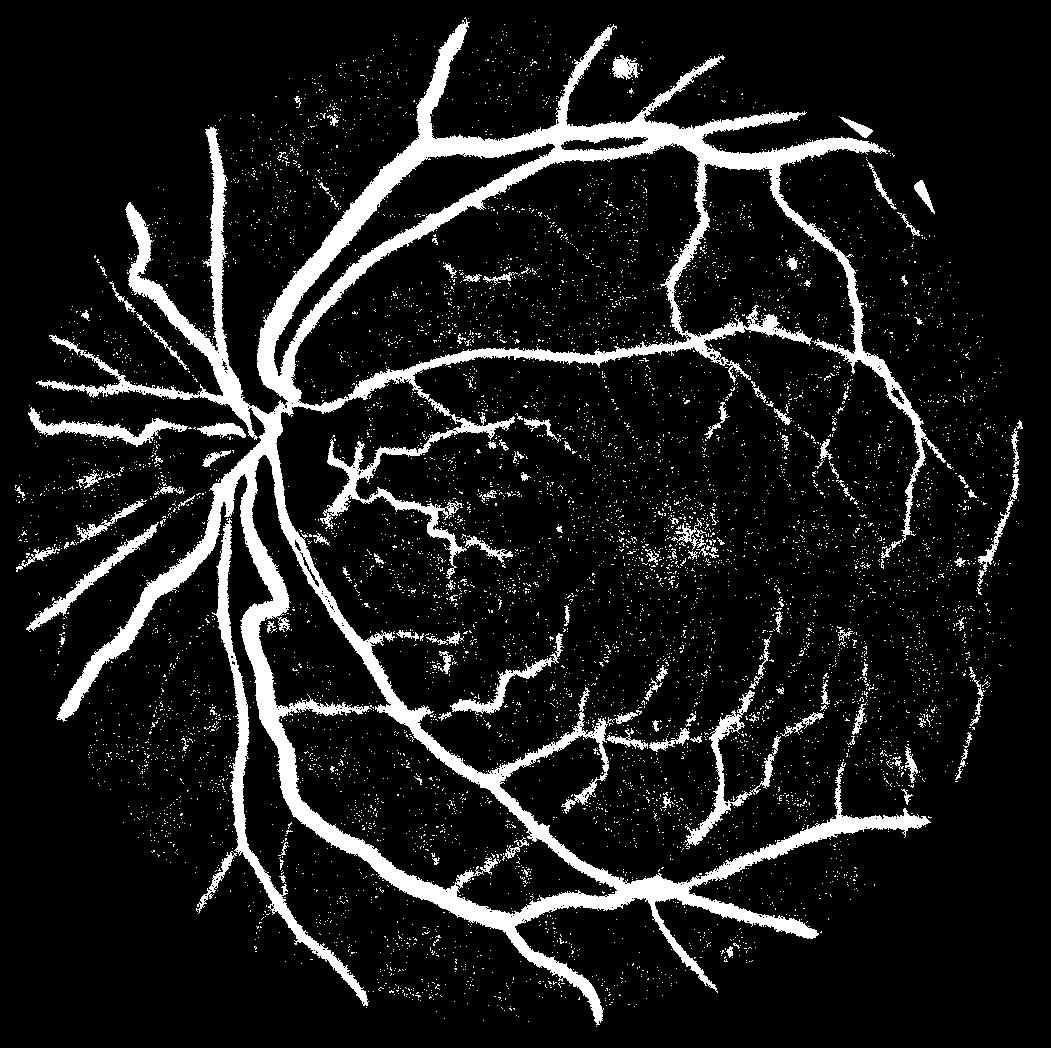
\includegraphics[width=50mm]{./Figures/cap4/vasos/vaso6.jpg}}
\subfigure[Cierre de  imagen.]{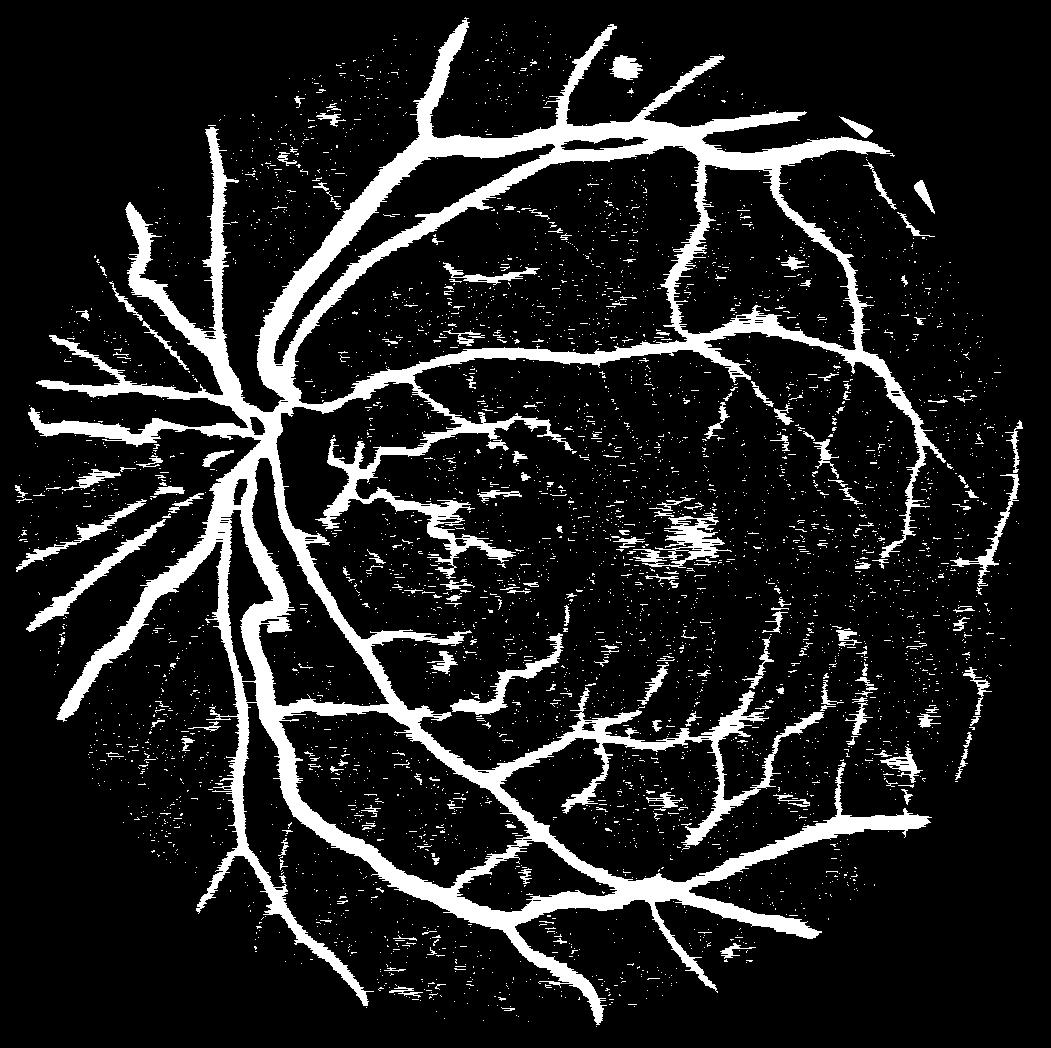
\includegraphics[width=50mm]{./Figures/cap4/vasos/vaso7.jpg}}
\caption{Cierre de una imagen.} \label{fig:vaso_7}
\end{figure}

%\subsubsection{Eliminar componentes conectados pequeños}

\begin{figure}[H]
\centering
\subfigure[Cierre de imagen]{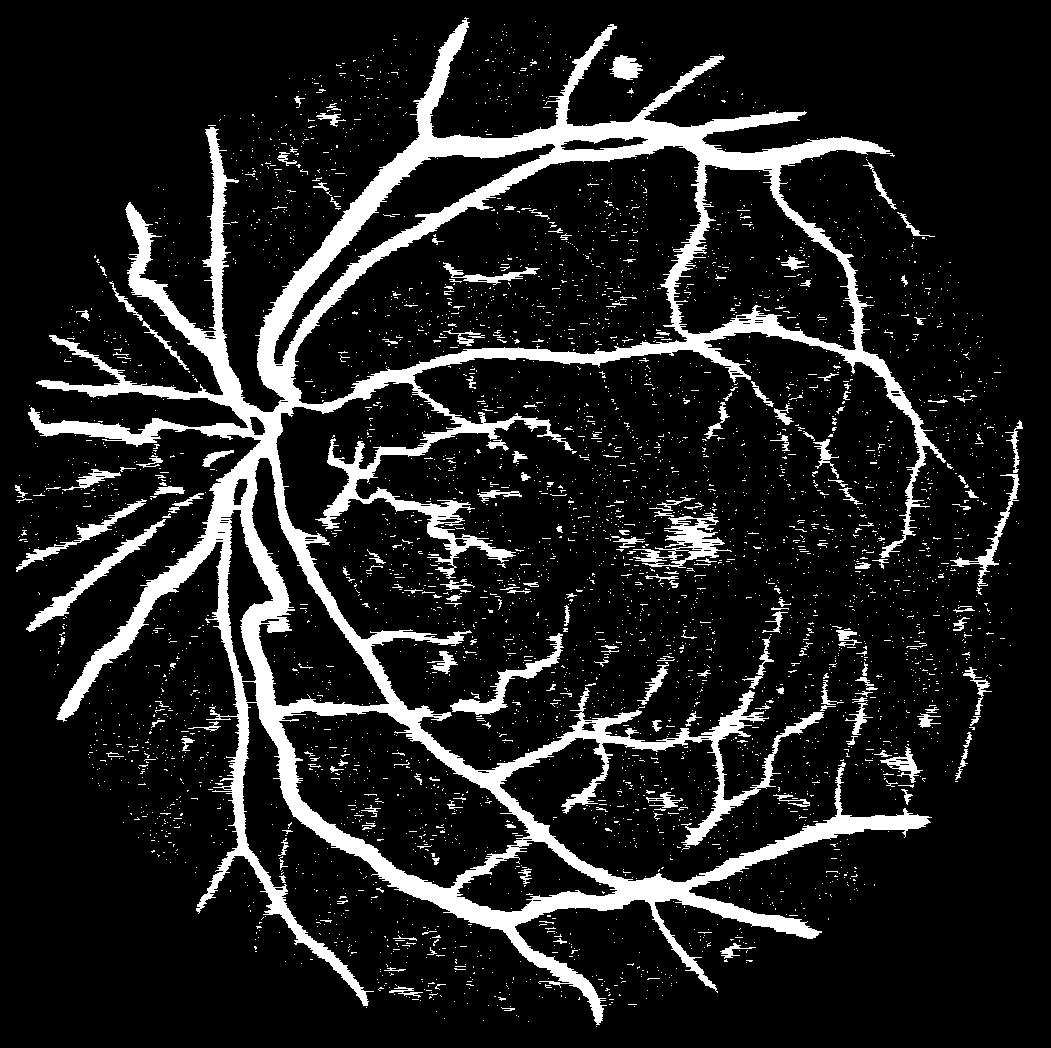
\includegraphics[width=50mm]{./Figures/cap4/vasos/vaso8.jpg}}
\subfigure[Imagen final de vasos sanguíneos.]{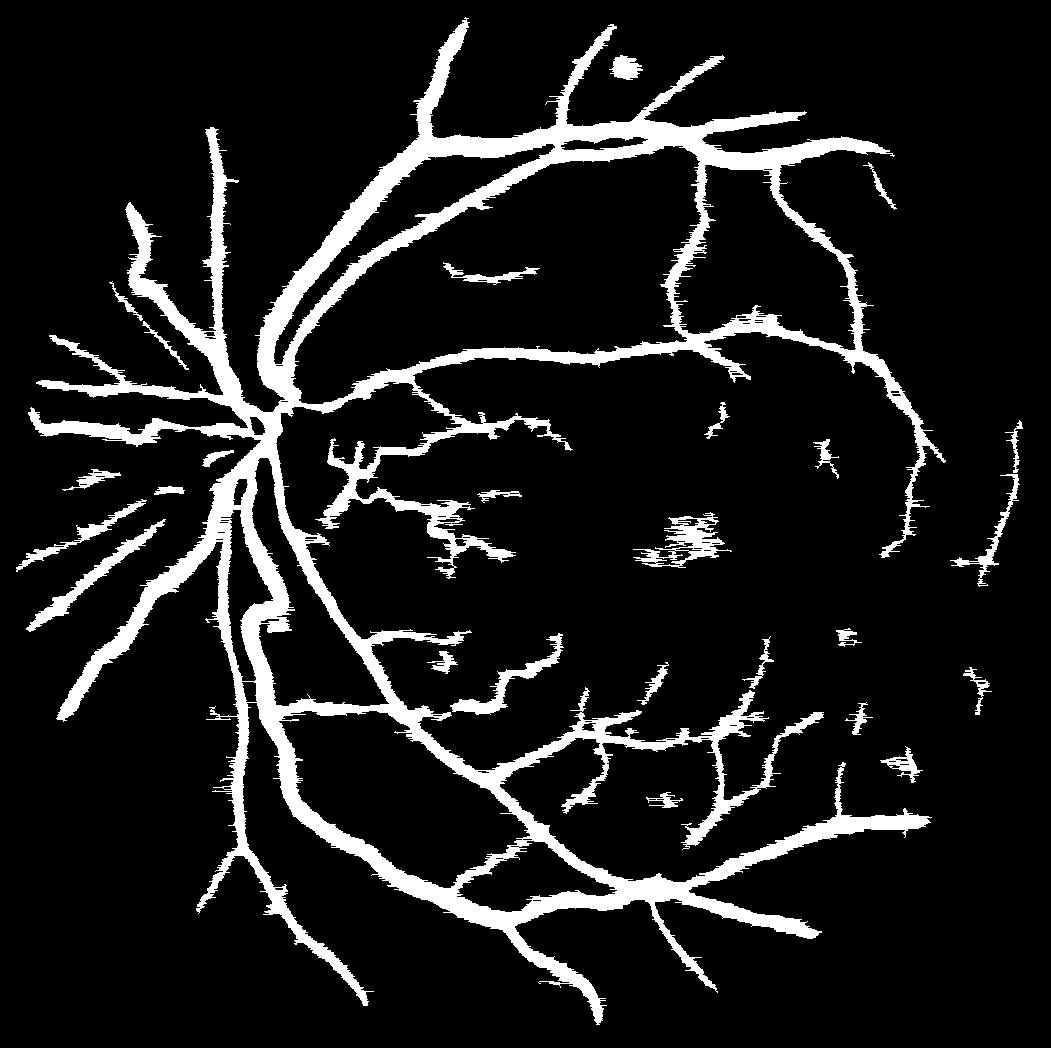
\includegraphics[width=50mm]{./Figures/cap4/vasos/vaso9.jpg}}
\caption{Imagen final $f_{vs}$.} \label{fig:vaso_8}
\end{figure}

La secuencia de pasos para la detección y segmentación de vasos sanguíneos puede verse en la FIGURA \ref{fig:bloquesVS}.
%y la secuencia de imágenes generadas son desplegadas en la FIGURA \ref{fig:secVena}.




\begin{figure}[H]
	\centering
		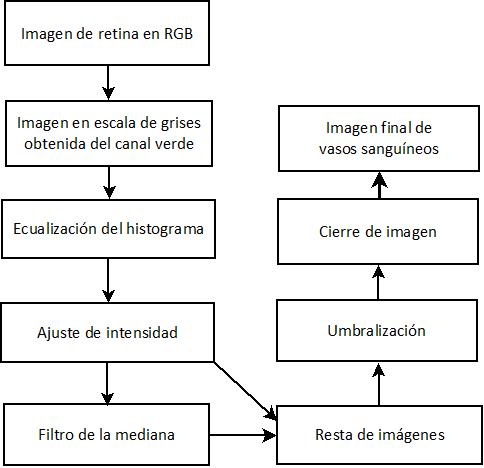
\includegraphics[width=0.7	\textwidth]{./Figures/cap4/dia_vena1.png}
	\caption{Diagrama de bloques de detección y segmentación de vasos sanguíneos.}
	\label{fig:bloquesVS}
\end{figure}

%\begin{figure}[H]
%	\centering
%		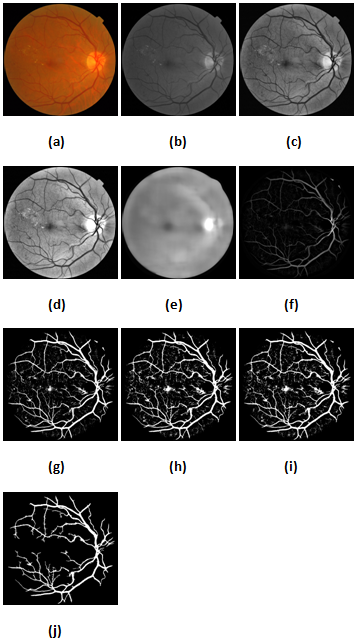
\includegraphics[width=0.7	\textwidth]{./Figures/cap4/sec_vena.png}
%	\caption{Secuencia de imágenes de detección y segmentación de vasos sanguíneos (a) Imagen de retina, (b) Canal verde, (c) Imagen ecualizada, (d) Imagen con intensidad Ajustada, (e) Imagen generada por el filtro de la mediana, (f) Resta de imágenes, (g) Imagen umbralizada, (h) Cierre de la imagen, (i) Imagen sin componentes conectados, (j) Imagen de  vasos sanguíneos segmentada $f_{vs}$.}
%	\label{fig:secVena}
%	\end{figure}
	
%	\subsection{Secuencias de imágenes genradas por el algoritmo de detección de vasos sanguíneos}
	


\subsection{Detección y segmentación de exudados duros} 
La detección y segmentación de los exudados duros necesitan previamente la segmentación y detección del disco óptico y el borde circular. 

\subsubsection{Detección y segmentación de Disco Óptico}
Uno de los mayores problemas a la hora de detectar exudados duros es la similaridad de coloración que los mismos poseen con el disco óptico \cite{el2013automatic}. Para resolver este problema se realiza la detección del disco óptico. 



La imagen original$f_{in}$ en RGB es pasada a escala de grises usando el canal verde de la imagen (FIGURA \ref{fig:disco_1}). Se realiza el estiramiento de contraste utilizando la técnica de ecualización adaptativa del histograma de contraste limitado (CLAHE) para suavizar el fondo de la imagen (FIGURA \ref{fig:disco_2}).

\begin{figure}[H]
\centering
\subfigure[Imagen de retina.]{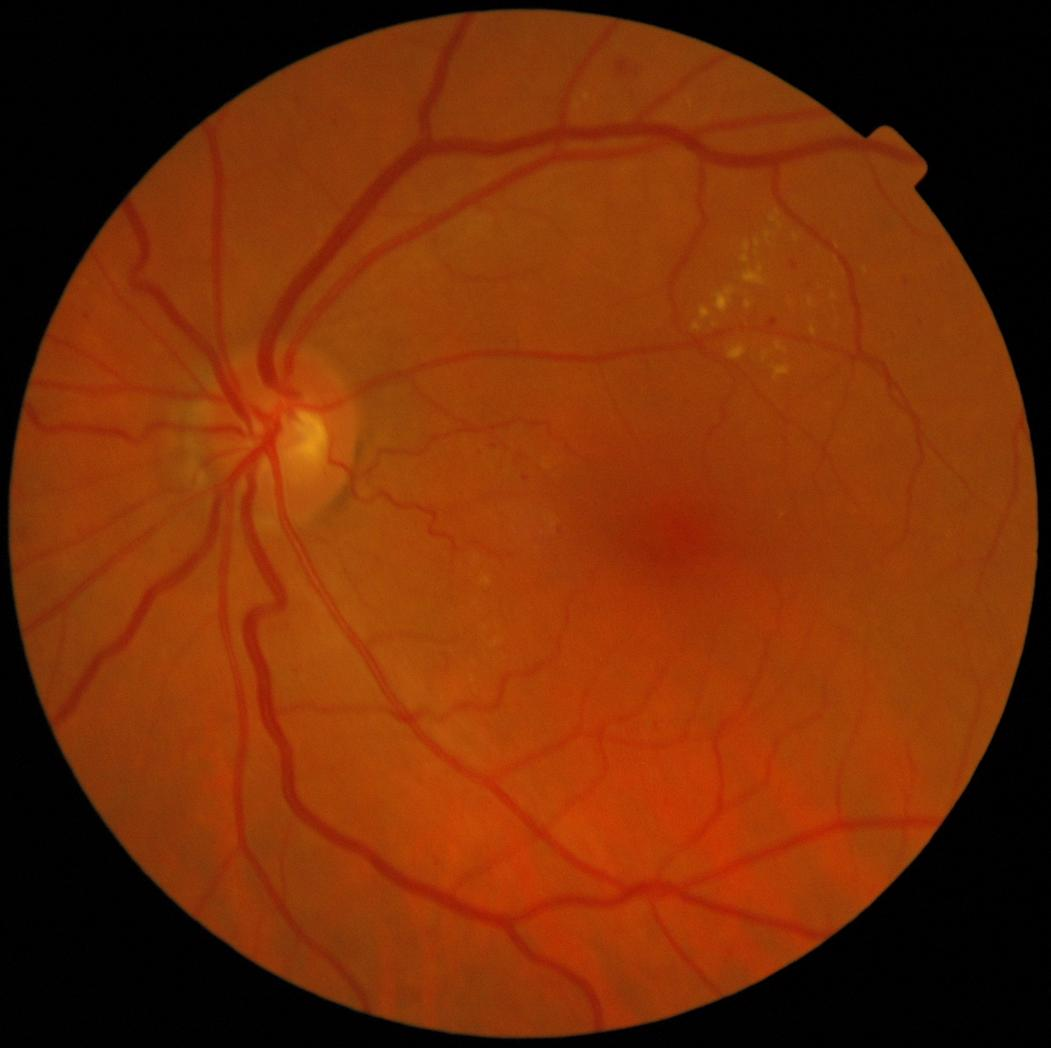
\includegraphics[width=50mm]{./Figures/cap4/vasos/vaso1.jpg}}
\subfigure[Canal verde de la Imagen.]{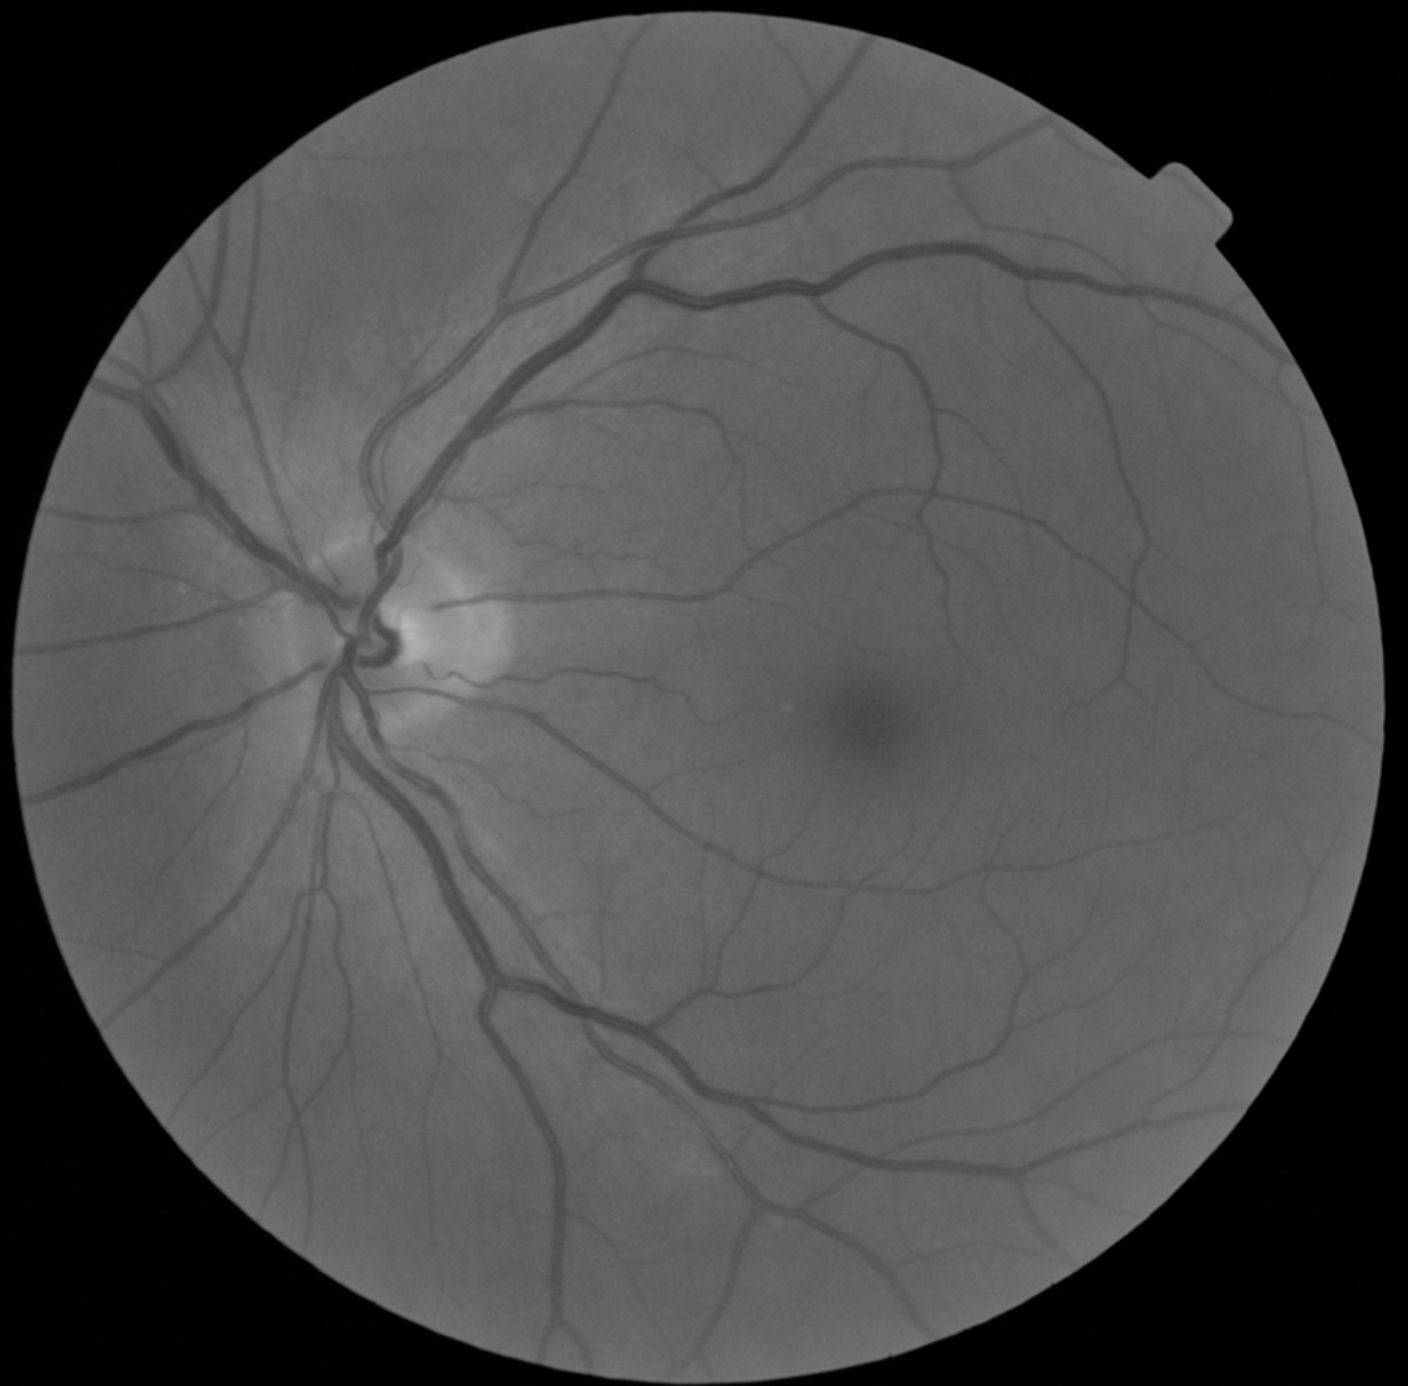
\includegraphics[width=50mm]{./Figures/cap4/disco/disco1.png}}
\caption{Canal verde de la imagen.} \label{fig:disco_1}
\end{figure}

\begin{figure}[H]
\centering
\subfigure[Canal verde de la imagen.]{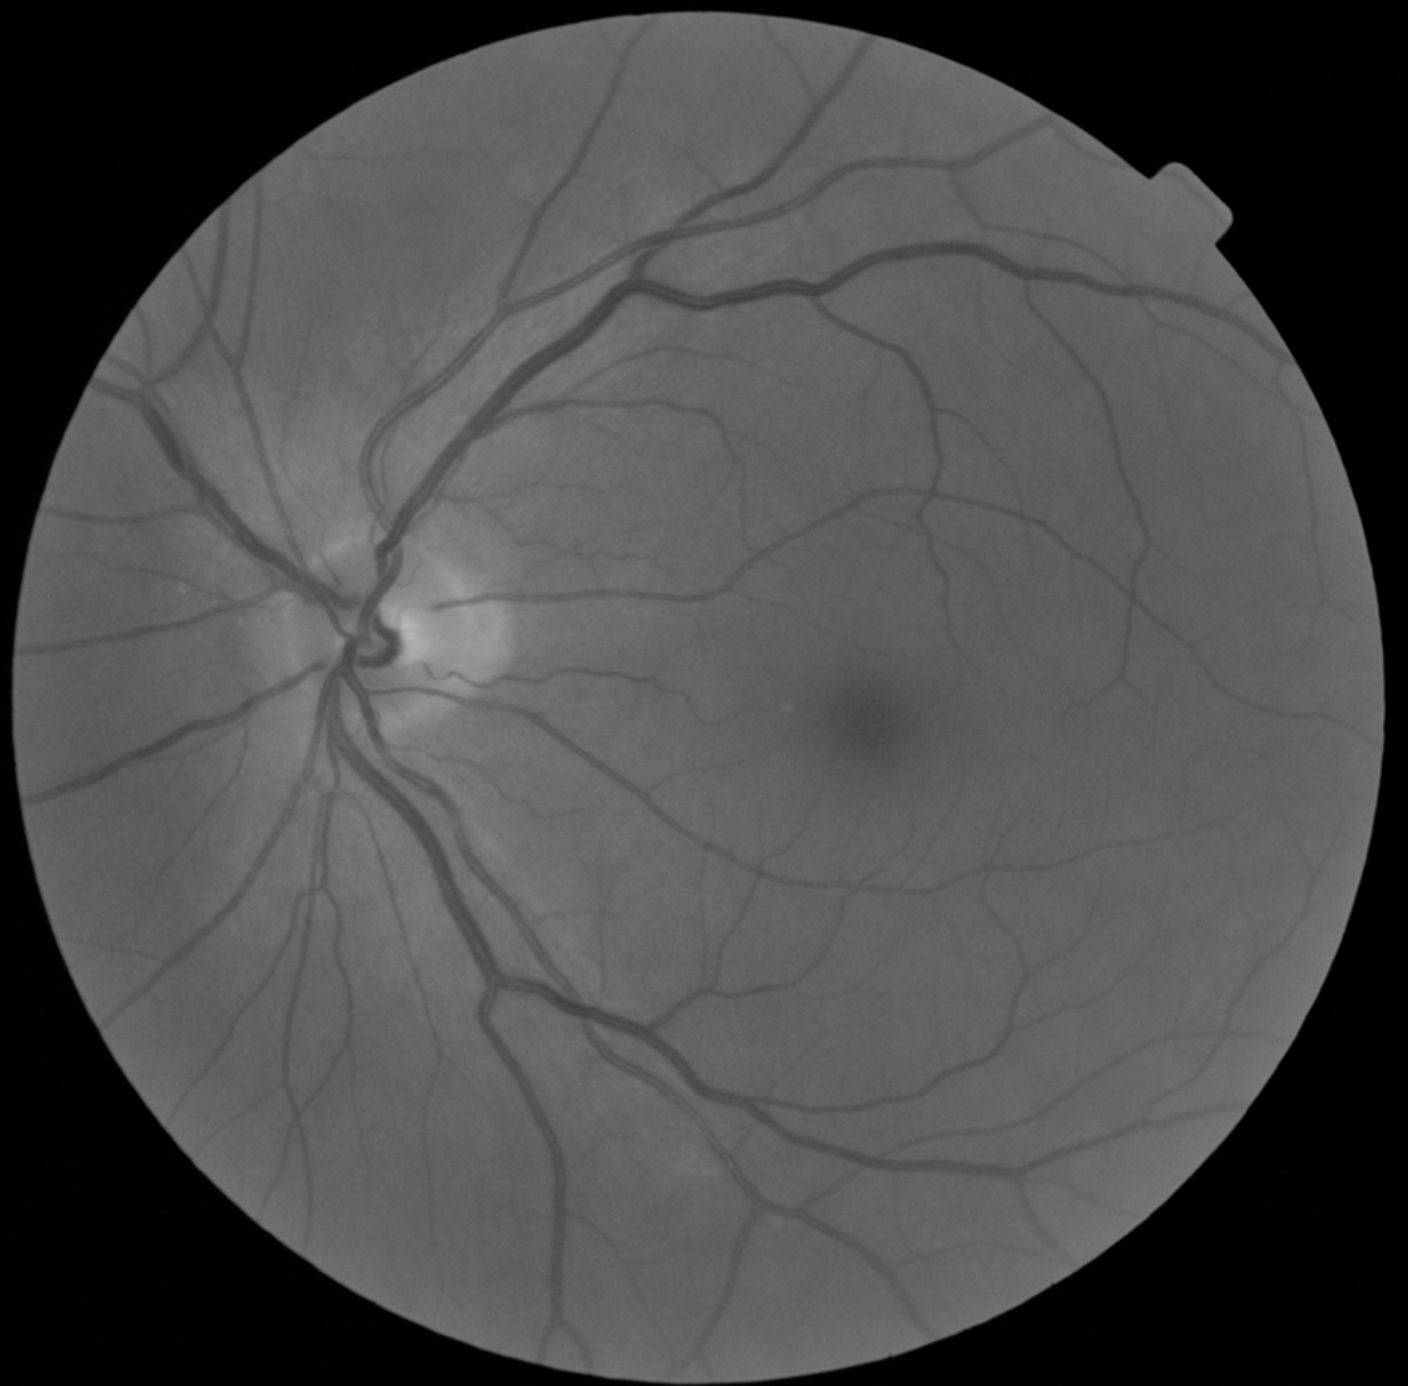
\includegraphics[width=50mm]{./Figures/cap4/disco/disco1.png}}
\subfigure[Imagen ecualizada.]{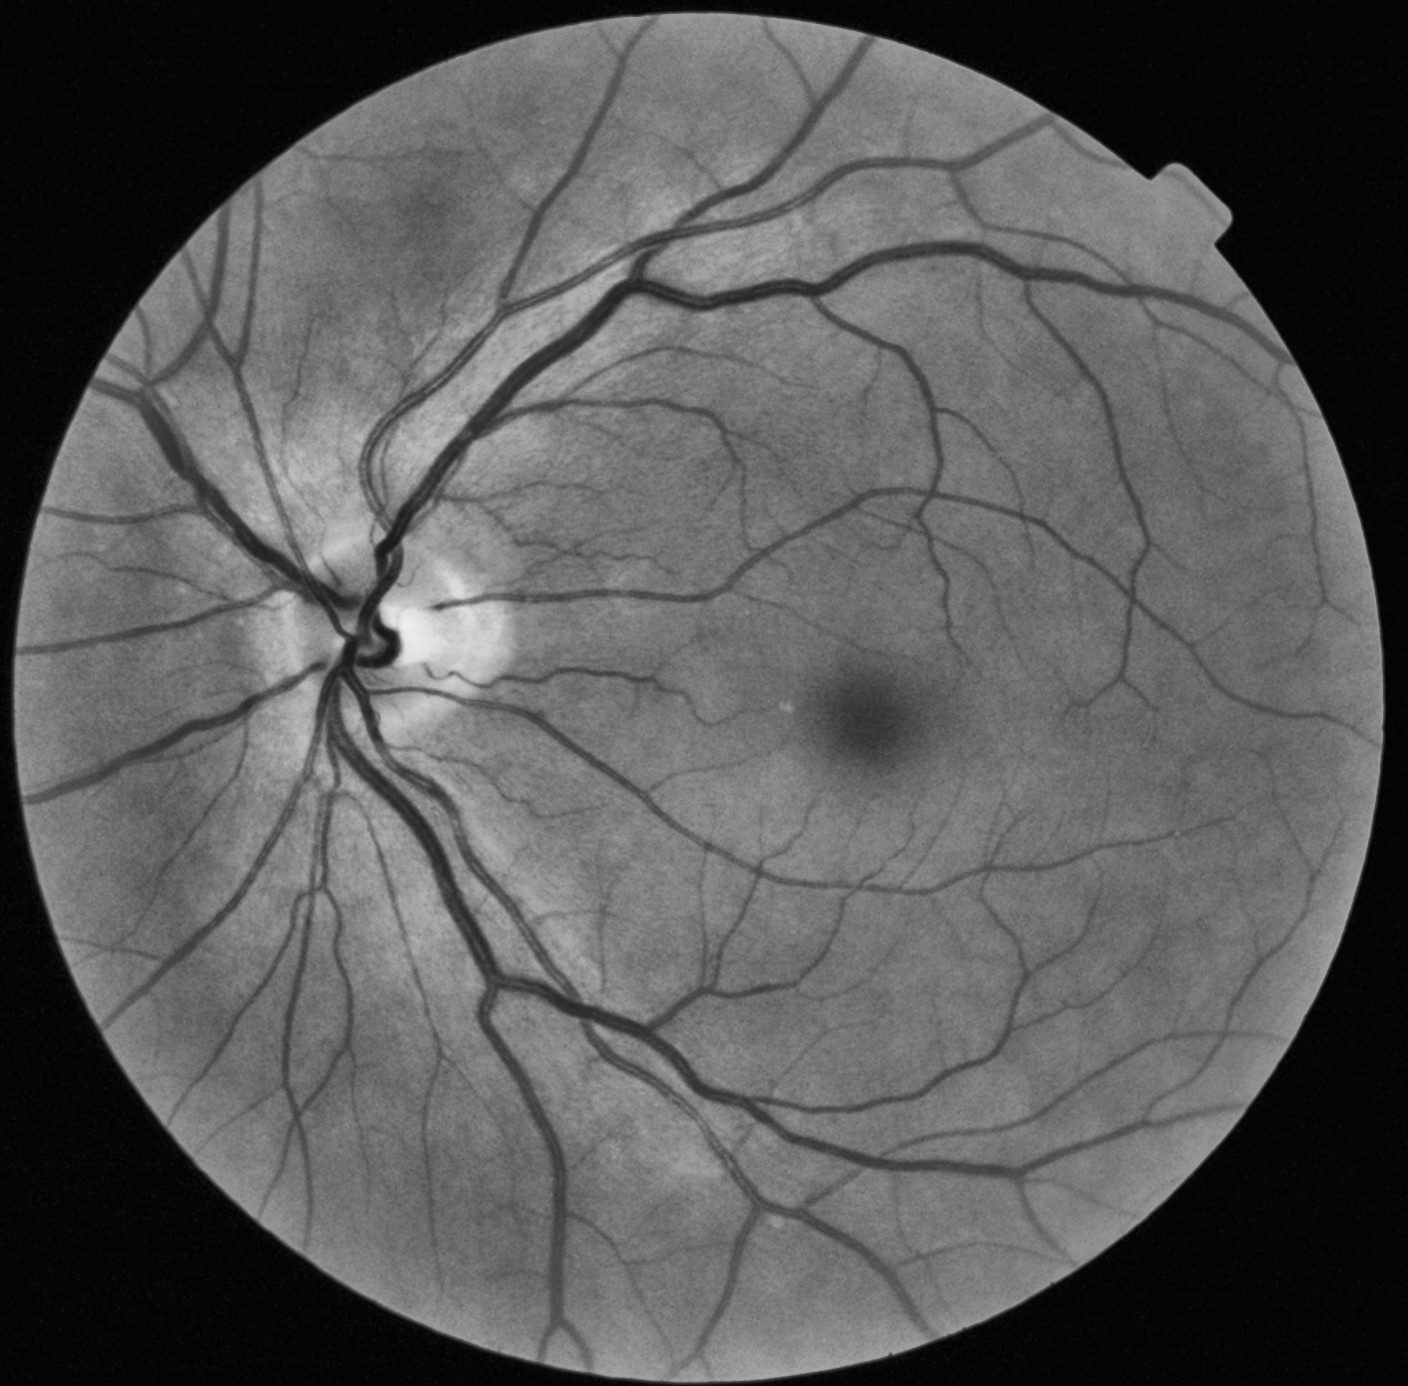
\includegraphics[width=50mm]{./Figures/cap4/disco/disco2.png}}
\caption{Ecualización del histograma.} \label{fig:disco_2}
\end{figure}

Luego  se realiza un ajuste de los valores de intensidad para reducir el ruido de la imagen, de manera a mejorar la imagen ( FIGURA \ref{fig:disco_3}). Como siguiente paso, se procede a la umbralización de la imagen mejorada, obteniendo de esta manera una imagen umbralizada ( FIGURA \ref{fig:disco_4}).

\begin{figure}[H]
\centering
\subfigure[Imagen ecualizada.]{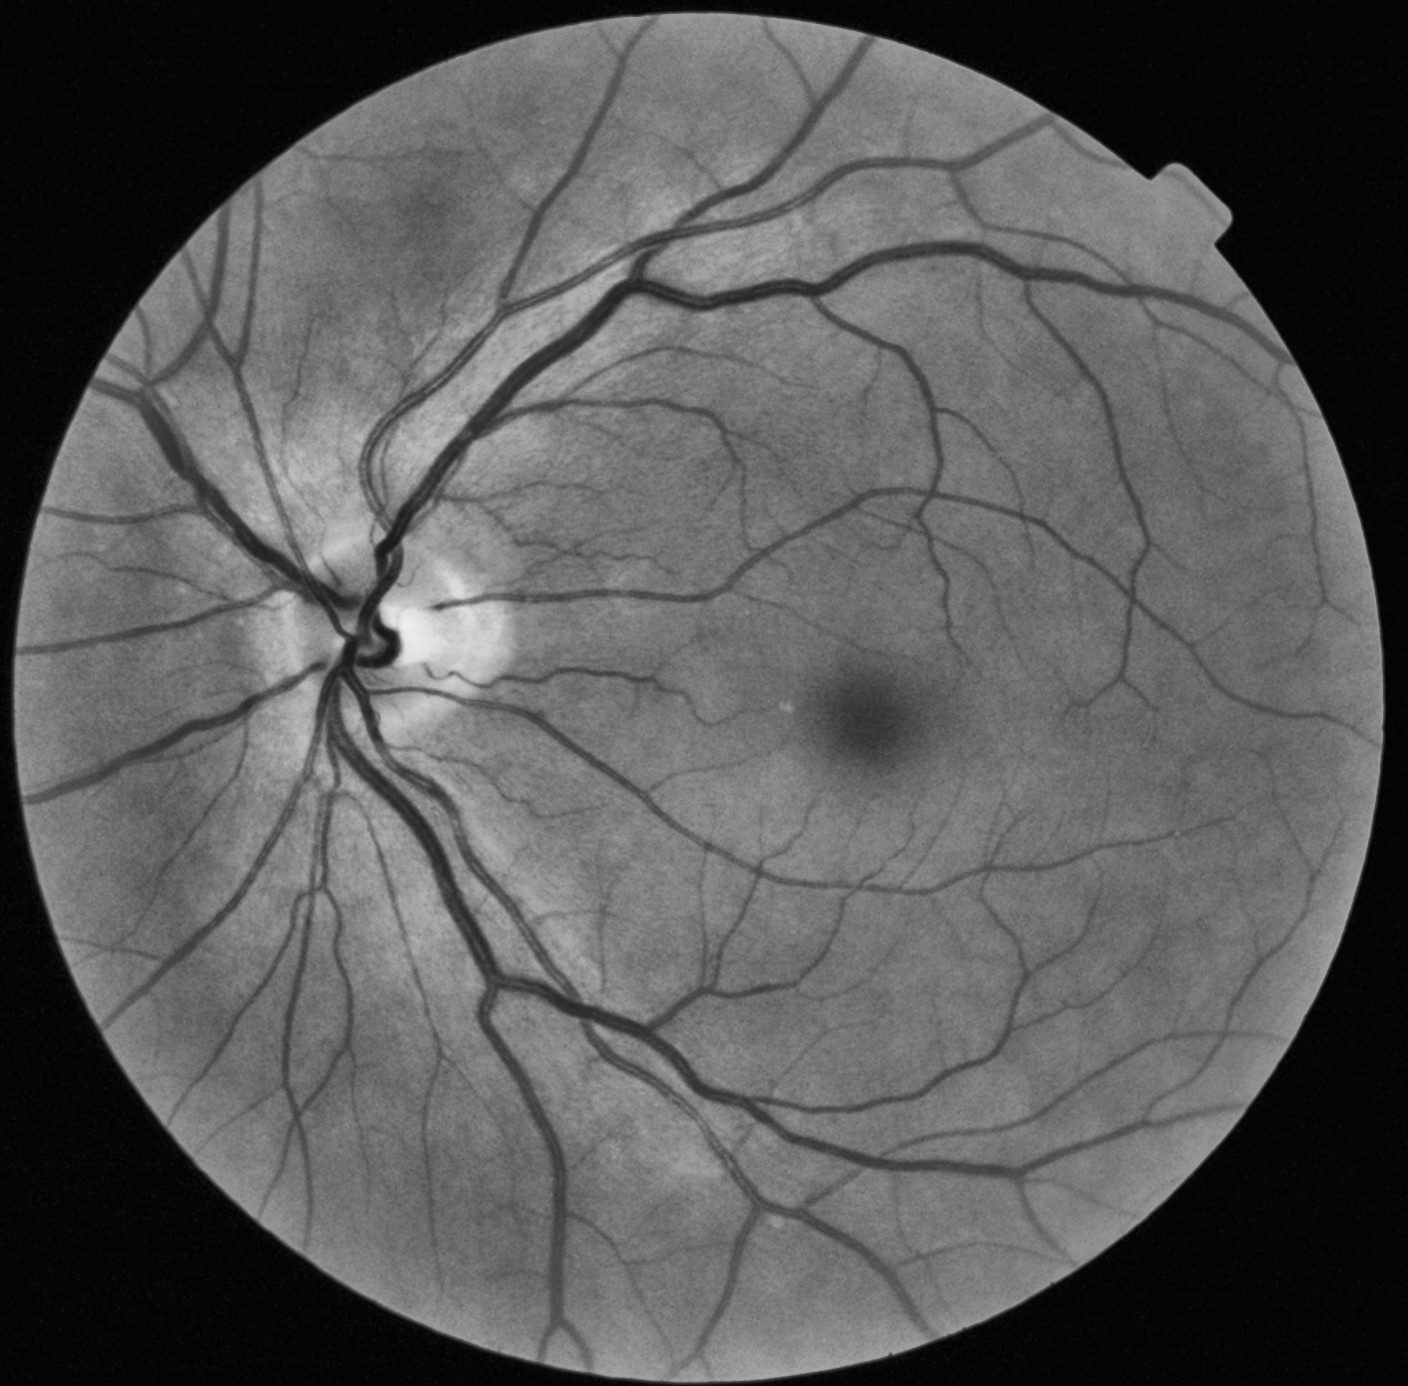
\includegraphics[width=50mm]{./Figures/cap4/disco/disco2.png}}
\subfigure[Imagen con intensidad ajustada.]{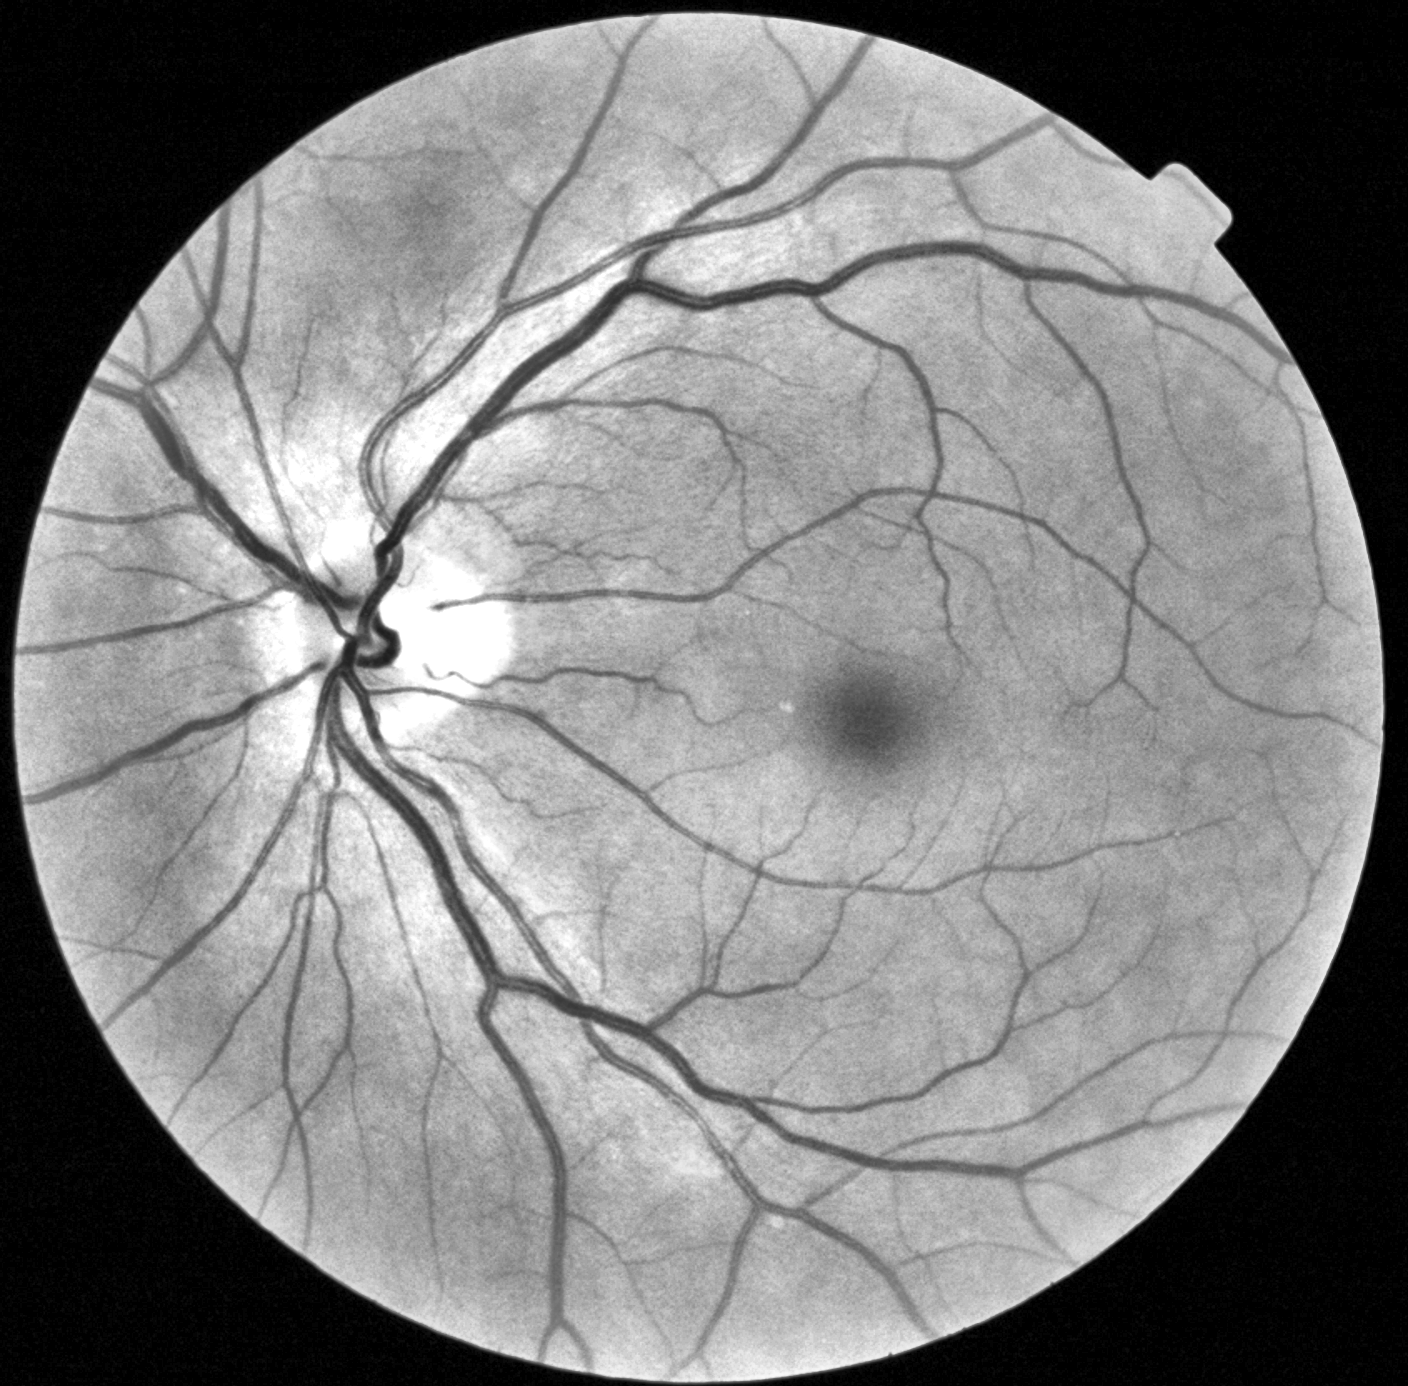
\includegraphics[width=50mm]{./Figures/cap4/disco/disco3.png}}
\caption{Ajuste de intensidad.} \label{fig:disco_3}
\end{figure}

\begin{figure}[H]
\centering
\subfigure[Imagen con intensidad ajustada.]{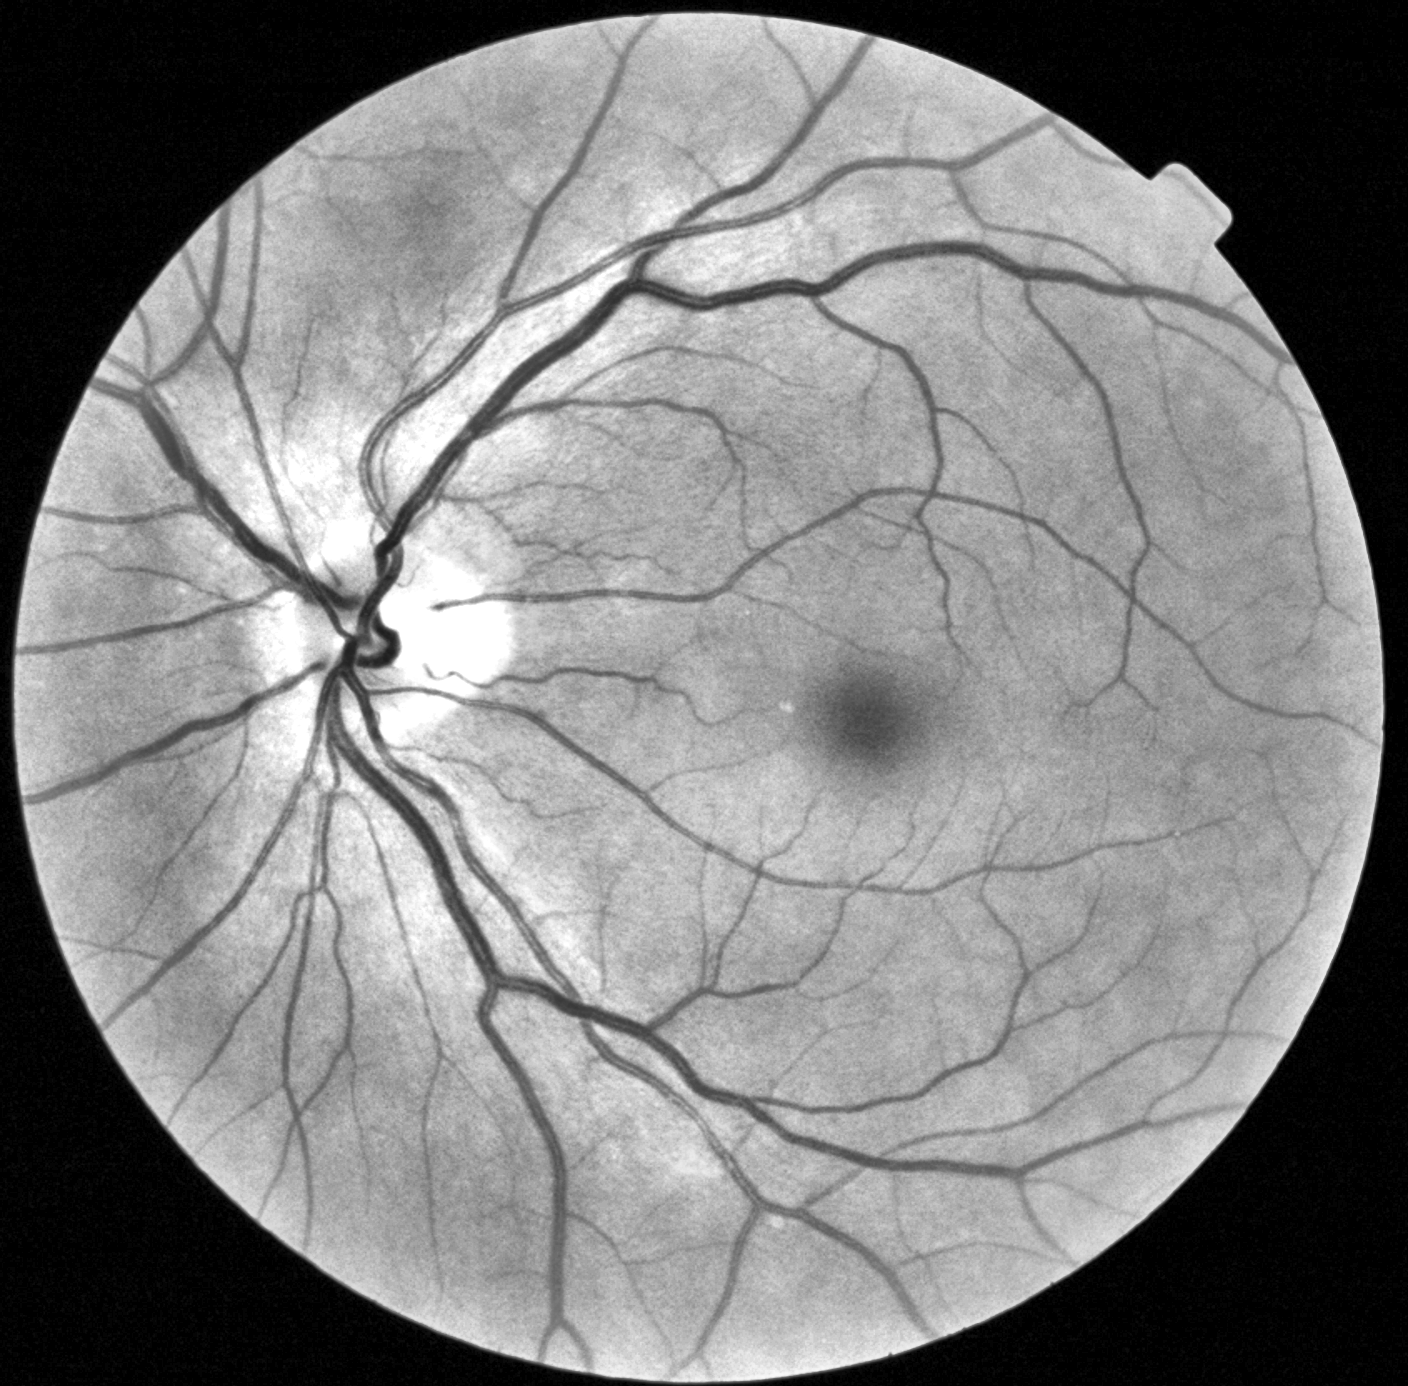
\includegraphics[width=50mm]{./Figures/cap4/disco/disco3.png}}
\subfigure[Imagen umbralizada.]{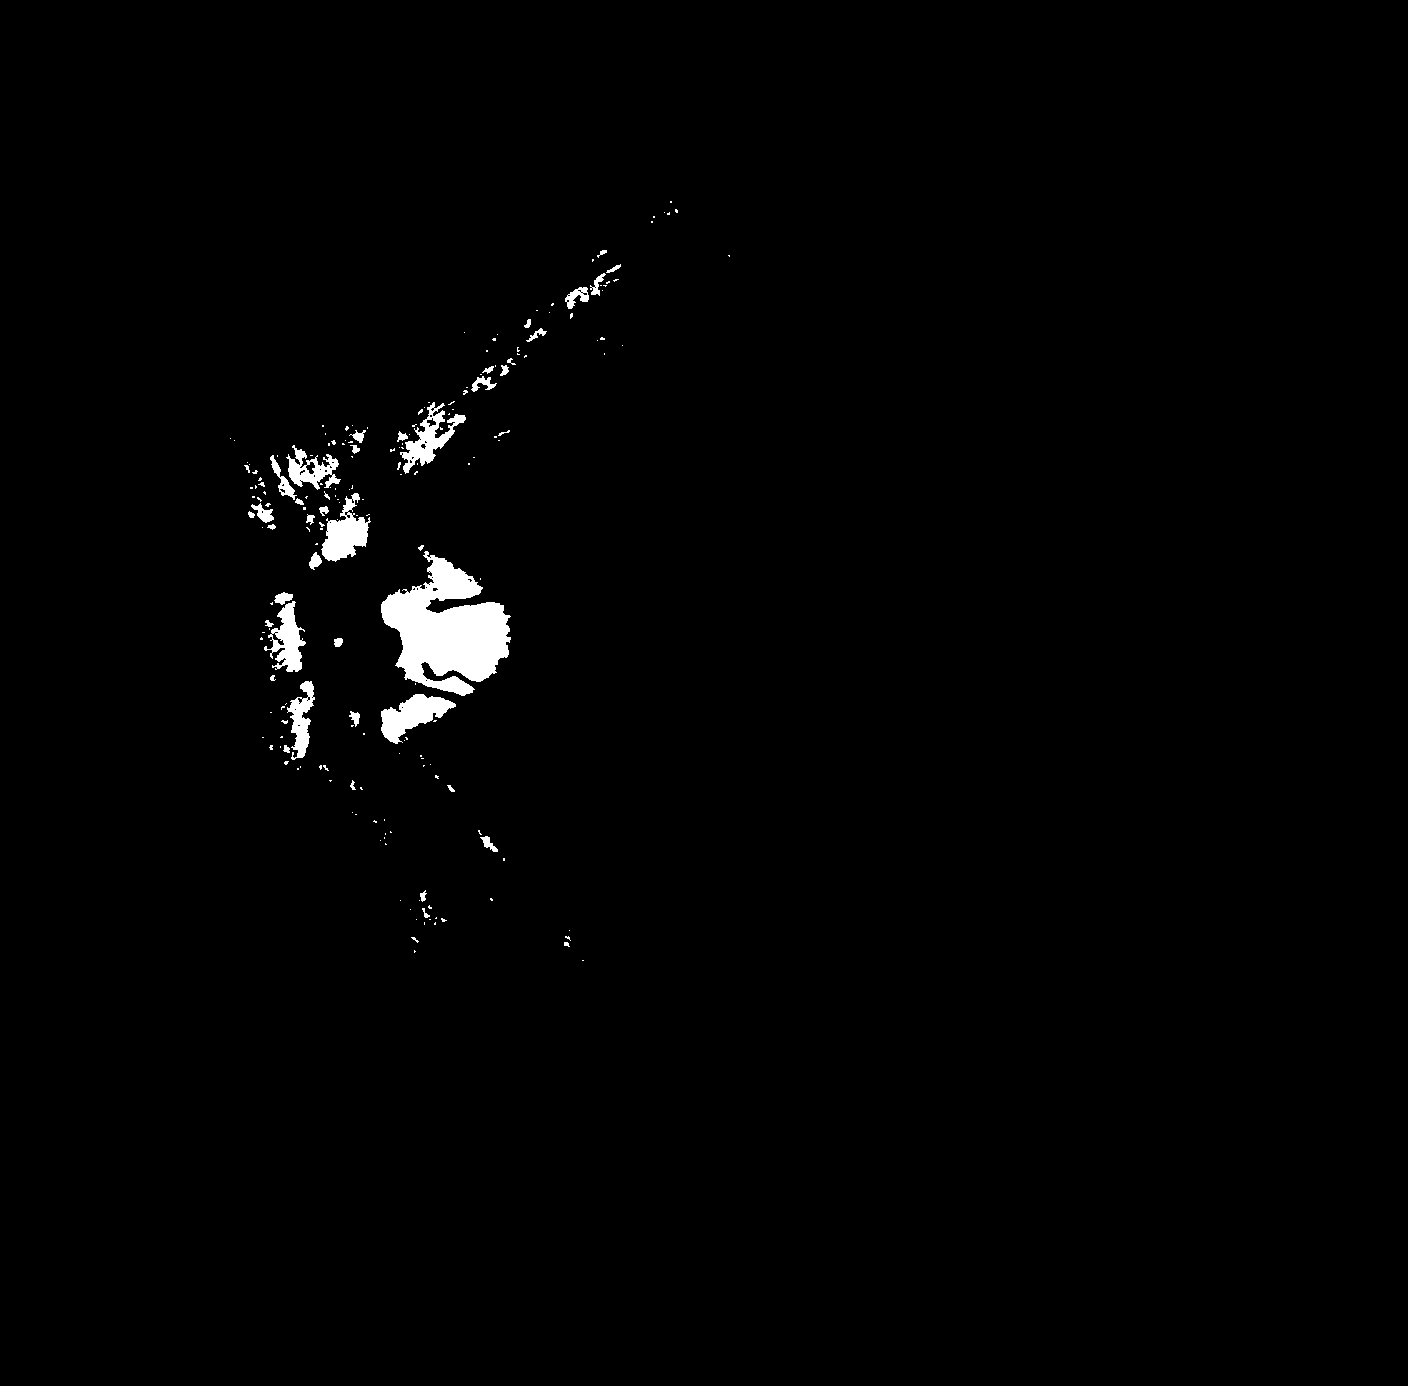
\includegraphics[width=50mm]{./Figures/cap4/disco/disco4.png}}
\caption{Umbralización.} \label{fig:disco_4}
\end{figure}

A la imagen umbralizada se le aplica una operación de erosión con  un elemento estructurante con forma de disco, con un tamaño de 12 píxeles, con el fin de acentuar la forma circular del disco óptico ( FIGURA \ref{fig:disco_5}). Como paso siguiente esta imagen se dilata  con un elemento estructurante en forma de disco, con un tamaño de 20 píxeles ( FIGURA \ref{fig:disco_6}).
\begin{figure}[H]
\centering
\subfigure[Imagen umbralizada.]{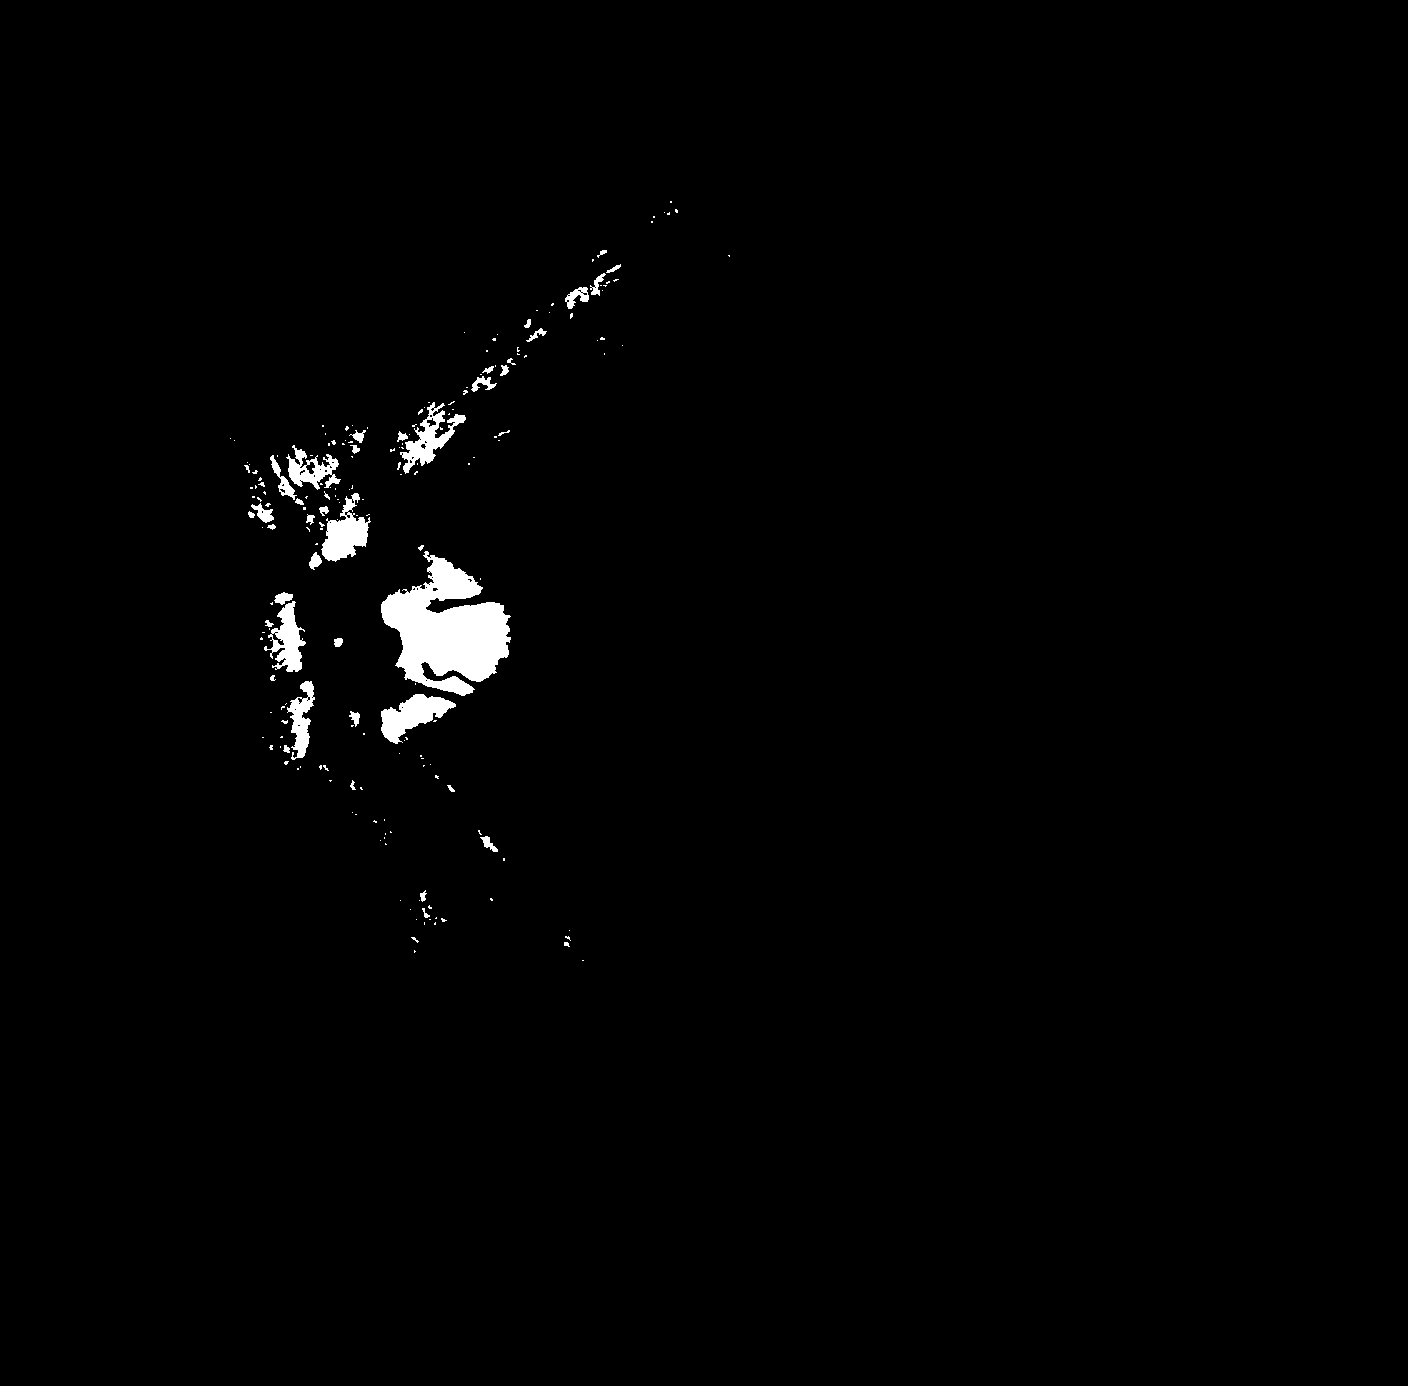
\includegraphics[width=50mm]{./Figures/cap4/disco/disco4.png}}
\subfigure[Imagen erosionada.]{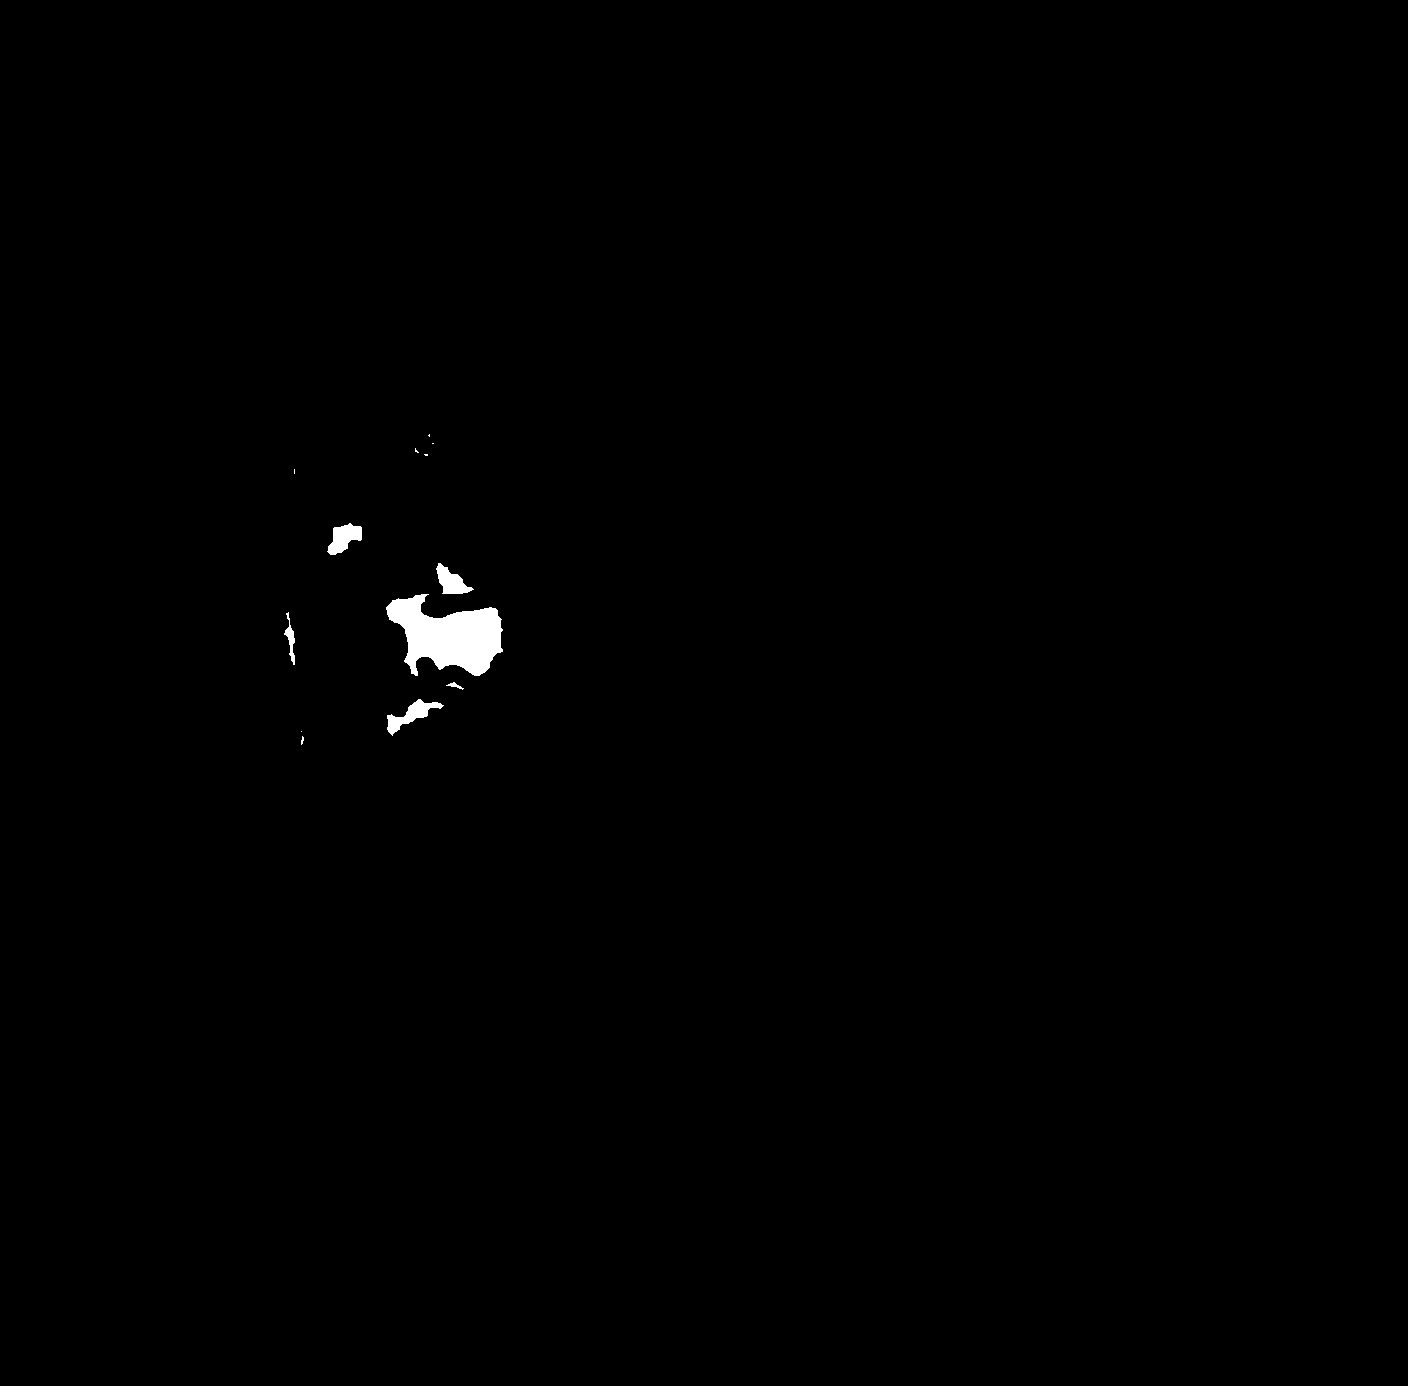
\includegraphics[width=50mm]{./Figures/cap4/disco/disco6.png}}
\caption{Erosión de imagen.} \label{fig:disco_5}
\end{figure}

\begin{figure}[H]
\centering
\subfigure[Imagen erosionada.]{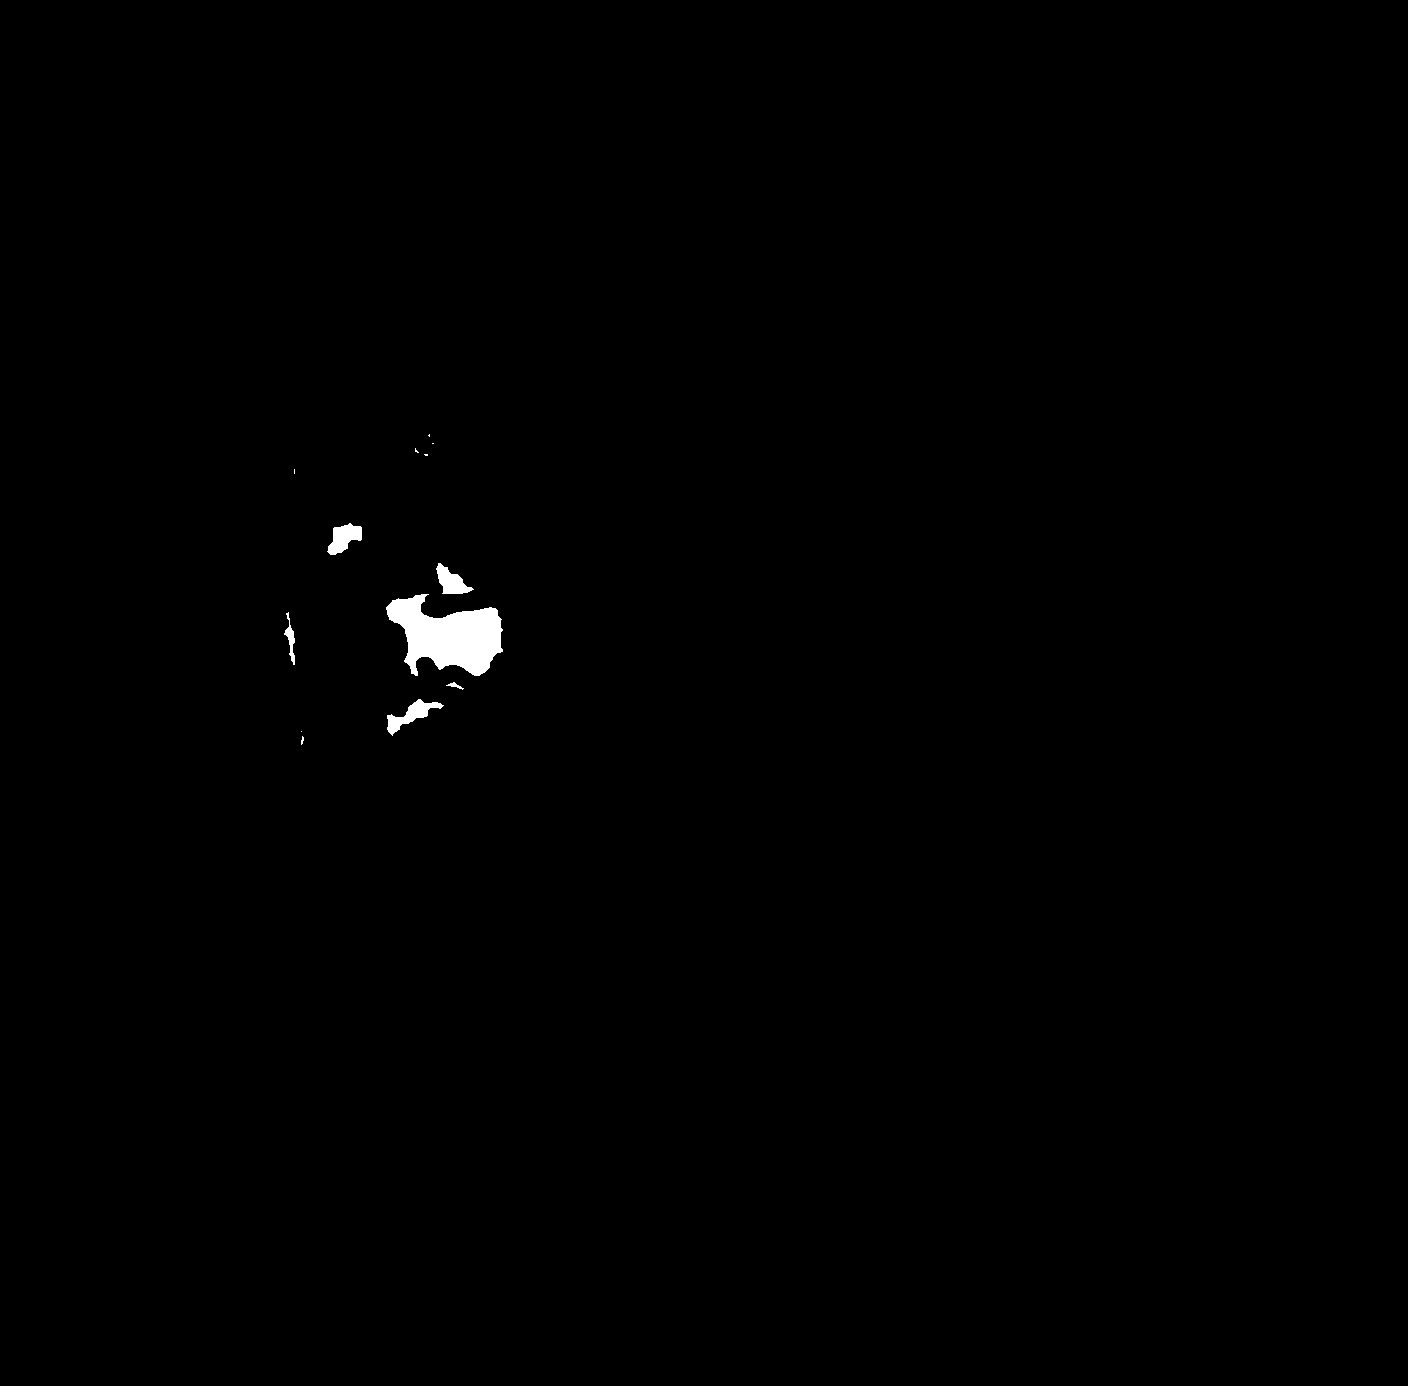
\includegraphics[width=50mm]{./Figures/cap4/disco/disco6.png}}
\subfigure[Imagen dilatada.]{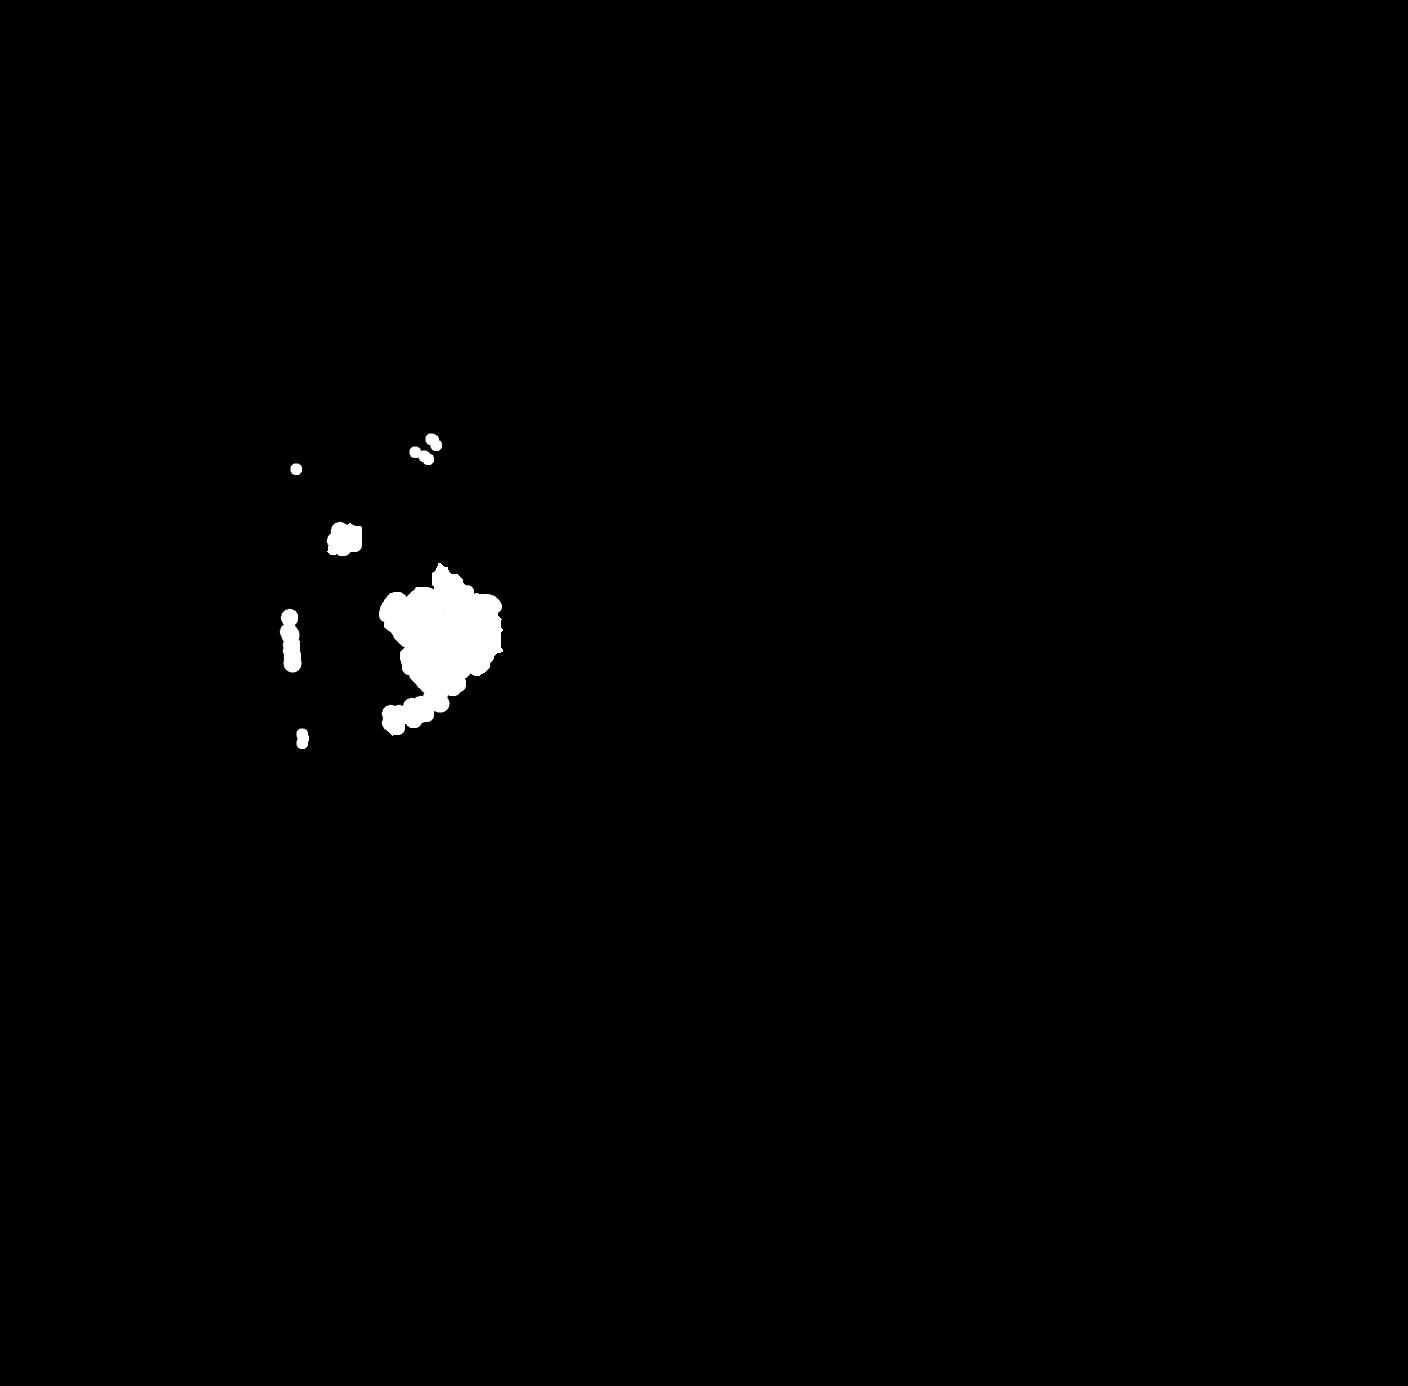
\includegraphics[width=50mm]{./Figures/cap4/disco/disco8.png}}
\caption{Dilatación de imagen.} \label{fig:disco_6}
\end{figure}

Asumiendo que el disco óptico es el objeto con mayor área, se eliminan todos los otros componentes conectados, dejando solo el elemento de mayor área, el cual es el  disco óptico$f_{do}$ ( FIGURA \ref{fig:disco_7}).

\begin{figure}[H]
\centering
\subfigure[Imagen dilatada.]{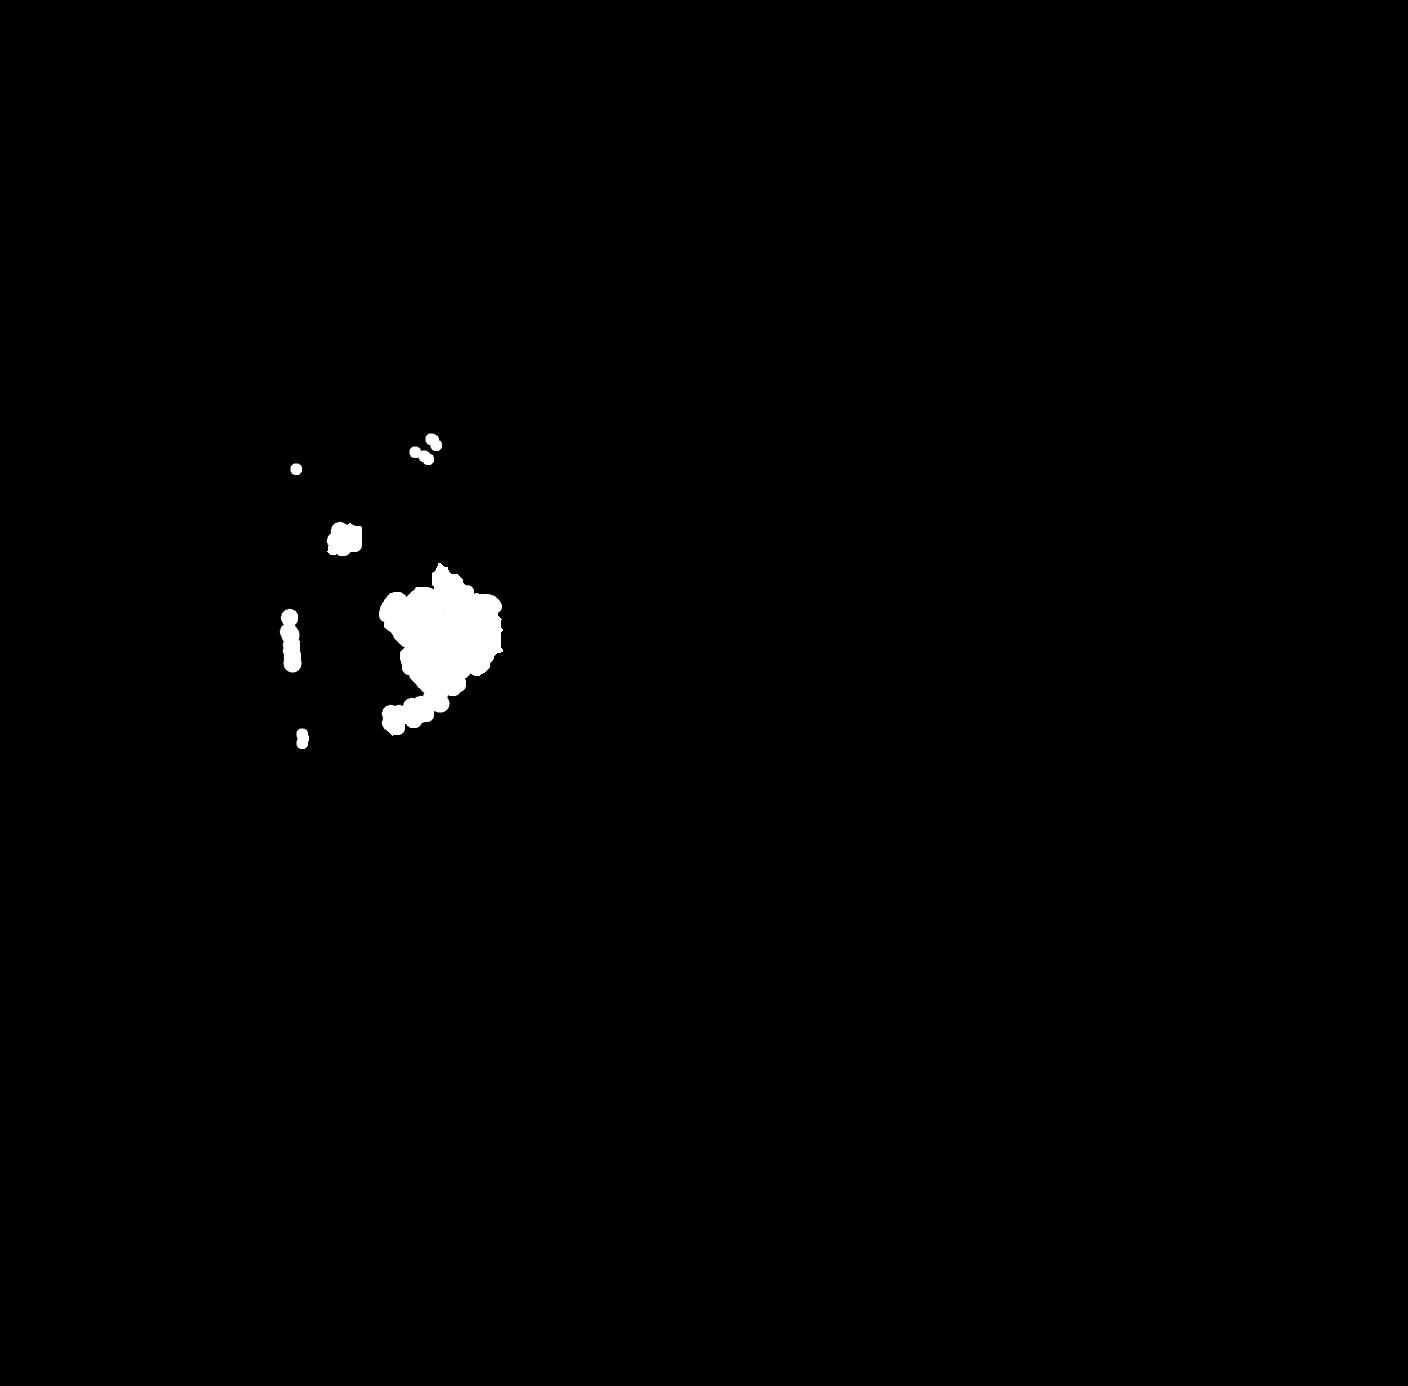
\includegraphics[width=50mm]{./Figures/cap4/disco/disco8.png}}
\subfigure[Imagen final $f_{do}$]{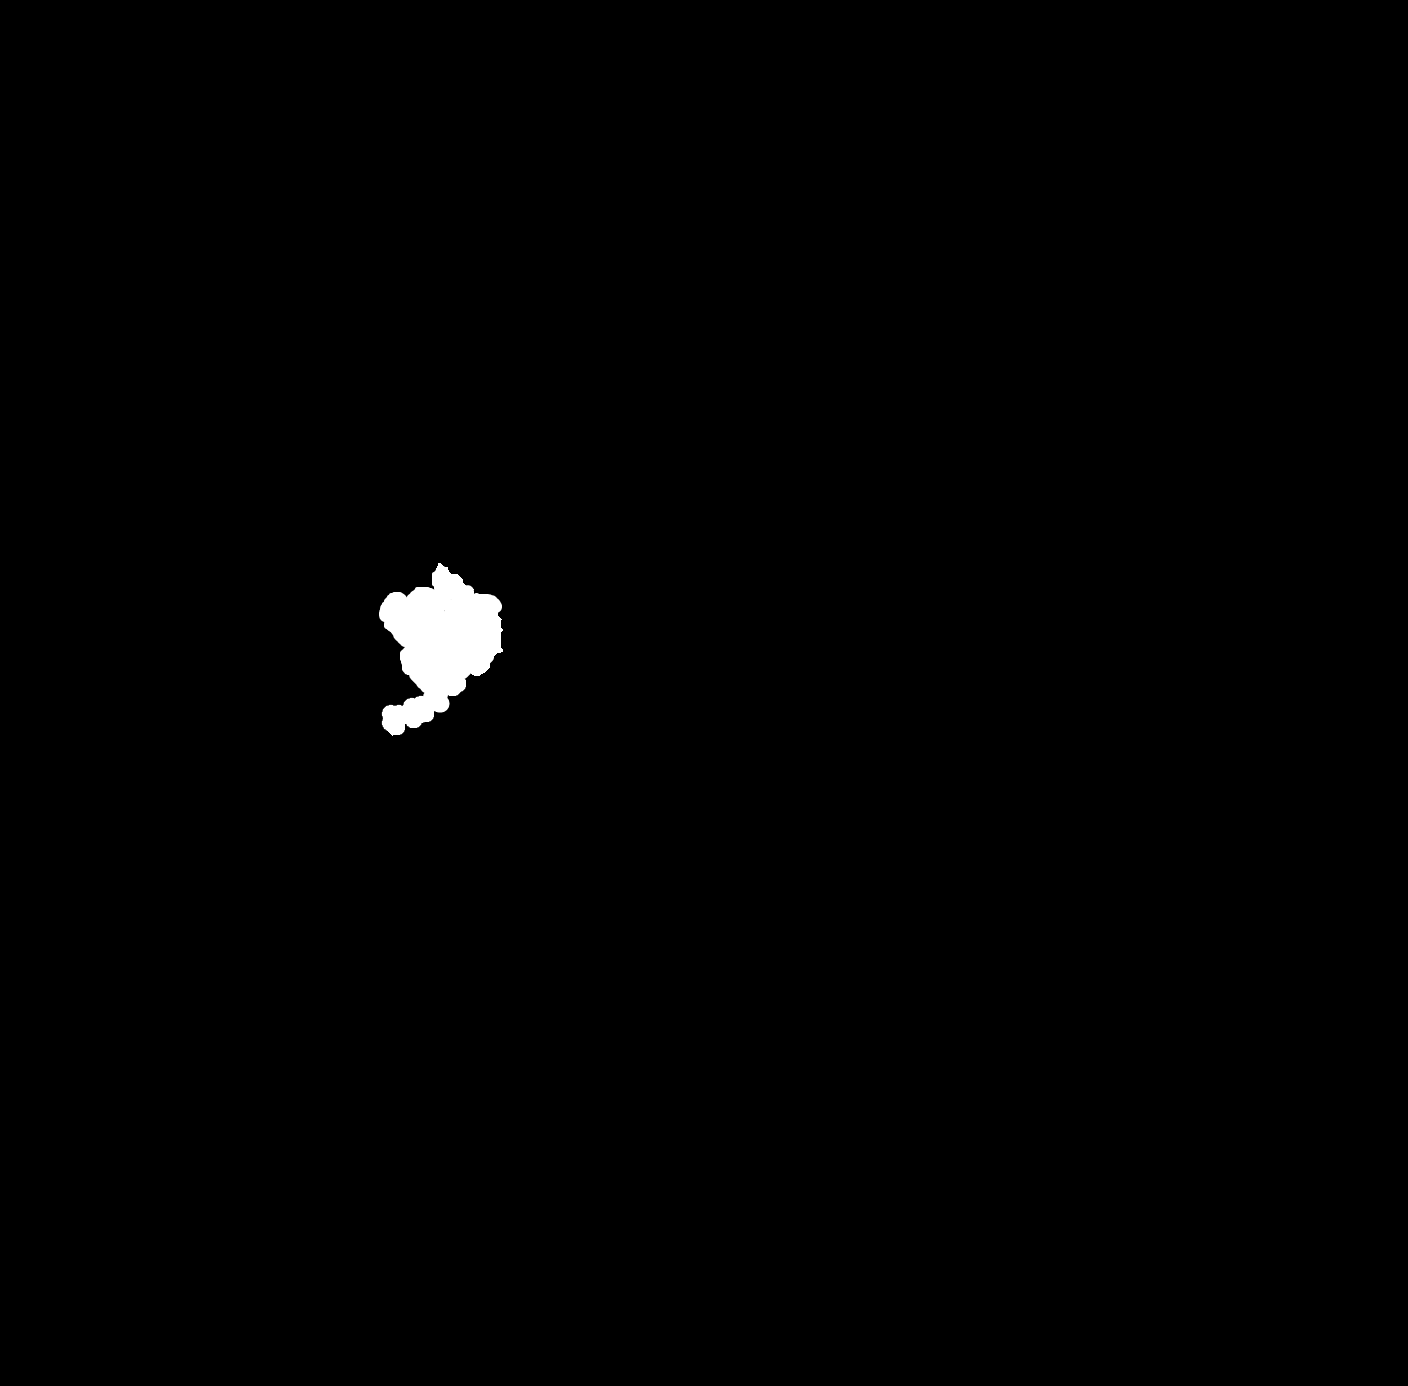
\includegraphics[width=50mm]{./Figures/cap4/disco/disco9.png}}
\caption{Imagen final del disco óptico.} \label{fig:disco_7}
\end{figure}


 La secuencia de pasos para la detección y segmentación de disco óptico puede verse en la FIGURA \ref{fig:diado}.
 % y  la secuencia de imágenes generadas son desplegadas en la FIGURA \ref{fig:discoptico}.

\begin{figure}[H]
	\centering
		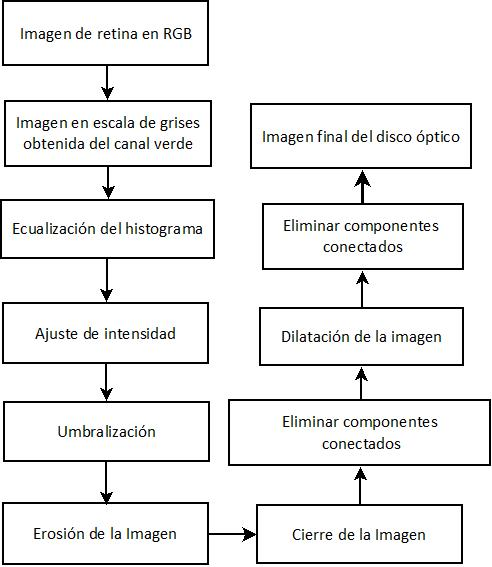
\includegraphics[width=0.7	\textwidth]{./Figures/cap4/dia_doo.jpeg}
	\caption{Diagrama de bloques de detección y segmentación de disco óptico.}
	\label{fig:diado}
\end{figure}

\subsubsection{Detección y segmentación del borde circular}
Con el objetivo de delimitar correctamente el área en la cual se encuentran los exudados duros, es  necesaria  la creación de un borde circular de las imágenes de retinas, ya que en algunas imágenes los bordes circulares son más claros y estos pueden ser confundidos por exudados duros.

 Para tal efecto la imagen original$f_{in}$ es umbralizada utilizando el método de Otsu de manera a tener una clara diferencia entre el área de la retina y el fondo de la imagen (FIGURA \ref{fig:borde_1}). Sobre esta imagen umbralizada se realiza la operación del gradiente morfológico utilizando un elemento estructurante con forma de disco de tamaño de 10 píxeles para obtener el borde circular (FIGURA \ref{fig:borde_2}). 
 
 \begin{figure}[H]
\centering
\subfigure[Imagen de retina.]{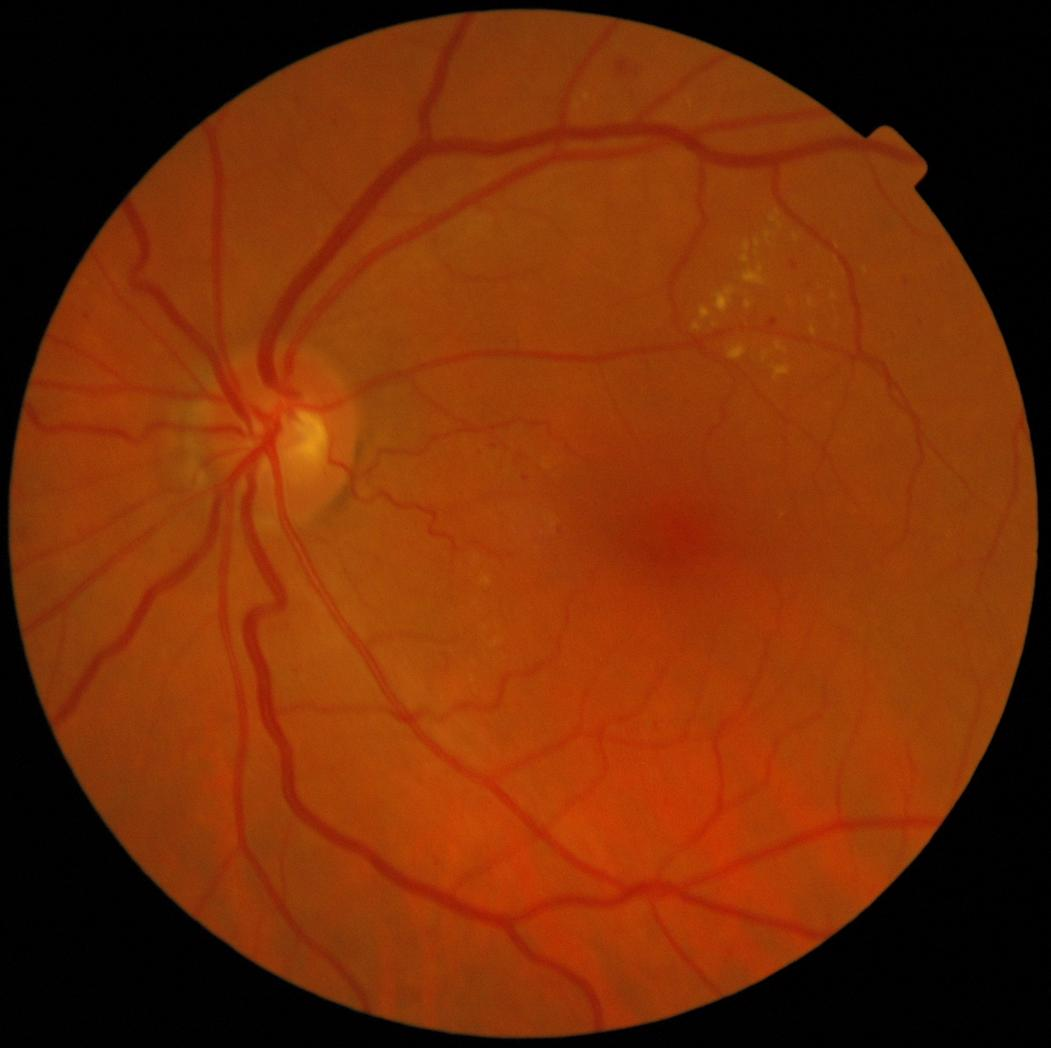
\includegraphics[width=50mm]{./Figures/cap4/vasos/vaso1.jpg}}
\subfigure[Imagen umbralizada.]{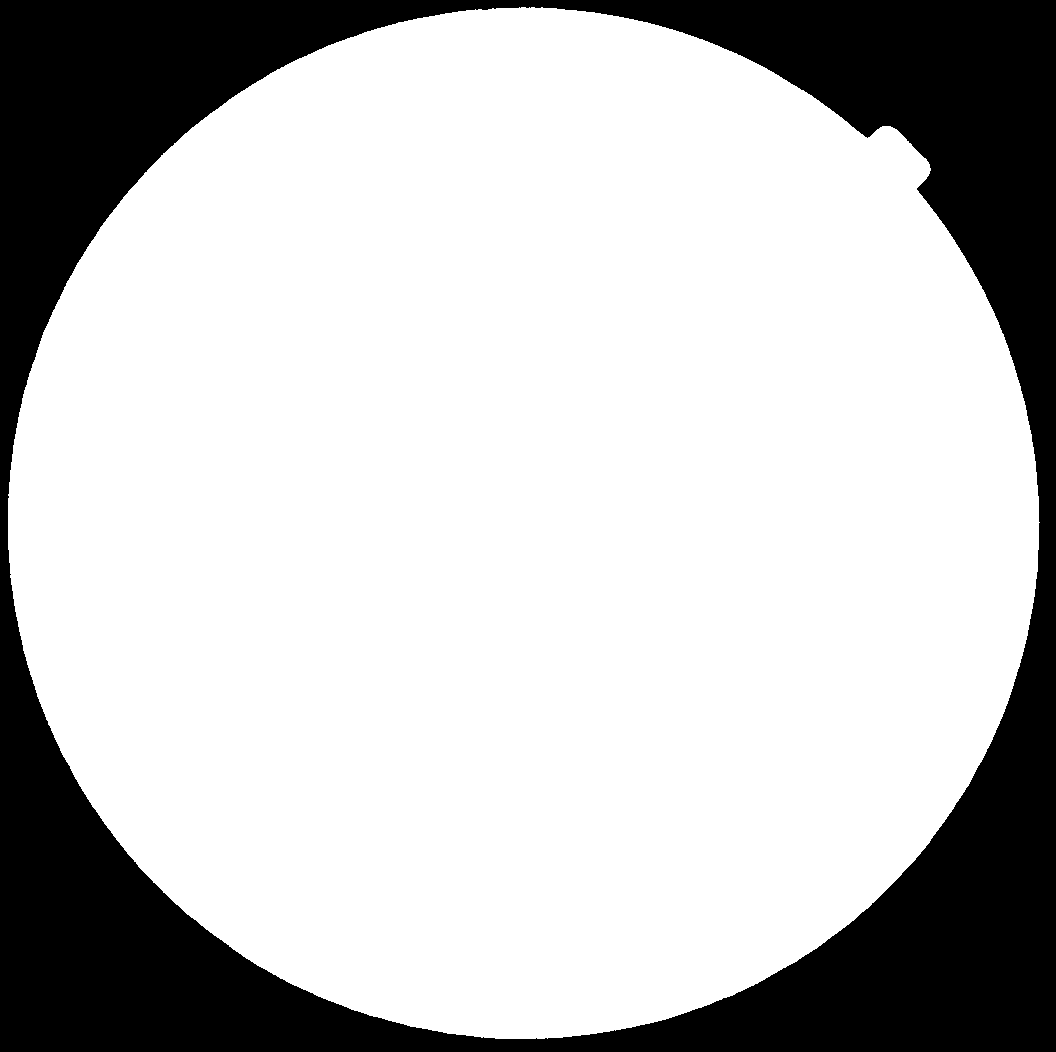
\includegraphics[width=50mm]{./Figures/cap3/borde/bordeUmb.png}}
\caption{Umbralización.} \label{fig:borde_1}
\end{figure}
 


 \begin{figure}[H]
\centering
\subfigure[Imagen umbralizada.]{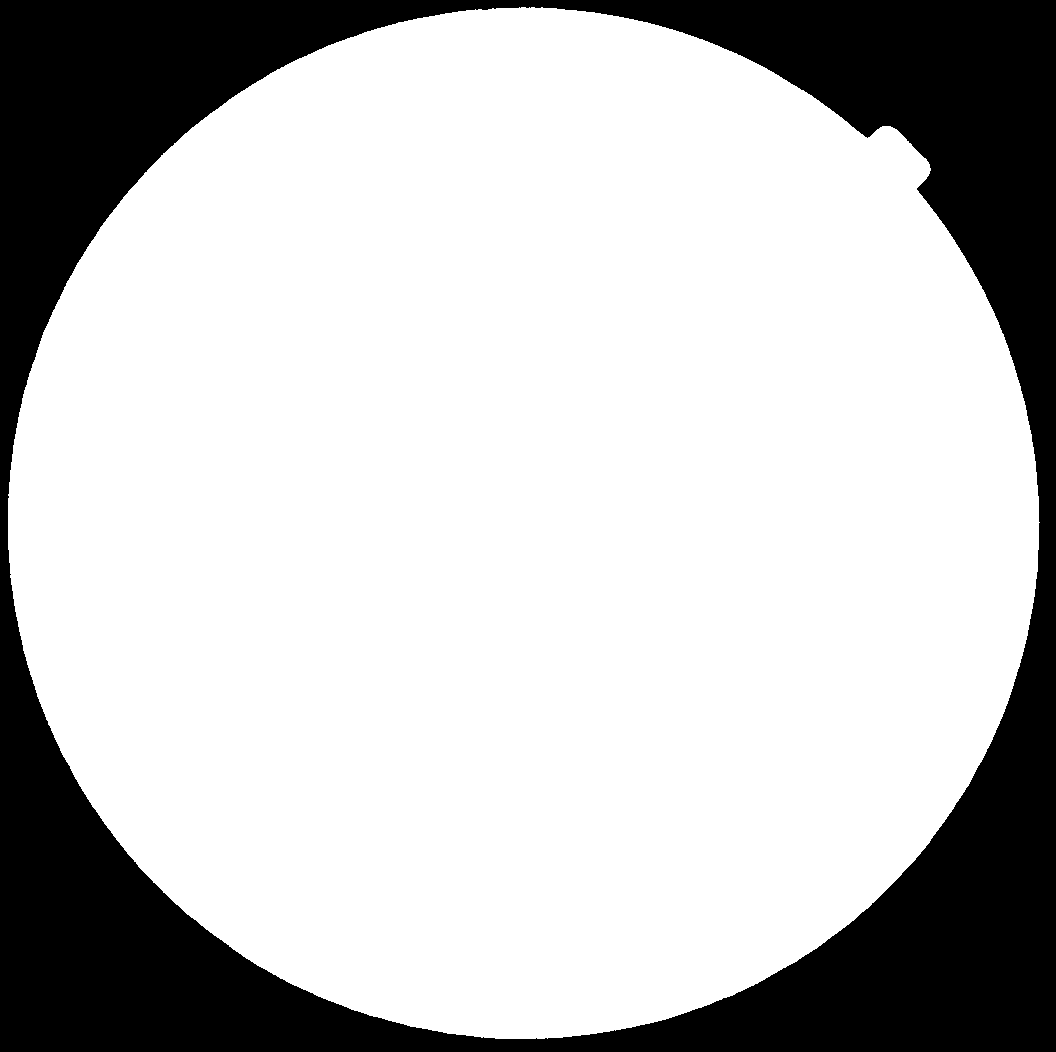
\includegraphics[width=50mm]{./Figures/cap3/borde/bordeUmb.png}}
\subfigure[Gradiente morfológico.]{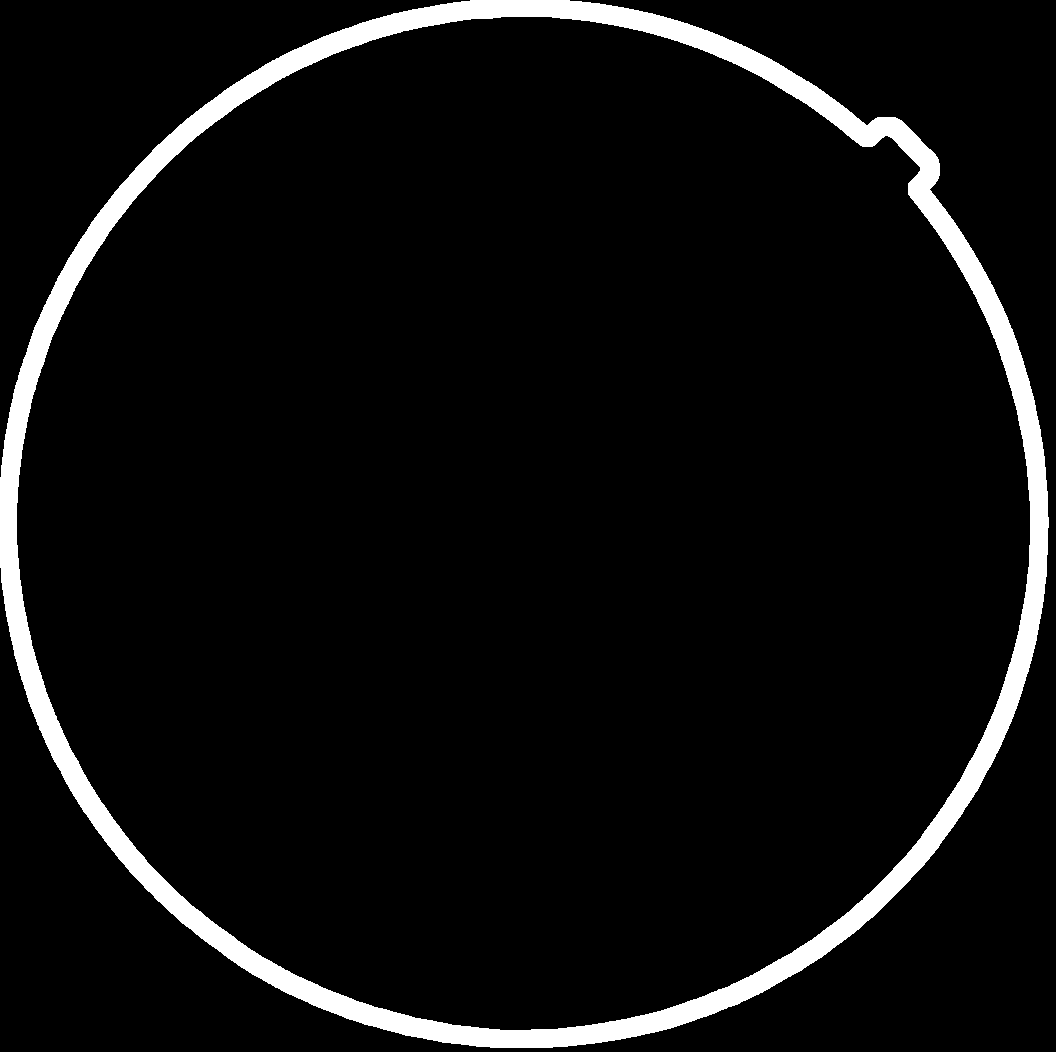
\includegraphics[width=50mm]{./Figures/cap3/borde/bordeRes.png}}
\caption{Gradiente morfológico.} \label{fig:borde_2}
\end{figure}

La secuencia de pasos para la detección y segmentación del borde circular puede verse en la FIGURA \ref{fig:bordeCircular}

 \begin{figure}[H]
	\centering
		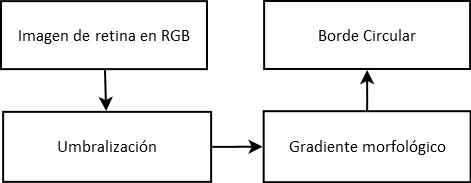
\includegraphics[width=0.7	\textwidth]{./Figures/cap4/bordeCircular.png}
	\caption{Diagrama de detección del Borde circular.}
	\label{fig:bordeCircular}
\end{figure}

\subsubsection{Detección y Segmentación de Exudados Duros}
Los exudados duros son lesiones claras, por lo que es más fácil detectarlos utilizando la intensidad de la imagen (FIGURA \ref{fig:exu_1}).
%Como primer paso del algoritmo, se obtiene el canal de intensidad de la imagen original$f_{in}$, luego 
%Sobre esta imagen
Se aplica un cierre morfológico con un elemento estructurante en forma de disco de 6 píxeles, eliminando pequeñas zonas que pueden ser identificadas como exudados debido a su variación de intensidad (FIGURA \ref{fig:exu_2}).
\begin{figure}[H]
\centering
\subfigure[Imagen de retina.]{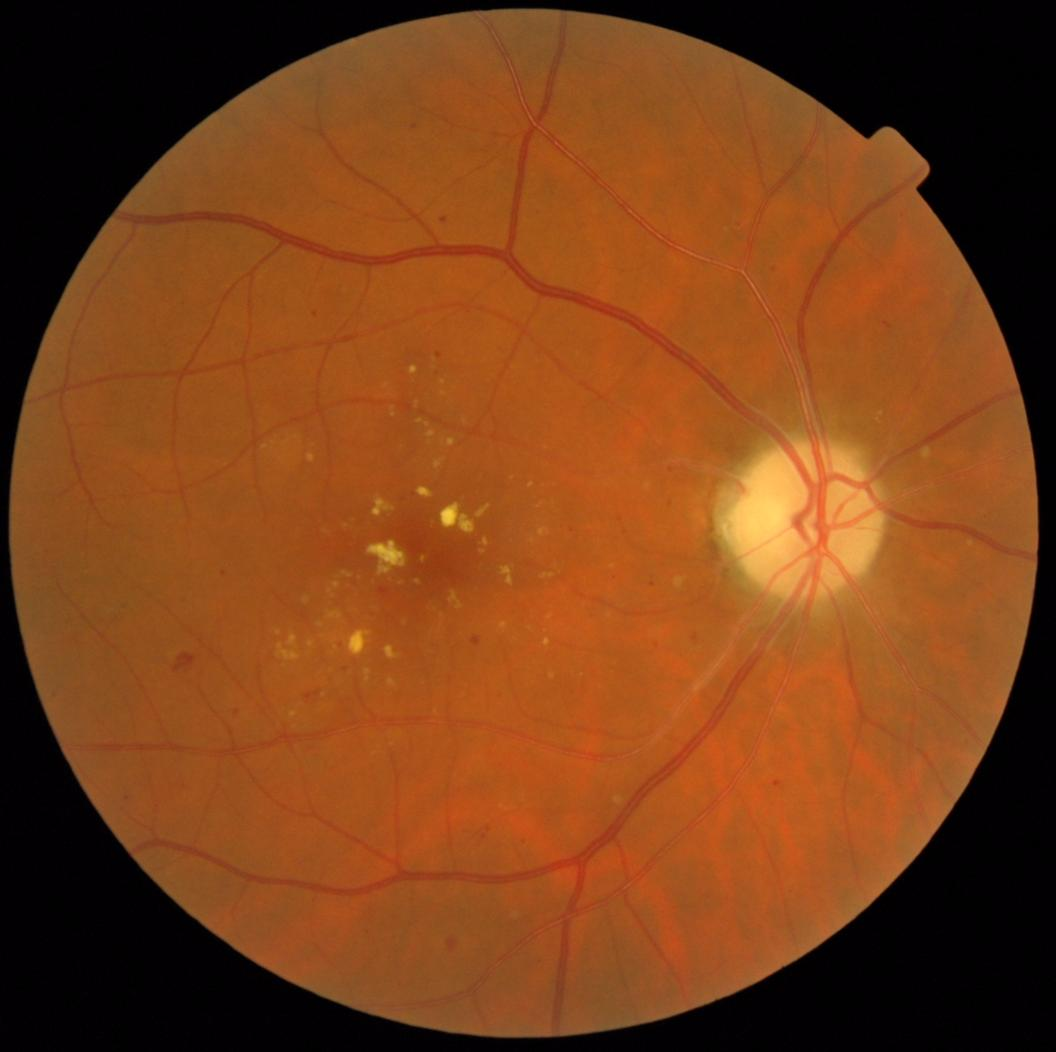
\includegraphics[width=50mm]{./Figures/cap3/exu/exu1.jpg}}
\subfigure[Intensidad de la Imagen.]{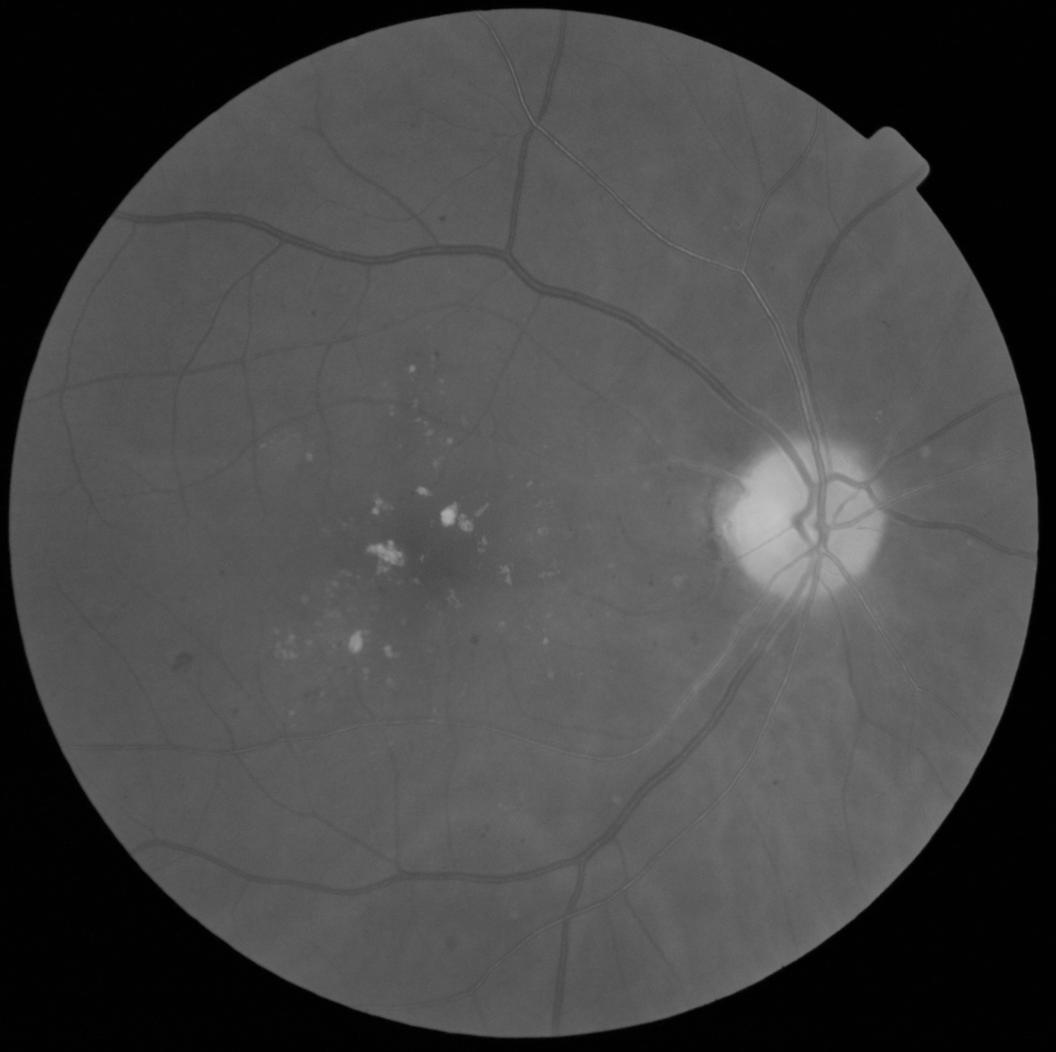
\includegraphics[width=50mm]{./Figures/cap3/exu/exu2.jpg}}
\caption{Intensidad de la imagen.} \label{fig:exu_1}
\end{figure}



\begin{figure}[H]
\centering
\subfigure[Intensidad de la Imagen.]{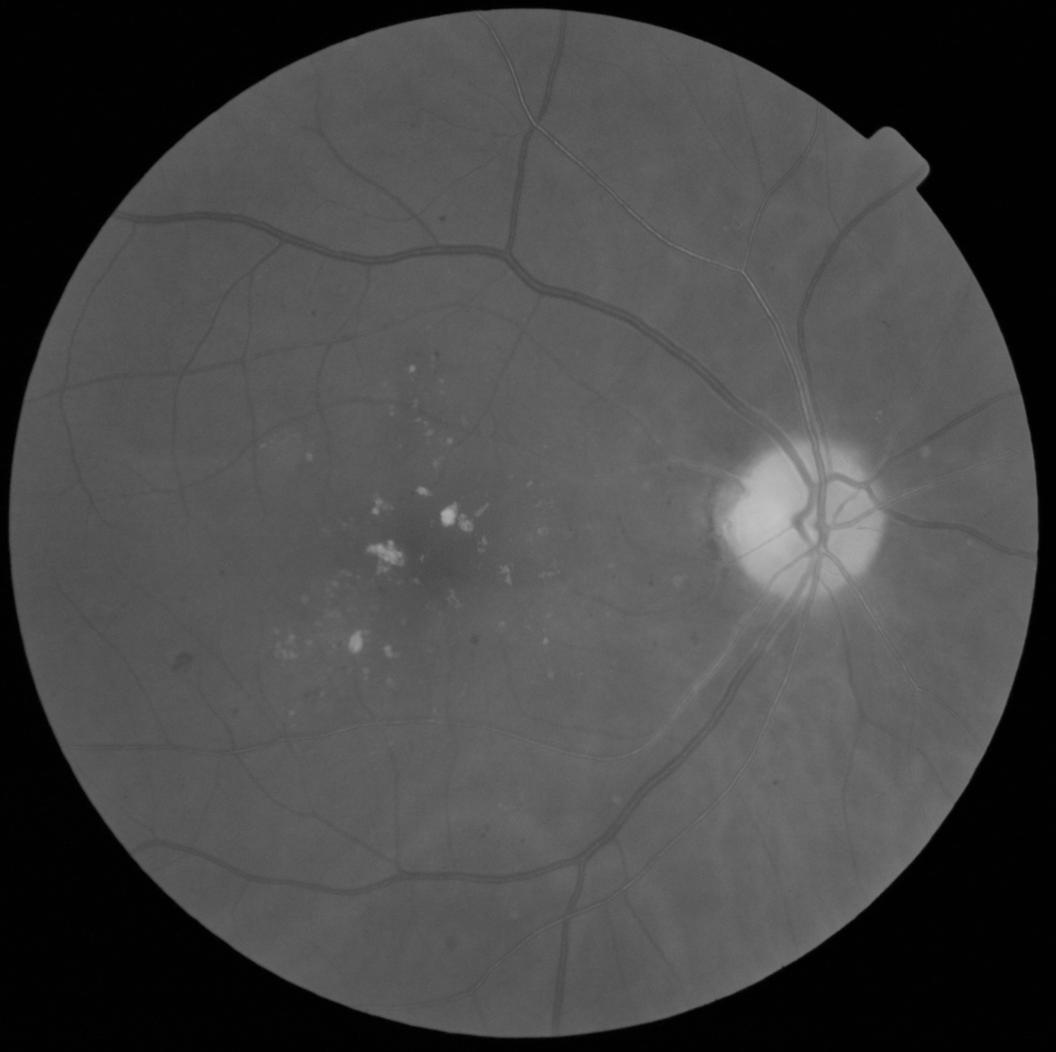
\includegraphics[width=50mm]{./Figures/cap3/exu/exu2.jpg}}
\subfigure[Cierre de imagen.]{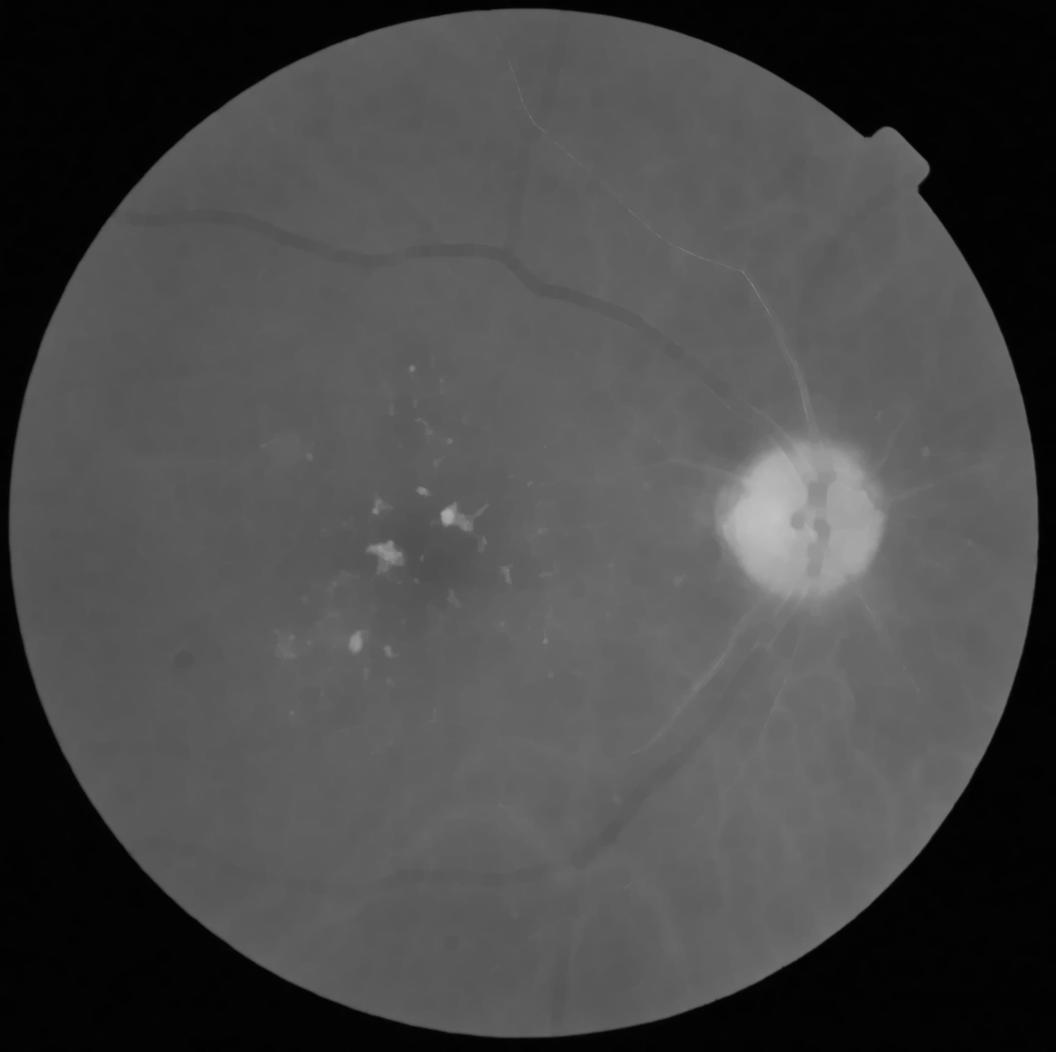
\includegraphics[width=50mm]{./Figures/cap3/exu/exu3.jpg}}

\caption{Cierre de imagen.} \label{fig:exu_2}
\end{figure}

Seguidamente, se obtiene las componentes brillantes aplicando la transformada de Top-Hat utilizando un elemento estructurante en forma de disco con un tamaño de 6 píxeles (FIGURA \ref{fig:exu_3}).
La imagen resultante es umbralizada por el método de entropía máxima (FIGURA \ref{fig:exu_4}).
\begin{figure}[H]
\centering
\subfigure[Cierre de Imagen.]{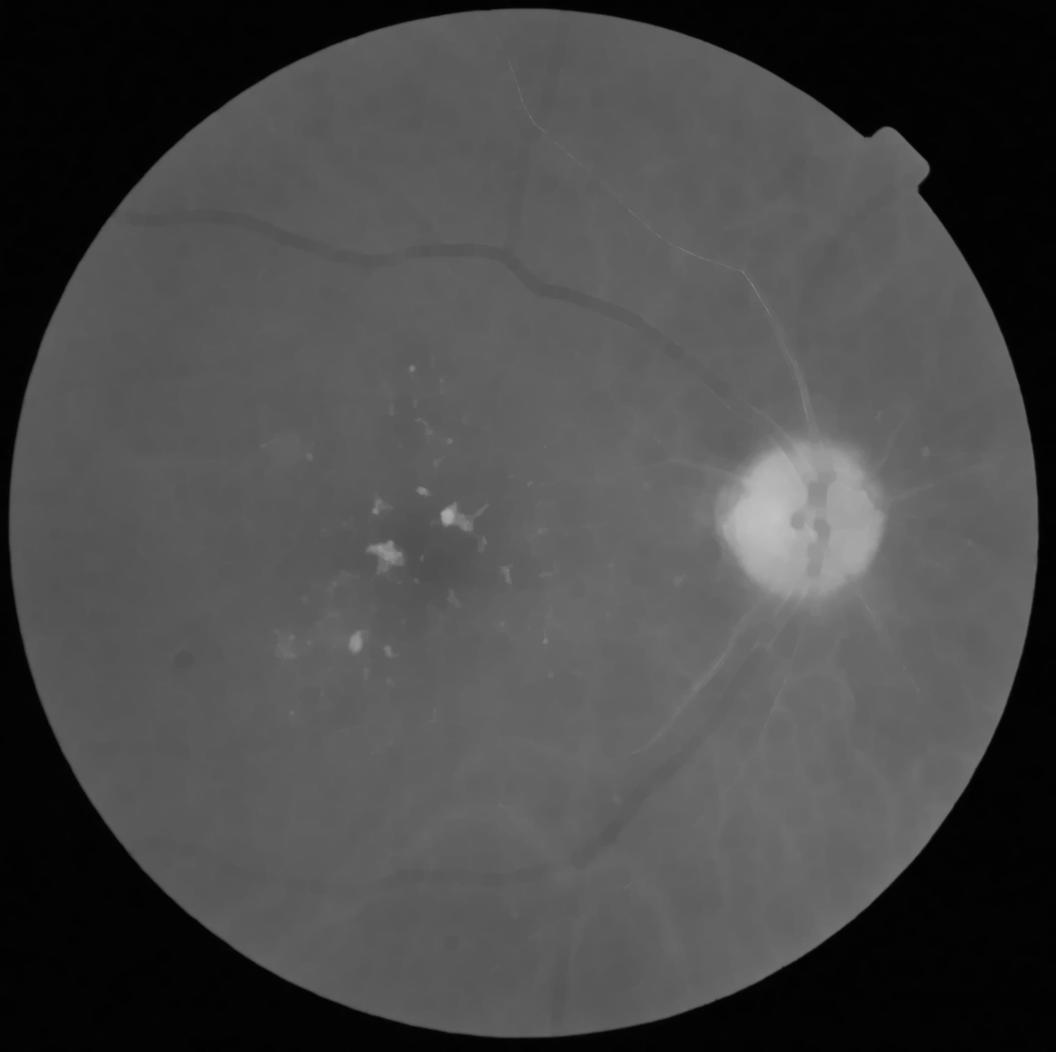
\includegraphics[width=50mm]{./Figures/cap3/exu/exu3.jpg}}
\subfigure[Top-hat de la imagen.]{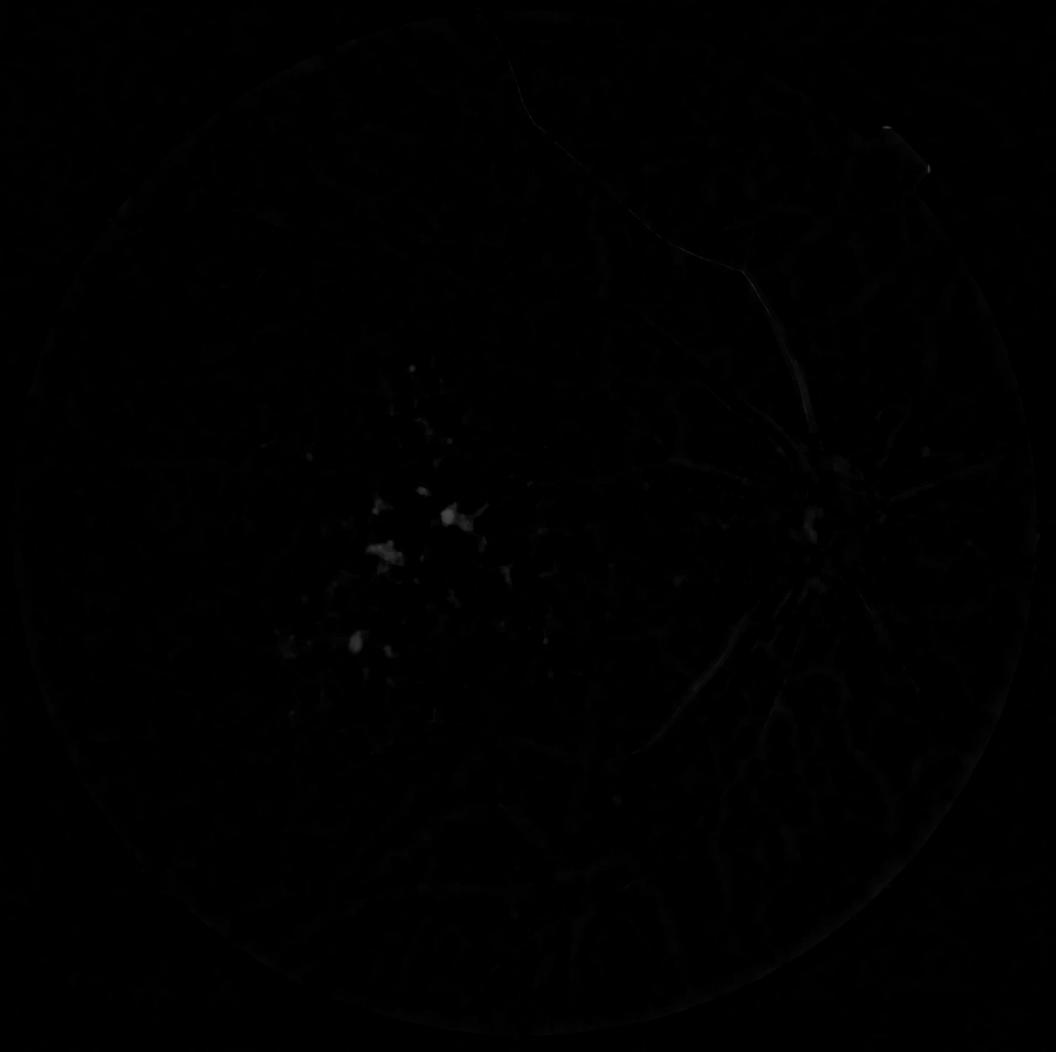
\includegraphics[width=50mm]{./Figures/cap3/exu/exu4.jpg}}

\caption{Top-hat de la imagen.} \label{fig:exu_3}
\end{figure}


\begin{figure}[H]
\centering
\subfigure[Top-hat de la imagen.]{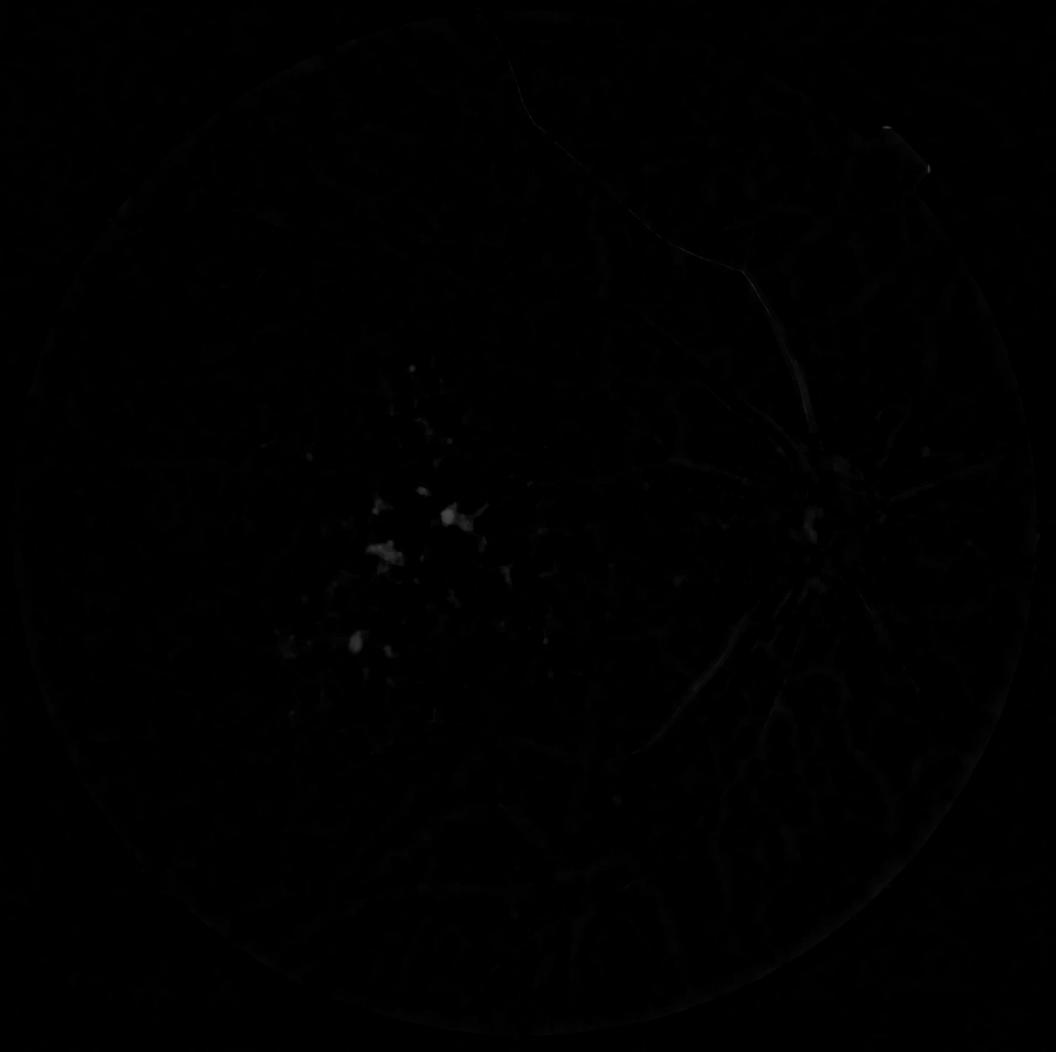
\includegraphics[width=50mm]{./Figures/cap3/exu/exu4.jpg}}
\subfigure[Umbralización de la imagen.]{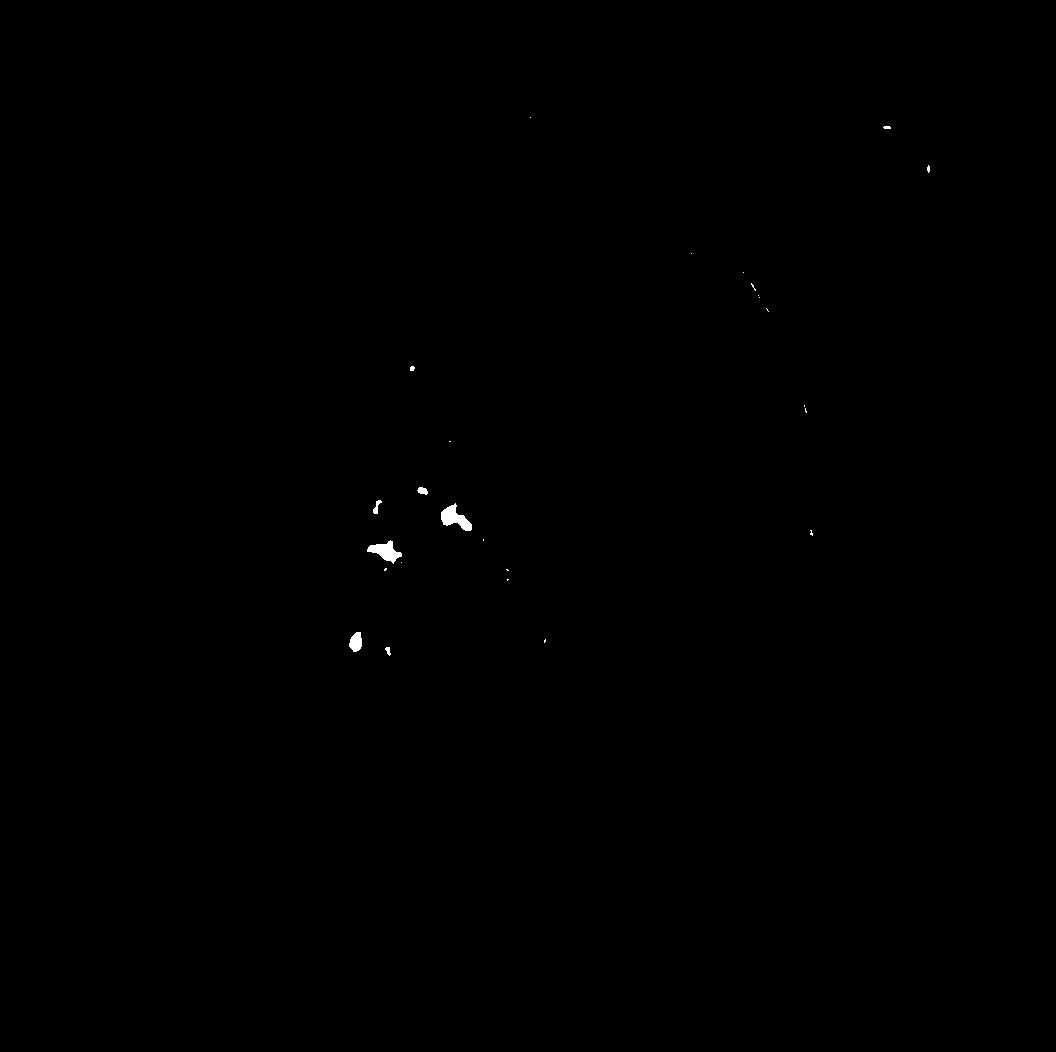
\includegraphics[width=50mm]{./Figures/cap3/exu/exu5.jpg}}

\caption{Umbralización de la imagen.} \label{fig:exu_4}
\end{figure}

De esta imagen se extraen las partes restantes de los vasos sanguíneos (FIGURA \ref{fig:exu_5}). Seguidamente se extrae el borde circular (FIGURA \ref{fig:exu_6}).

\begin{figure}[H]
\centering
\subfigure[Vasos sanguíneos.]{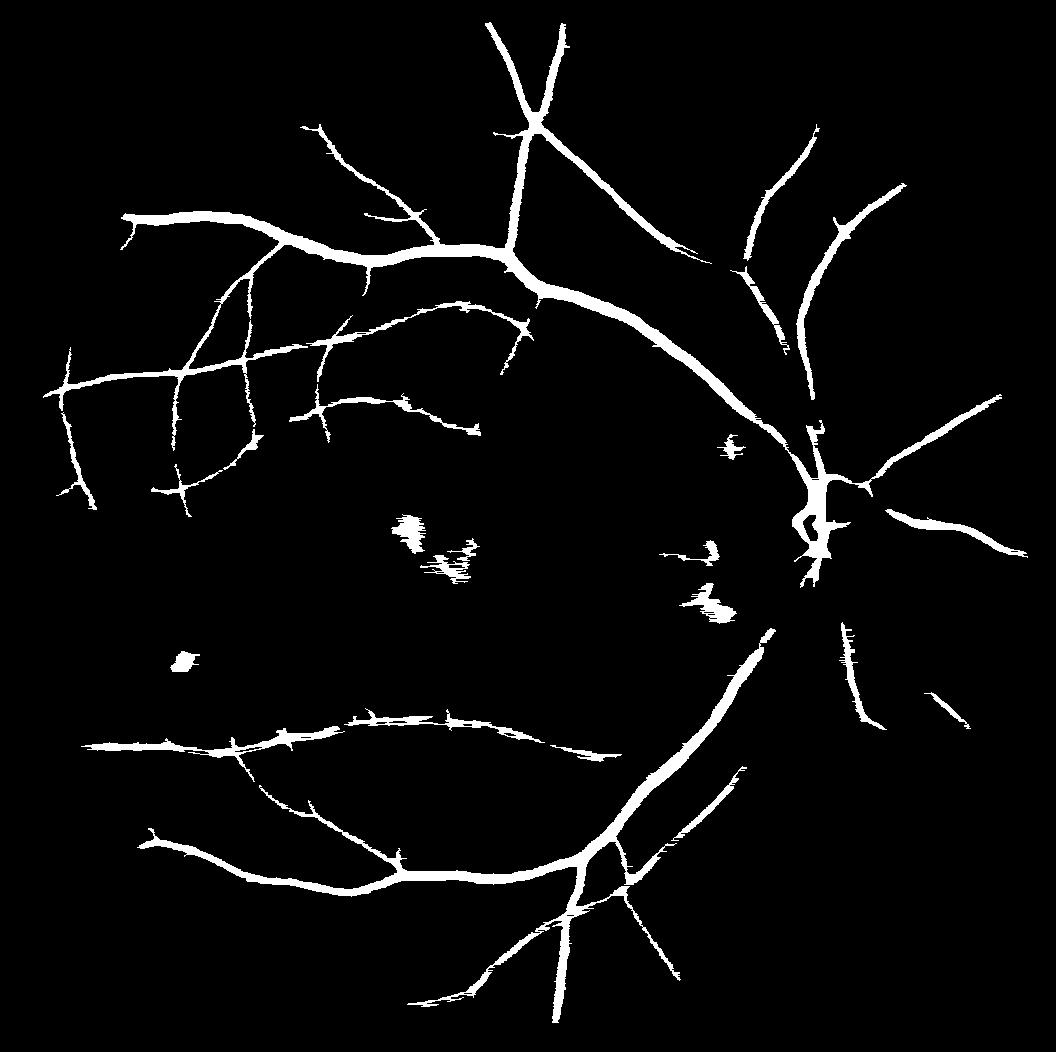
\includegraphics[width=50mm]{./Figures/cap3/exu/exuVena.jpg}}
\subfigure[Vasos sanguíneos extraídos.]{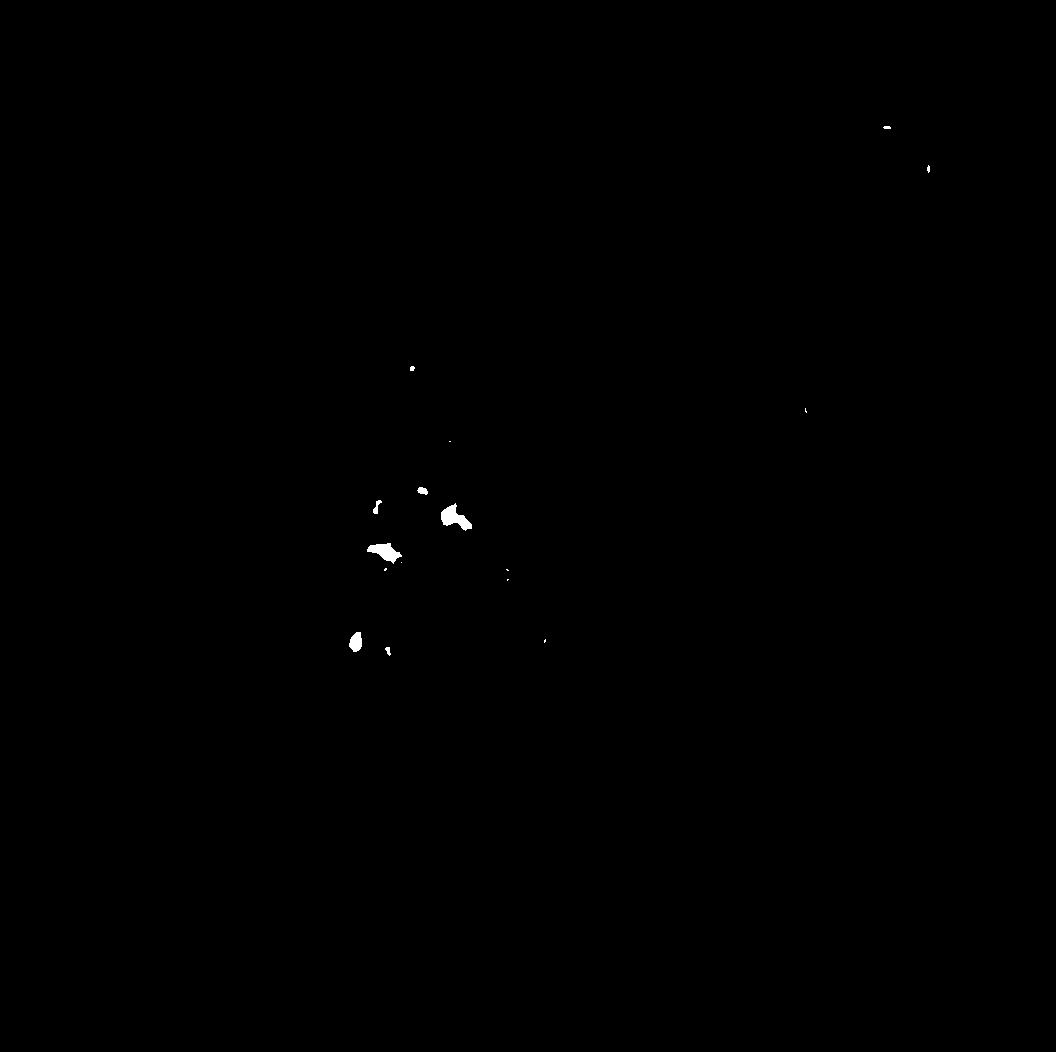
\includegraphics[width=50mm]{./Figures/cap3/exu/exuSinVena.jpg}}
\caption{Extracción de vasos sanguíneos.} \label{fig:exu_5}
\end{figure}


\begin{figure}[H]
\centering
\subfigure[Borde circular.]{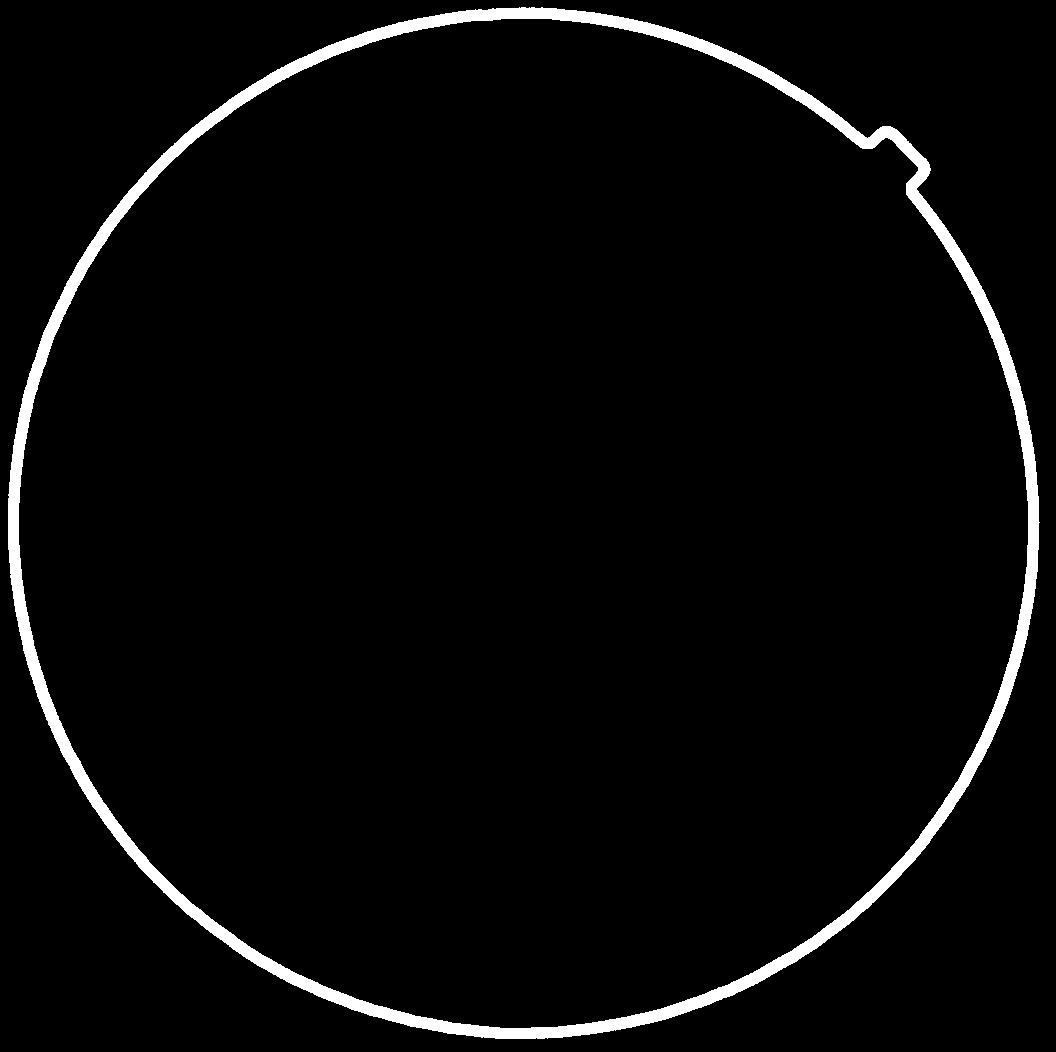
\includegraphics[width=50mm]{./Figures/cap3/exu/exuBorde.jpg}}
\subfigure[Borde circular extraídos.]{\includegraphics[width=50mm]{./Figures/cap3/exu/exuSinBorde.jpg}}
\caption{Extracción de borde circular.} \label{fig:exu_6}
\end{figure}
Por último, se extrae el disco óptico, obteniendo así la imagen final $f_{ed}$ (FIGURA \ref{fig:exu_7}).
\begin{figure}[H]
\centering
\subfigure[Disco óptico.]{\includegraphics[width=50mm]{./Figures/cap3/exu/exuDisco.jpg}}
\subfigure[Disco óptico extraído.]{\includegraphics[width=50mm]{./Figures/cap3/exu/exuSinDisco.jpg}}
\caption{Extracción de disco óptico.} \label{fig:exu_7}
\end{figure}
 
La secuencia de pasos para la detección y segmentación de exudados duros puede verse en la FIGURA \ref{fig:diaExu}.
%y la secuencia de imágenes generadas son desplegadas en la FIGURA \ref{fig:secExu}.
\begin{figure}[H]
	\centering
		\includegraphics[width=0.7	\textwidth]{./Figures/cap4/exudaEspa2.png}
	\caption{Diagrama de bloques de detección y segmentación de exudados duros.}
	\label{fig:diaExu}
\end{figure}

%\begin{figure}[H]
%	\centering
%		\includegraphics[width=0.7	\textwidth]{./Figures/cap4/secExu2.PNG}
%	\caption{Secuencia de imágenes de detección y segmentación de Exudados duros (a) Imagen de retina, (b) canal de intensidad de la imagen, (c) Cierre de imagen, (d) Transformada Top-Hat de imagen, (e) Imagen umbralizada, (f) Imagen de vasos sanguíneos, (g) Imagen de borde circular, (h) Imagen de disco óptico y (i) Imagen de  exudados duros segmentada $f_{ed}$}
%	\label{fig:secExu}
%\end{figure}

\subsection{Detección y segmentación de microaneurismas} 

Para la detección y segmentación de microaneurismas se obtiene del canal verde de la imagen de retina $f_{in}$ debido a que los microaneurismas contienen características más contrastadas en este canal (FIGURA \ref{fig:sec_ma_0}). 
\begin{figure}[H]
\centering
\subfigure[Imagen de retina.]{\includegraphics[width=50mm]{./Figures/cap4/vasos/vaso1.jpg}}
\subfigure[Canal verde de la imagen.]{\includegraphics[width=50mm]{./Figures/cap4/micro0.jpg}}
\caption{Canal verde de la imagen.} \label{fig:sec_ma_0}
\end{figure}

Con el objetivo de reducir el ruido de la imagen, aplicamos un filtro estadístico, específicamente el filtro de la mediana. Ver FIGURA \ref{fig:sec_ma_1}. Una vez filtrada esta imagen es normalizada (FIGURA \ref{fig:sec_ma_2}).


\begin{figure}[H]
\centering
\subfigure[ Canal verde de la imagen.]{\includegraphics[width=50mm]{./Figures/cap4/micro0.jpg}}
\subfigure[Imagen generada por el filtro de la mediana.]{\includegraphics[width=50mm]{./Figures/cap4/micro1.jpg}}
\caption{Filtro de la mediana.} \label{fig:sec_ma_1}
\end{figure}
%\subsubsection{Normalización de la intensidad}

\begin{figure}[H]
\centering
\subfigure[Filtro de la mediana.]{\includegraphics[width=50mm]{./Figures/cap4/micro1.jpg}}
\subfigure[Normalización de la intensidad.]{\includegraphics[width=50mm]{./Figures/cap4/micro2.jpg}}
\caption{Imagen con intensidad ajustada.} \label{fig:sec_ma_2}
\end{figure}

%\subsubsection{CLAHE}
Para finalizar el proceso de mejora se estira el contraste utilizando el algoritmo de CLAHE (FIGURA \ref{fig:sec_ma_3}). Luego esta imagen mejorada es erosionada por un elemento estructurante en forma de disco con un tamaño de 5 píxeles (FIGURA \ref{fig:sec_ma_4}).
\begin{figure}[H]
\centering
\subfigure[ Imagen con intensidad ajustada.]{\includegraphics[width=50mm]{./Figures/cap4/micro2.jpg}}
\subfigure[ Imagen ecualizada.]{\includegraphics[width=50mm]{./Figures/cap4/micro3.jpg}}
\caption{Ecualización del histograma.} \label{fig:sec_ma_3}
\end{figure}
 %\subsubsection{Imagen erosionada}
 

\begin{figure}[H]
\centering
\subfigure[Imagen ecualizada.]{\includegraphics[width=50mm]{./Figures/cap4/micro3.jpg}}
\subfigure[Imagen erosionada.]{\includegraphics[width=50mm]{./Figures/cap4/micro4.jpg}}
\caption{Erosión de una imagen.} \label{fig:sec_ma_4}
\end{figure}

 %\subsubsection{Resta de imágenes}
Después de esto se obtiene el borde, haciendo la diferencia entre la imagen mejorada y la erosionada (FIGURA \ref{fig:sec_ma_5}).  %\subsubsection{Imagen umbralizada}
 Esta imagen es umbralizada en intensidad para generar una nueva imagen conteniendo los posibles microaneurismas (FIGURA \ref{fig:sec_ma_6}).
 \begin{figure}[H]
\centering
\subfigure[Imagen ecualizada.]{\includegraphics[width=50mm]{./Figures/cap4/micro4.jpg}}
\subfigure[Resta de imágenes.]{\includegraphics[width=50mm]{./Figures/cap4/micro66.jpg}}
\caption{Resta de imágenes.} \label{fig:sec_ma_5}
\end{figure}


 \begin{figure}[H]
\centering
\subfigure[Imagen a umbralizar.]{\includegraphics[width=50mm]{./Figures/cap4/micro66.jpg}}
\subfigure[Imagen umbralizada.]{\includegraphics[width=50mm]{./Figures/cap4/micro6.jpg}}
\caption{Umbralización.} \label{fig:sec_ma_6}
\end{figure}
 
 %\subsubsection{componentes conectados}
 De esta imagen se mantienen los componentes conectados en un rango de área entre 65 y 200 píxeles (FIGURA \ref{fig:sec_ma_7}).  Finalmente, se aplica un cierre con un disco para sobresaltar la forma circular de los componentes conectados (FIGURA \ref{fig:sec_ma_8}).
 
 \begin{figure}[H]
\centering
\subfigure[ Imagen umbralizada.]{\includegraphics[width=50mm]{./Figures/cap4/micro6.jpg}}
\subfigure[Imagen con componentes conectados eliminados.]{\includegraphics[width=50mm]{./Figures/cap4/micro9.jpg}}
\caption{Componentes conectados.} \label{fig:sec_ma_7}
\end{figure}
 %\subsubsection{Cierre de imagen}
 


 \begin{figure}[H]
\centering
\subfigure[Imagen binaria.]{\includegraphics[width=50mm]{./Figures/cap4/micro9.jpg}}
\subfigure[Cierre de imagen.]{\includegraphics[width=50mm]{./Figures/cap4/micro10.jpg}}
\caption{Cierre de imagen.} \label{fig:sec_ma_8}
\end{figure} 
 
 %\subsubsection{Imágenes con componentes de forma circular $f_{ma}$}
Se obtienen los componentes conectados de forma circular que son los microaneurismas detectados en  la imagen final $f_{ma}$ (FIGURA \ref{fig:sec_ma_9}).

 \begin{figure}[H]
\centering
\subfigure[Imagen erosionada.]{\includegraphics[width=50mm]{./Figures/cap4/micro10.jpg}}
\subfigure[Imagen final con MA.]{\includegraphics[width=50mm]{./Figures/cap4/micro12.jpg}}
\caption{Imágenes con componentes de forma circular $f_{ma}$} \label{fig:sec_ma_9}
\end{figure}

La secuencia de pasos para la detección y segmentación de microaneurismas puede verse en la FIGURA \ref{fig:diaMa}.
%y la secuencia de imágenes generadas son desplegadas en la FIGURA \ref{fig:secMa}.

\begin{figure}[H]
	\centering
		\includegraphics[width=0.7	\textwidth]{./Figures/cap4/dia_ma.png}
	\caption{Diagrama de bloques de detección y segmentación de microaneurismas.}
	\label{fig:diaMa}
\end{figure}


%\begin{figure}[H]
%	\centering
%		\includegraphics[width=0.7	\textwidth]{./Figures/cap4/sec_ma.png}
%	\caption{Secuencia de imágenes de detección y segmentación de Micro aneurismas (a) Imagen de Retina, (b) Canal verde de la imagen, (c) Imagen generada por el filtro de la mediana, (d) Imagen con intensidad ajustada, (e) Imagen ecualizada, (f) Imagen erosionada, (g) Resta de imágenes, (h) Imagen umbralizada, (i) Imagen sin componentes conectados y (j) Imágenes con componentes de forma circular $f_{ma}$.}
%	\label{fig:secMa}
%\end{figure}

\section{Módulo 2: Extracción de características}
Una vez finalizada la etapa de segmentación es necesario extraer las áreas de interés de las imágenes, para este trabajo el vector característica utilizado está determinado por las siguientes características:
\begin{itemize}
\item Área de vasos sanguíneos ($C_{vs}$).
\item Área de exudados duros ($C_{ed}$).
\item Área de microaneurismas ($C_{ma}$).
\end{itemize}

\nomenclature[49]{$f_{vs}$}{Imagen binaria final de vasos sanguíneos segmentados.}
\nomenclature[50]{$f_{ed}$}{Imagen binaria final de exudados duros segmentados.}
\nomenclature[51]{$f_{ma}$}{Imagen binaria final de microaneurismas segmentados.}

Las cuales se obtienen sumando los píxeles de las imágenes $f_{vs}$, $f_{ed}$ y $f_{ma}$.

%La sumatoria de las áreas de los componentes conectados $A$ se define como:

%\begin{equation}
%\label{eq:AreaObjetoSeg}
%A=\sum_{i=0}^{m} \sum_{j=0}^{n} f(i,j)
%\end{equation}

\begin{equation}
\label{eq:AreaObjetoSeg1}
C_{vs}=\sum_{i=0}^{i=M-1} \sum_{j=0}^{j=N-1} f_{vs}(i,j)
\end{equation}

\nomenclature[52]{$C_{vs}$}{Área de los vasos sanguíneos calculado a partir de la imagen binaria $f_{vs}$.}
\nomenclature[53]{$C_{ed}$}{Área de los exudados duros calculado a partir de la imagen binaria $f_{ed}$.}
\nomenclature[54]{$C_{ma}$}{Área de los microaneurismas calculado a partir de la imagen binaria  $f_{ma}$.}


\begin{equation}
\label{eq:AreaObjetoSeg2}
C_{ed}=\sum_{i=0}^{i=M-1} \sum_{j=0}^{j=N-1} f_{ed}(i,j)
\end{equation}

\begin{equation}
\label{eq:AreaObjetoSeg3}
C_{ma}=\sum_{i=0}^{i=M-1} \sum_{j=0}^{j=N-1} f_{ma}(i,j)
\end{equation}

En ese contexto, el vector de características $x$ está conformado por $C_{vs}$, $C_{ed}$ y $C_{ma}$, esto es $x=\{C_{vs},C_{ed},C_{ma}\}$.
%El área $A$ se calcula sumando todos los píxeles de la imagen e indica la suma de las áreas de los objetos segmentados. 

\section{Módulo 3: Clasificación}
Se realiza la clasificación de imágenes por el clasificador binario Support Vector Machine (SVM) \cite{cortes1995support}, el mismo ya alcanza un nivel de  exactitud favorable luego de tres o cuatro rondas de buena retroalimentación. Básicamente el clasificador SVM recibe un conjunto de características de entrenamiento $D=\{x,y\}$, donde $x$ es el conjunto de vectores de características e $y$ es el conjunto de etiquetas, cada etiqueta pertenece a una de dos categorías, en nuestro caso 0 para una retina sana y 1 en caso de ser una retina con retinopatía diabética, a partir del conjunto de entrenamiento se construye un modelo que posteriormente será usado para clasificar las imágenes de prueba.%Considerando los resultados obtenidos según el clasificador, en el capítulo siguiente se realiza un análisis de los mismos en base a las métricas de comparación. 


\section{Resumen}


En este capítulo se detalla la manera de obtener un diagnóstico a partir de una imagen de retina. Para lograr entender el funcionamiento de la metodología propuesta antes se debe entender como funciona cada uno de sus módulos. El primero de ellos es el módulo de detección y segmentación, en este módulo se describe los pasos realizados sobre la imagen de entrada y obtener a partir de esos pasos imágenes binarias segmentadas. En este módulo se comentan tres segmentaciones principales que son la de vasos sanguíneos, exudados duros y microaneurismas y dos segmentaciones secundarias que son  la de borde circular y disco óptico.
 En el segundo módulo se realiza la extracción de características de las imágenes segmentadas. El proceso se reduce a hallar el área en píxeles de las patologías y estructuras del ojo segmentadas.
 Como último paso se hace la clasificación, este módulo se encarga de agrupar las imágenes en sanas o con retinopatía diabética en base a las características extraídas. 
En el siguiente capítulo se presenta las métricas de evaluación utilizadas para evaluar el desempeño de la metodología propuesta, se expone el ambiente experimental y los resultados obtenidos del trabajo base del estado del arte y el de la metodología propuesta. Finalmente se comparan y discuten los resultados obtenidos.